% !TEX TS-program = xelatex
% !BIB program = biber
% !TEX encoding = UTF-8 Unicode

% 使用手冊請見 TW_Thesis_Template wiki:
% https://github.com/sppmg/TW_Thesis_Template/wiki

% User guide in wiki of TW_Thesis_Template :
% https://github.com/sppmg/TW_Thesis_Template/wiki

\documentclass[oneside]{NCU_thesis} % \documentclass[option1, option2, ...]
% Helpful options: 
% draft = Don't load figure ,reduce compile time.
% showframe = show document margins.
% colorgrid = show colored coordinate. (by eso-pic pkg.)
\usepackage[subpreambles]{standalone} % standalone class setting in config.tex
% Option ``subpreambles'' enable sub-tex's preambles when compile main tex. (pkg default disable)
% sppmg think it's still some problem (e.g. \addbibresource will faild ), recommend move all subpreambles to ``macros_preamble.tex``

\begin{document}
    \frontmatter
        \documentclass[class=NCU_thesis, crop=false, float=true]{standalone}
\begin{document}
% I use LaTeX3 to automatically generate name table. 
% Below \ExplSyntaxOn to \ExplSyntaxOff perpare prof. table contents,
% it will save contents to `\profsTableContent''. 
% You can ignore this block even you want make table by yourself.
\ExplSyntaxOn
% Copy prof. list from config.tex
\clist_gclear_new:N \g_sppmg_profs_cl
\clist_gset:NV \g_sppmg_profs_cl \profs

% get total number of prof. . Omitted language will not display.
\int_gzero_new:N \g_sppmg_profTotal_int 
\int_gset:Nn \g_sppmg_profTotal_int {\clist_count:N \g_sppmg_profs_cl} 

% NOTE: ``tabularx'' will  processes its contents more than once
% for calculate width, so ``gpop'' can't put in tabularx env.
\tl_gclear_new:N \g_sppmg_tableContent_tl

% Use a inline function for pop list , and save table content 
% Input(#1) switch 3 case, 1 = Advisor, 2 = committee member , 3+ is more.
% Use ``for'' loop to get all prof.
\int_step_inline:nnnn {1}{1}{\g_sppmg_profTotal_int}{
    \clist_gpop:NNTF \g_sppmg_profs_cl \l_tmpa_tl {}{ \tl_clear:N \l_tmpa_tl}
    \tl_gput_right:Nx \g_sppmg_tableContent_tl {
        \int_case:nnTF {#1}{
            {1} {指導教授: & \l_tmpa_tl & 博士 \exp_not:n {\\} }
            {2} {共同指導: & \l_tmpa_tl & 博士 \exp_not:n {\\} }
        }{}{
             & \l_tmpa_tl & 博士 \exp_not:n {\\} 
        }
    }
}

% Copy contents to LaTeX2e macro.
\cs_set_eq:NN \profsTableContent \g_sppmg_tableContent_tl

\ExplSyntaxOff


\def\fsUniversity{\fontsize{26}{31}\selectfont }
\def\fsTitle{\fontsize{22}{26.4}\selectfont }
\def\fsNames{\fs{16}[1.5] }
% --------define title page layout for thesis
\titlepageFontFamily % set in config.tex
\newgeometry{top=2.5cm, bottom=2.5cm, inner=2cm, outer=2cm} % only for titlepage
\begin{spacing}{1.0}
\begin{titlepage}
    \null\vfill
    \begin{center}
        {\fsUniversity\textbf{國\quad 立\quad 中\quad 央\quad 大\quad 學}\par}
        \vspace*{20mm}
        
        {\fsTitle {\dept} \par}
        \vspace*{1ex}
        
        {\fsTitle {\degree}論 文\par}
        \vspace*{20mm}
        
        {\fsTitle {\title} \par}
        \vspace*{5mm}
        
        {\fsTitle {\subtitle} \par}
        \vspace*{10mm}
        
        {\ifx \logo\empty\vspace*{40mm}
        \else \includegraphics[height=30mm]{\logo}\vspace*{10mm} \par
        \fi}
        \vfill
        
        {\fsNames \renewcommand{\arraystretch}{1}
            % If you want make table by yourself, replace ``\profsTableContent''
            \begin{tabular}{l@{\hspace*{0.4em}}l@{\quad}r}
                % 0.4em for ``:'' right side space
                研\enspace 究\enspace 生: & \author  &     \\
                
                \profsTableContent
                
            \end{tabular}
            \par
        }
        \vspace*{5ex}
        
        {\fsTitle {\degreedate} \par}
        \vspace*{2ex}
        
        \ifthenelse{\boolean{printcopyright}}
        {{{版權所有\copyright\ \author\ \copyyear} \par}}
    \end{center}
    \null\vfill
\end{titlepage}
\end{spacing}
\restoregeometry
\normalfont % use main font
%--------end of title page for thesis
\cleardoublepage
\end{document}
        % 封面/書名頁
        \listoftodos   % todo list, hide when set \textbackslash{}setboolean\{publish\}\{\textbf{true}\} in config.tex. It will not add to TOC , you can add \todototoc before \listoftodos to do that.
            % \todo[inline]{``Todo List'' will hide when set \textbackslash{}setboolean\{publish\}\{\emph{true}\} in config.tex.}

        %%%%%%%%%%%% letters %%%%%%%%%%%%
        % Set file name in config.tex
        % 碩博士論文電子檔授權書 Authorization Letter/Power of Attorney
        \IfFileExists{\letterAuthEl}{
            \cleardoublepage        % 由下個右頁開始
            \includepdf{\letterAuthEl}}{}
        % 碩博士紙本論文延後公開/下架申請書。(如需延後公開者,才需要裝訂於論文內頁)
        % \IfFileExists{\letterPubReq}{
        %     \cleardoublepage
        %     \includepdf{\letterPubReq}}{}
        % 指導教授推薦書
        \IfFileExists{\letterRecom}{
           \cleardoublepage
           \includepdf{\letterRecom}}{}
        % 口試委員審定書
        \IfFileExists{\letterVerif}{
            \cleardoublepage
            \includepdf{\letterVerif}}{}
        \cleardoublepage
        
        %%%%%%%%%%%% Other frontmatter, eg,abstract %%%%%%%%%%%%
        % 中英文論文摘要:內容應說明研究目的,資料來源,研究方法及研究結果等
        \documentclass[class=NCU_thesis, crop=false]{standalone}
\begin{document}

\chapter{摘要}

本研究旨在開發一套結合音源分離模型的小提琴演奏追蹤系統,
以實現小提琴與鋼琴的混合音源分離,並利用分離音源達成不同特徵下的音樂追蹤。

本研究設計了音源分離模組與音樂追蹤模組,
在音源分離模組方面,我們自行蒐集並建立一套新的公開整合資料集,
用於訓練Band-Split RNN模型,並改進了模型的頻帶切割方法。
在模型的評估上,我們使用訊號失真比來計算模型的分離效果,
結果顯示模型在資料缺乏與資料充足的情況下皆優於現有的基線模型,並證明頻帶切割方法的有效性。
在音樂追蹤模組方面,我們改進了線上動態時間規整演算法與貪心向後對齊方法,
重現了即時音樂追蹤模組的設計,並改良部分元件。
在實際的測試中,即時音樂追蹤系統展現了低延遲與精準追蹤的表現,
並在不同特徵的表現上保持了穩定的追蹤效果。

% 研究背景: 簡述論文的工作為什麼重要,包括對科研背景和工作範圍的論述,以及對整個學科的貢獻意義。
% 研究目的: 簡述論文要解決什麼問題,填補哪些空白。
% 研究方法: 簡述論文如何解決問題,採用什麼理論和實驗方法等。
% 研究發現: 簡述論文的發現即結果,包括新的科學現象或科研方法。
% 研究結論: 簡述結論,並展望未來的研究工作,預期論文的發現對相關領域的影響。

\vspace{2em}
\noindent \textbf{關鍵字:} \keywordsZh{} % Set keywords in config.tex
\end{document} % zh 中文摘要
        \documentclass[class=NCU_thesis, crop=false]{standalone}
\begin{document}

\chapter{Abstract}

This study aims to develop a violin performance tracking system 
incorporating a source separation model to achieve mixed source separation 
of violin and piano, 
and to utilize the separated sources for music tracking under different features.

We designed a source separation module and a music tracking module. 
For the source separation module, 
we collected and established a new public integrated dataset to train the Band-Split RNN model, 
and improved the model's band-split method. 
In model evaluation, we used Signal-to-Distortion Ratio (SDR) 
to measure the separation performance.
The results show that the model outperforms existing baseline models 
in both data-limit and data-rich cases, 
demonstrating the effectiveness of the band-split method.

For the music tracking module, 
we improved the Online Dynamic Time Warping algorithm (ODTW) and 
the Greedy Backward Alignment method(GBA), 
reimplementing the design of the real-time music tracking module and 
enhancing some blocks. 
In practical tests, the real-time music tracking system exhibited 
low latency and accurate tracking performance, 
maintaining stable tracking effects under different features.

\vspace{2em}
\noindent \textbf{Keywords:} \keywordsEn{} % Set keywords in config.tex
\end{document} % en 英文摘要
        \documentclass[class=NCU_thesis, crop=false]{standalone}
\begin{document}

\chapter{誌謝}

誌謝...


\end{document}


 % 誌謝(可略)

        % 論文相似度比對報告電子回條
        \IfFileExists{\letterThesisSim}{
           \cleardoublepage
           \includepdf{\letterThesisSim}}{}
        % 學術倫理修課證明
        \IfFileExists{\letterCareCert}{
           \cleardoublepage
           \includepdf{\letterCareCert}}{}
        % 遠距口試申請
        \IfFileExists{\letterRemoteExam}{
           \cleardoublepage
           \includepdf{\letterRemoteExam}}{}
    
        % 原始 book class 不將 TOC,LOF,LOT 加入目錄列表,須手動加
        % 此樣板可由 config.tex 切換是否自動加入目錄
        \tableofcontents        % 目錄
        \listoffigures          % 圖目錄
        \listoftables           % 表目錄
        %\documentclass[class=NCU_thesis, crop=false]{standalone}
\begin{document}

\chapter{使用符號與定義}
這裡示範用表格做符號與定義列表。你也可以利用套件``nomencl''(簡易)或``glossaries''(強大)完成,詳細說明見教學(v1.8+)。

\begin{table}[h]
    \normalsize % 使用與內文一樣大的字體,請自調
    \centering
    \begin{tabular}{c@{\quad:}l}
%         符號     & 說明 \\ 
        VIM     & 用vim的是神 \\ 
        Emacs   & 神在用的編輯器 \\ 
        CTAN    & Comprehensive TeX Archive Network, ctan.org \\
        
    \end{tabular} 
    \caption*{符號與定義} % 不想顯示請註解/刪除\caption行(\label自動失效)
    \label{table:symbol_def}
\end{table}

\end{document}
    % 符號說明
    \mainmatter
        \documentclass[class=NCU_thesis, crop=false]{standalone}
\begin{document}

\chapter{緒論}
\section{研究動機}

根據大學術科考試委員會107年至112年的音樂術科考試人數資料統計~\cite{CAPE2024Statistics},
樂器主修報考最多的項目分別為弦樂與鋼琴,
其中弦樂主修又以小提琴佔比最高。由此可知,小提琴是許多人學習和演奏的樂器。
在眾多涉及小提琴的樂曲中,除了無伴奏小提琴曲(例如巴赫無伴奏小提琴奏鳴曲等)之外,
幾乎都需要與其他樂器合奏,而鋼琴則是最為常見的合奏樂器。
例如小提琴奏鳴曲就是由小提琴與鋼琴共同演奏的曲子,
此外也有許多曲目從原始樂器編制改編為鋼琴與小提琴的合奏版本。

通常演奏合奏曲目,必須自行尋找或是聘請其他演奏者共同演奏,
但聘請其他演奏者的費用並不便宜,
通常一節伴奏(約50分鐘到1小時)會根據專業度的不同來收費,
平均收費約為台幣600元至1800元不等~\cite{2020PianoAccompanistHourlySalary}。
因此若找不到其他演奏者,通常只能選擇單獨演奏自己的部分或是在網路上搜尋伴奏音訊使用。
有些演奏者會將音訊上傳至公開平台提供大家使用,
但這些音訊通常已經是混合音訊,無法根據個人習慣或練習的速度演奏,
也會被音訊中演奏同一部份的聲音干擾。

因此若能將網路上公開的混合音訊分離出伴奏音訊,並使伴奏音訊跟隨自己演奏的速度播放,
便可以在無法找到其他演奏者時,自主練習合奏,同時也省下了人事成本。

近年來,隨著音樂數位化與深度學習的進步,音樂資訊檢索(Music Information Retrieval, MIR)這門領域的發展越來越受到許多人的關注,
這門領域包含音樂來源分離(Music Source Separation, MSS)~\cite{défossez2021music, Cano2019Musical, Rafii2018Overview}、
自動伴奏(Automatic Accompaniment)~\cite{davies2007towards, li2020application, zhang2023design}、
樂譜追蹤(Music Score Tracking)~\cite{orio2003score, dorfer2016towards}、
音樂生成(Music Generation)~\cite{ji2020comprehensive, hernandez2022music}、
樂器辨識(Musical Instrument Recognition)~\cite{solanki2022music, racharla2020predominant, manilow2020hierarchical}等子領域,
這些研究領域也被廣泛的應用於商業化的產品上,例如音樂推薦系統~\cite{Mangla2023Spotify}、
音樂創作工具~\cite{Ableton2024Ableton11, Apple2024LogicPro, PreSonus2024StudioOne}、
音樂教育應用軟體~\cite{Ronimusic2024Amazing, FORSCORE2024forScore}等。

國際音樂資訊檢索協會(International Society for Music Information Retrieval, ISMIR)~\cite{ISMIR2024InternationalSociety}
自2000年開始每年舉行MIR研討會,促進相關領域的交流。
其中音樂來源分離與自動伴奏更是近幾年許多人關注的領域,
音樂來源分離的主要目標為分離混和音訊中的各個音源(樂器),
分離出來的音源可應用於音樂的重新混音,如卡拉OK、DJ混音等,
或作為其他問題的前處理工具~\cite{zhao2022research}。
Sony與ISMIR在2021年舉辦了音樂解混(Music Demixing, MDX)競賽~\cite{Yuki_Mitsufuji2021MusicDemixing},
大力推動了這項技術的發展,近期也延續了先前的成果舉辦更大的聲音分離(Sound Demixing, SDX)競賽~\cite{Fabbro_Giorgio2023TheSoundDemixing}。
自動伴奏的主要目標為根據特定的旋律生成伴奏~\cite{wang2022songdriver, ding2023museflow},
或是追蹤特定的旋律跟隨樂譜~\cite{brazier2021improving}。
這項技術已經在音樂教育與音樂創作~\cite{Antescofo2024metronautapp}等商業產品使用。

在上述的兩個領域中,音樂來源分離的研究重點主要集中在流行樂音源的分離,
自動伴奏大部分也是針對可通過MIDI協定傳輸的樂器(例如:電子琴、電子鼓等等)來研究。
然而古典樂器因為音色的複雜性與資料的稀缺性,在音源分離與自動伴奏領域的研究相對較少,
目前也尚未有將音源分離的結果結合於自動伴奏的研究,
因此本研究旨在開發一套專注於追蹤小提琴演奏的即時音樂追蹤系統,
此系統應用音源分離技術將混合音源分離為參考音訊與伴奏音訊,
並作為即時音樂追蹤系統的參考音訊使用,讓個人練習時有方便的伴奏系統可以使用,
也提供音樂創作者更多不同的創作方式。

% 放第二章?
% 古典樂器的音檔儲存方式多為MP3、WAV等數位音頻資料...(音樂音色的複雜性、資料集的完整性OOOXXX)
% \begingroup
% \parindent0em
% \leftskip2em
% 1. 通過MIDI協定傳輸的資料比數位音頻資料(MP3/WAV)好處理 \\
% 2. \\
% 3. \\
% \par
% \endgroup
% 發展受限
% 音源分離: 樂器大多為較為主流的流行樂樂器
% 節拍追蹤: 古典樂的特徵較為複雜,且除了交響樂等編制較大的樂團,大多時候是沒有打擊樂樂器的,導致節拍追蹤在古典樂器上的應用並不理想。
% 另外古典樂器多為利用樂器本身的外型和設計來發出聲音,因此要將古典樂器的聲音轉為音樂數位介面MIDI來儲存並不容易
% 古典樂器錄音通常為waveform,不會有額外的MIDI資訊
% 因此對於古典樂器通常不會使用MIDI作為系統的輸入資料OOOXXX
% 音源分離的目標都放在人聲、鼓、貝斯等樂器組成的樂團,較少使用在一般古典樂器的音源上blablabla
% 音樂追蹤目前較成熟的應用在樂譜追蹤上較多,只使用樂器音源追蹤的應用較少blablabla
\pagebreak

\section{研究目的}

本研究的目的是開發一套專注於追蹤小提琴演奏的即時音樂追蹤系統,此系統分兩部分研究,
第一部分為音源分離技術的研究,
此研究專注於探討如何分離小提琴與鋼琴的混合音訊,作為後續音樂追蹤的參考音訊使用。
研究詳細內容包含探討如何根據不同樂器的特性調整資料前處理的方式,以提升音源分離模型的效果、
應用深度學習網路訓練音源分離模型並與過往表現突出的模型比較效果。
第二部分為音樂追蹤技術的研究,
此研究專注於探討如何使用來源不同的參考音訊來追蹤現場小提琴演奏的樂曲位置,
並輸出對應的伴奏達到即時合奏的效果。
研究詳細內容包含探討系統行程與線程的設計,平均分配系統計算資源來達到即時的效果、
設計參考音訊與現場串流音訊的特徵提取方式、
設計音樂偵測模組判斷現場演奏是否開始、
改良粗略估計位置模組、線上動態時間規整演算法與貪心向後對齊方法提升追蹤位置的準確率、
設計決策模組決定最後輸出位置並輸出對應的伴奏音訊。

% 專注在分離小提琴與鋼琴的混合音訊並將分離音訊作為音樂追蹤的參考資料,OOOXXX
% 希望能對古典樂器在MIR的領域上有所貢獻OOOXXX

% 目標: 實現使用分離的音源追蹤不同音源的位置並實現即時伴奏
% 建立一套可自行挑選喜歡的合奏來自動追蹤小提琴和鋼琴音源的系統

\pagebreak

\section{論文架構}
本論文分為五個章節,其架構如下:

第一章、緒論,敘述本論文之研究目的、動機以及架構。

第二章、背景知識以及文獻回顧,
介紹本研究所需的背景知識,包含小提琴與鋼琴的基本演奏方式與特性分析,
以及小提琴與鋼琴的音色比較,
並探討目前在音源分離領域與音樂追蹤領域的研究現況。

第三章、研究方法,
說明本研究細節,如整體的系統架構、音源分離模組設計、音樂追蹤模組設計與改良細節。

第四章、實驗設計與結果,
說明實驗使用的資料集、實驗設計內容以及評估方法,並對於實驗結果進行探討。

第五章、總結,
對於整體研究結果進行總結,提出尚可改進的部分並討論本研究的未來展望。

\pagebreak

\end{document}

    % 緒論
        \documentclass[class=NCU_thesis, crop=false]{standalone}
\begin{document}

\chapter{背景知識以及文獻回顧}

\section{背景知識}
本研究專注於開發一套適用於小提琴與鋼琴的系統,
因此本節將介紹小提琴與鋼琴的基本特性與特色。

\subsection{小提琴與鋼琴的演奏特性} \label{ch2-subst-performace-timbre-analysis}
小提琴是一種弓弦樂器,演奏方式透過左手與右手的協調配合來實現。
左手透過指腹按壓琴弦來調整音高,常見的左手指法技巧有滑音、抖音等等。
滑音為通過指腹沿琴弦滑動到不同位置,產生音符連續變化的音色,
抖音則是通過手腕的擺動,使按壓點的觸碰面積改變產生微小的音高波動,
使音符聽起來有抖動的音色;
右手握弓並將弓毛貼住琴弦,透過手臂與手腕的上下來回動作使弓與琴弦摩擦並發出聲音,
常見的弓法技巧有連弓、跳弓等等。
連弓技巧是在一弓之內演奏多個音符,產生連貫流暢的音色。
跳弓則是使弓在琴弦上跳動,產生彈性與清晰的音色。

鋼琴是帶有琴弦的鍵盤樂器,演奏方式透過雙手與雙腳的協調配合來實現。
雙手透過指腹敲擊琴鍵,使琴槌敲擊琴弦發出聲音,
其中可以透過不同的敲擊力度與速度產生不同的音量與音色。
雙腳透過踩踏鋼琴下的踏板,改變聲音的音色。
踏板大致可分為延音踏板與弱音踏板,延音踏板可使音符響起的時間更長,
而弱音踏板則是使彈奏的音符更為柔和。

由於樂器本身結構的不同,使兩者演奏的音色也大不相同,
小提琴在演奏時,左手可以隨意控制音高,右手可以控制音量,且隨著演奏者的技巧能力,
能展現非常多種且細膩的音色變化;鋼琴則是已經有固定的琴鍵控制音高,
在音色方面可以使用不同力道敲擊琴鍵並配合踏板使用來表現,但與小提琴相比,
音色變化的多樣性較低,但由於鋼琴為雙手彈奏的樂器,
在多聲部或複雜和聲的表現上比起小提琴更能勝任這類的作品。

\subsection{小提琴與鋼琴的音色分析} 
當兩種樂器以同樣的音量演奏同一段旋律,我們可以輕易地分辨哪一段旋律來自哪種樂器,
甚至是當不同人以同樣的樂器、音量、旋律演奏,我們還是可以分辨出兩段旋律的差異。
以物理學來看,聲音(聲波)是由頻率與振幅組成,頻率決定了音高,振幅決定了聲音的大小,
而我們所聽到的聲音大部分是由許多不同頻率疊加在一起的,
因此頻率的組成又可以拆成基頻與泛音,基頻決定了音高,泛音則是決定這個聲音的音色,
也就是人類可以區分不同聲音的原因。

舉個例子,\cref{fig:fig-ch2-G4-violin-piano}為小提琴與鋼琴演奏同一個音高G4($\sim 392$Hz)
三秒鐘的特徵圖,上中下分別為鋼琴、小提琴與鋼琴小提琴合併後的特徵圖,
在上圖與中間圖最亮的地方皆為頻率軸(y軸)上約$392$Hz的地方,也就是代表G4音高的基頻,
而泛音通常會出現在基頻的整數倍,因此在頻率軸$392\times 2, 392\times 3 ...$Hz
的地方也有特徵顯示。可以看到兩種樂器在泛音頻率的成份並不相同,因此造就了不同的音色。

\begin{figure}[H]
    \centering
    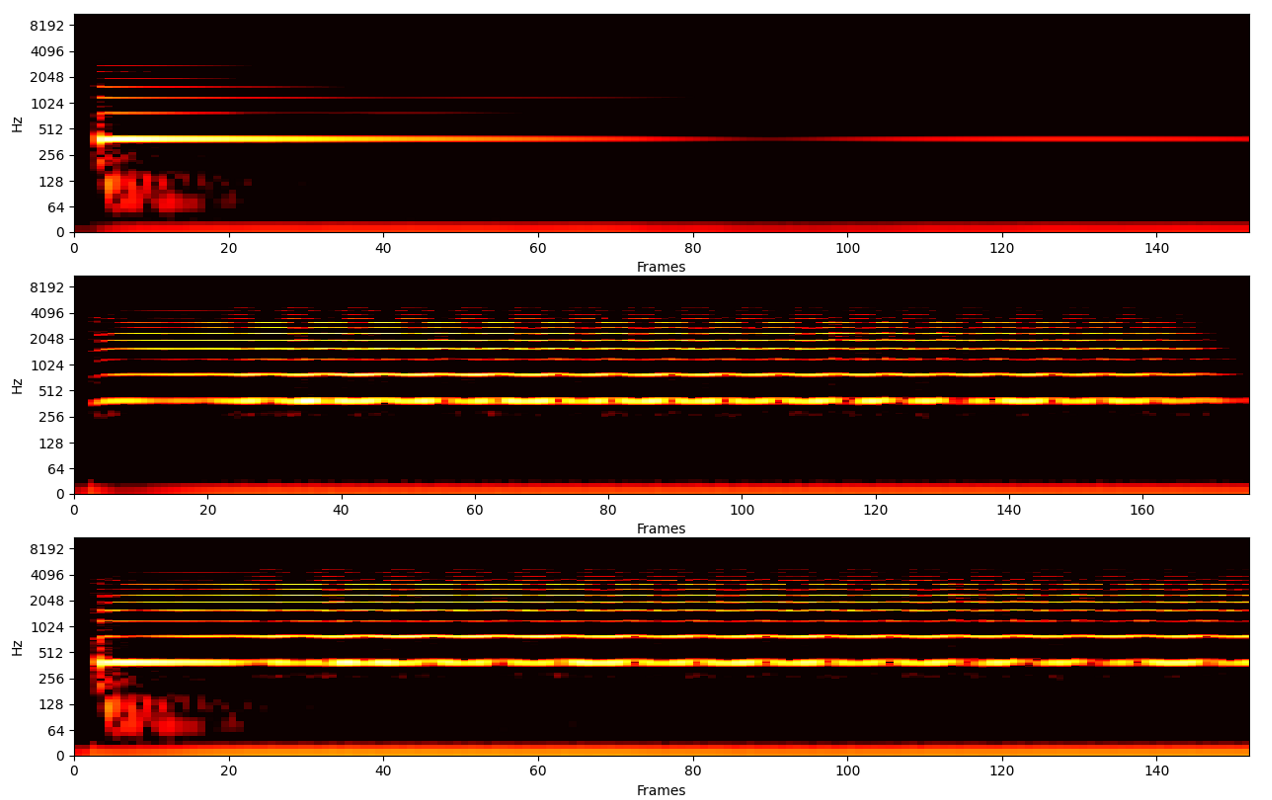
\includegraphics[width=\linewidth]{ch2/fig-G4-violin-piano.png}
    \caption{小提琴與鋼琴演奏G4音高三秒的特徵圖\ 上:小提琴,中:鋼琴,下:混合}
    \label{fig:fig-ch2-G4-violin-piano}
\end{figure}

雖然人耳可以輕易分辨出不同的音色,
但是當兩種聲音混合在一起時,要精準的將兩種樂器的聲音分開是一件困難的任務,
\cref{fig:fig-ch2-G4-violin-piano}的下方圖顯示了音訊混合後的特徵長相,
若要將兩種樂器的音源分離,我們必須精準地知道每個頻率原本的成分才有可能乾淨的分離。
音源分離的難度與樂器音色的複雜度、樂器種類的相似度而提高,因此至今音源分離的任務還是非常具有挑戰性。

另外在音樂追蹤方面,使用兩段相似的音訊特徵來追蹤是常見的方法,特徵越相近越容易有好的追蹤結果,
但若是屬於音色變化較大的樂器(例如小提琴),儘管是同一人演奏相同曲目兩次,特徵也不一定相同,
\cref{fig:fig-ch2-beethoven-violin-play-twice}顯示同一人使用相同速度、曲目演奏兩次的特徵圖,
雖然大致上看起來都相同,但細看的話在時間軸=100 frames時兩邊的特徵還是有些微的不同,
這些些微的不同之處都有可能會影響到追蹤結果。
\cref{fig:fig-ch2-bwv1006-two-different-violin}顯示不同人演奏同一首曲子的特徵圖,
可以看到這兩段音訊明顯在環境的收音上可能差很多,且在曲子的詮釋上也不完全相同,
使用這兩段音訊來追蹤,難度會比同一人演奏的版本要高很多,
因此使用不同音訊特徵來追蹤是具有一定的挑戰性。

\begin{figure}[H]
    \centering
    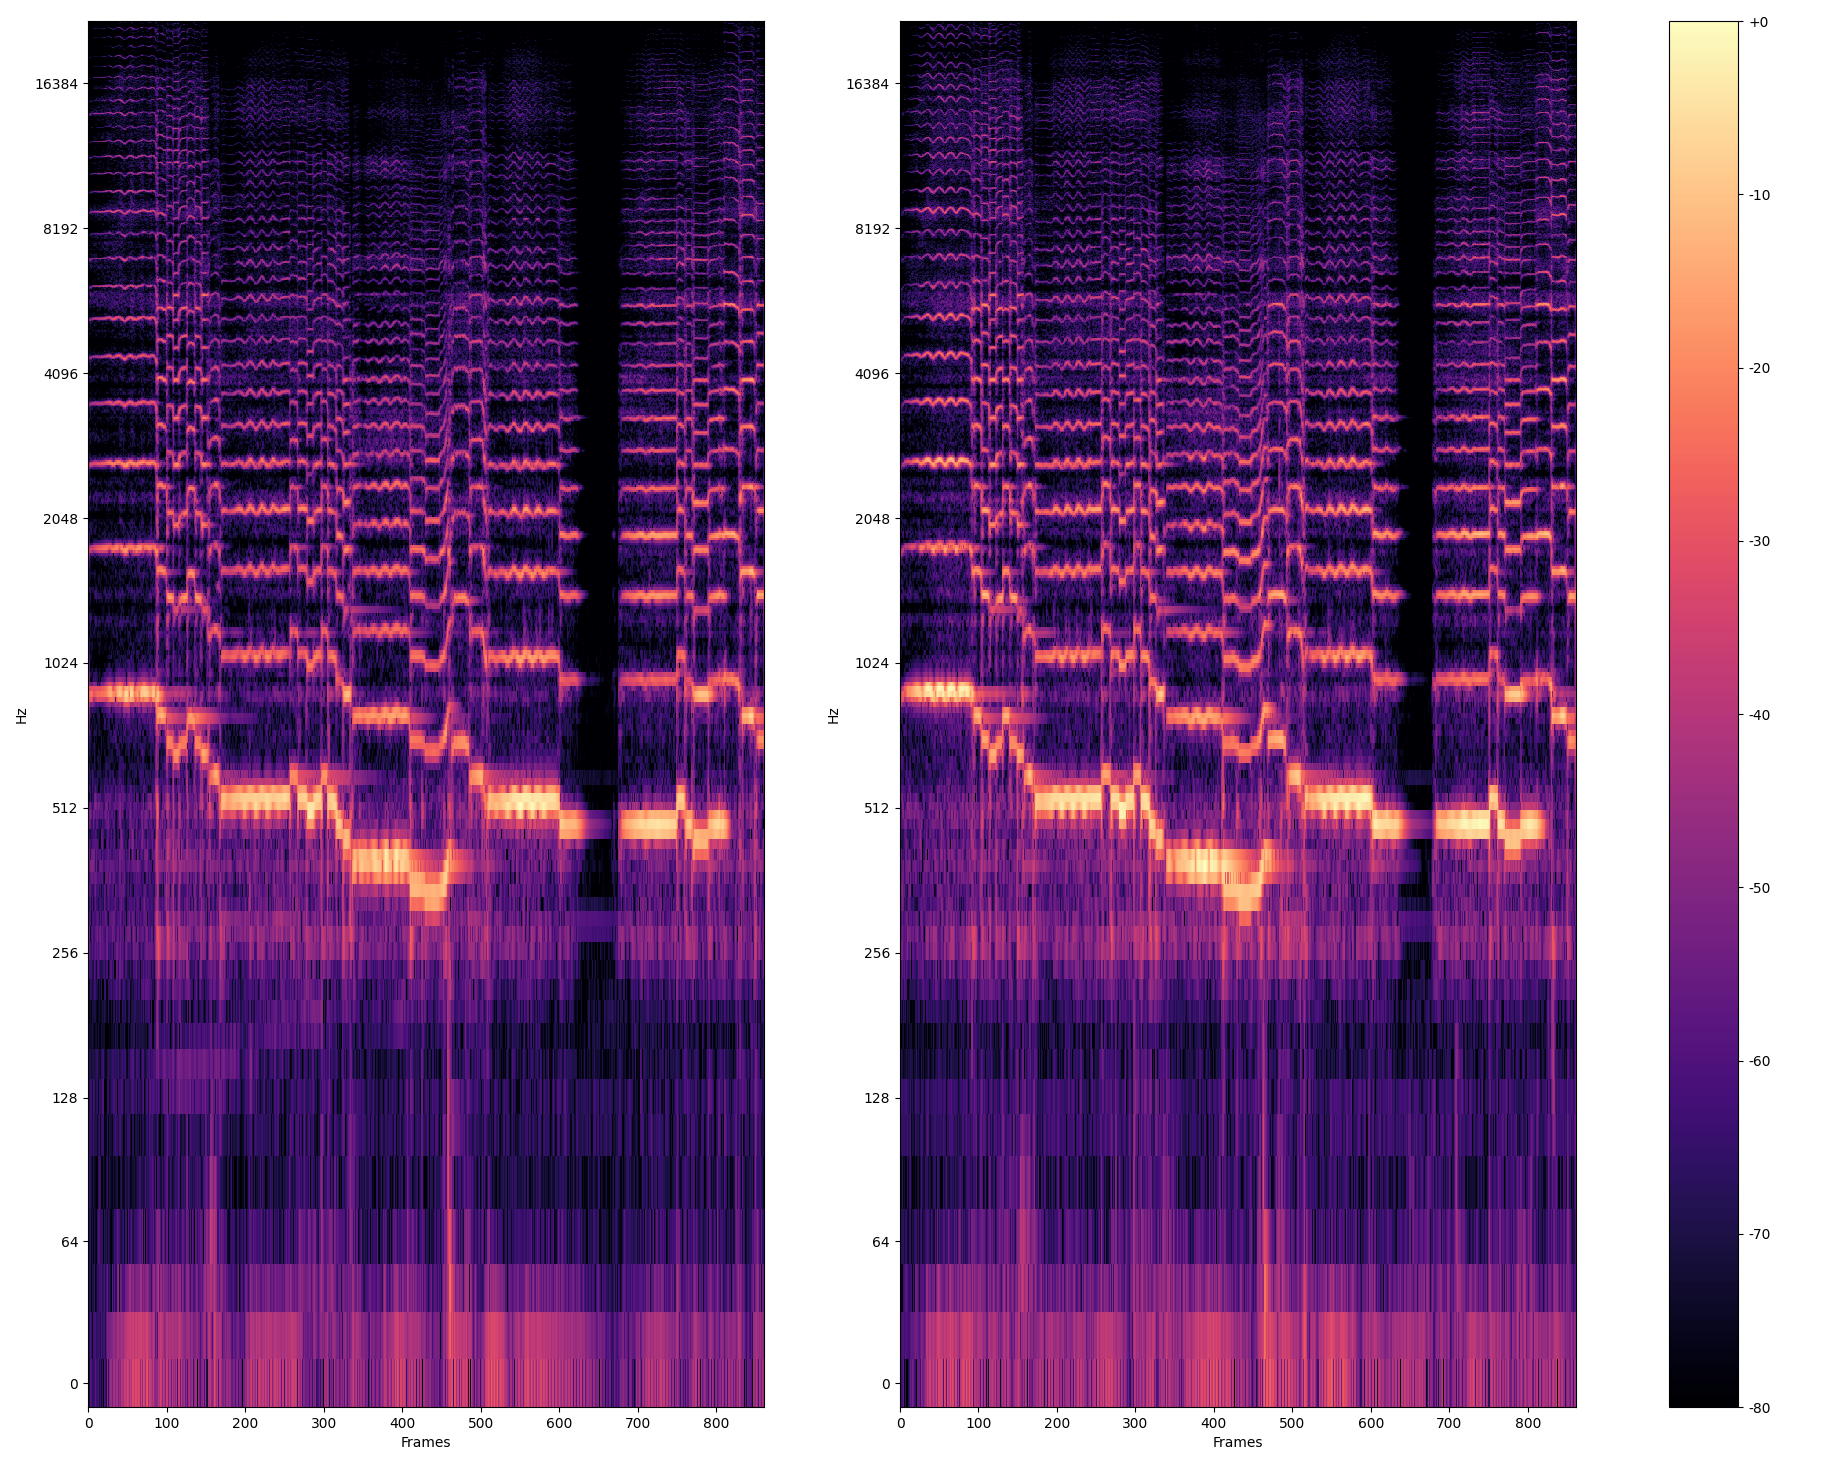
\includegraphics[width=1.0\linewidth, height=0.6\linewidth]{ch2/fig-beethoven-violin-play-twice.png}
    \caption{同一人演奏兩次 Beethoven Spring Sonata No.1 之特徵圖}
    \label{fig:fig-ch2-beethoven-violin-play-twice}
\end{figure}

\begin{figure}[H]
    \centering
    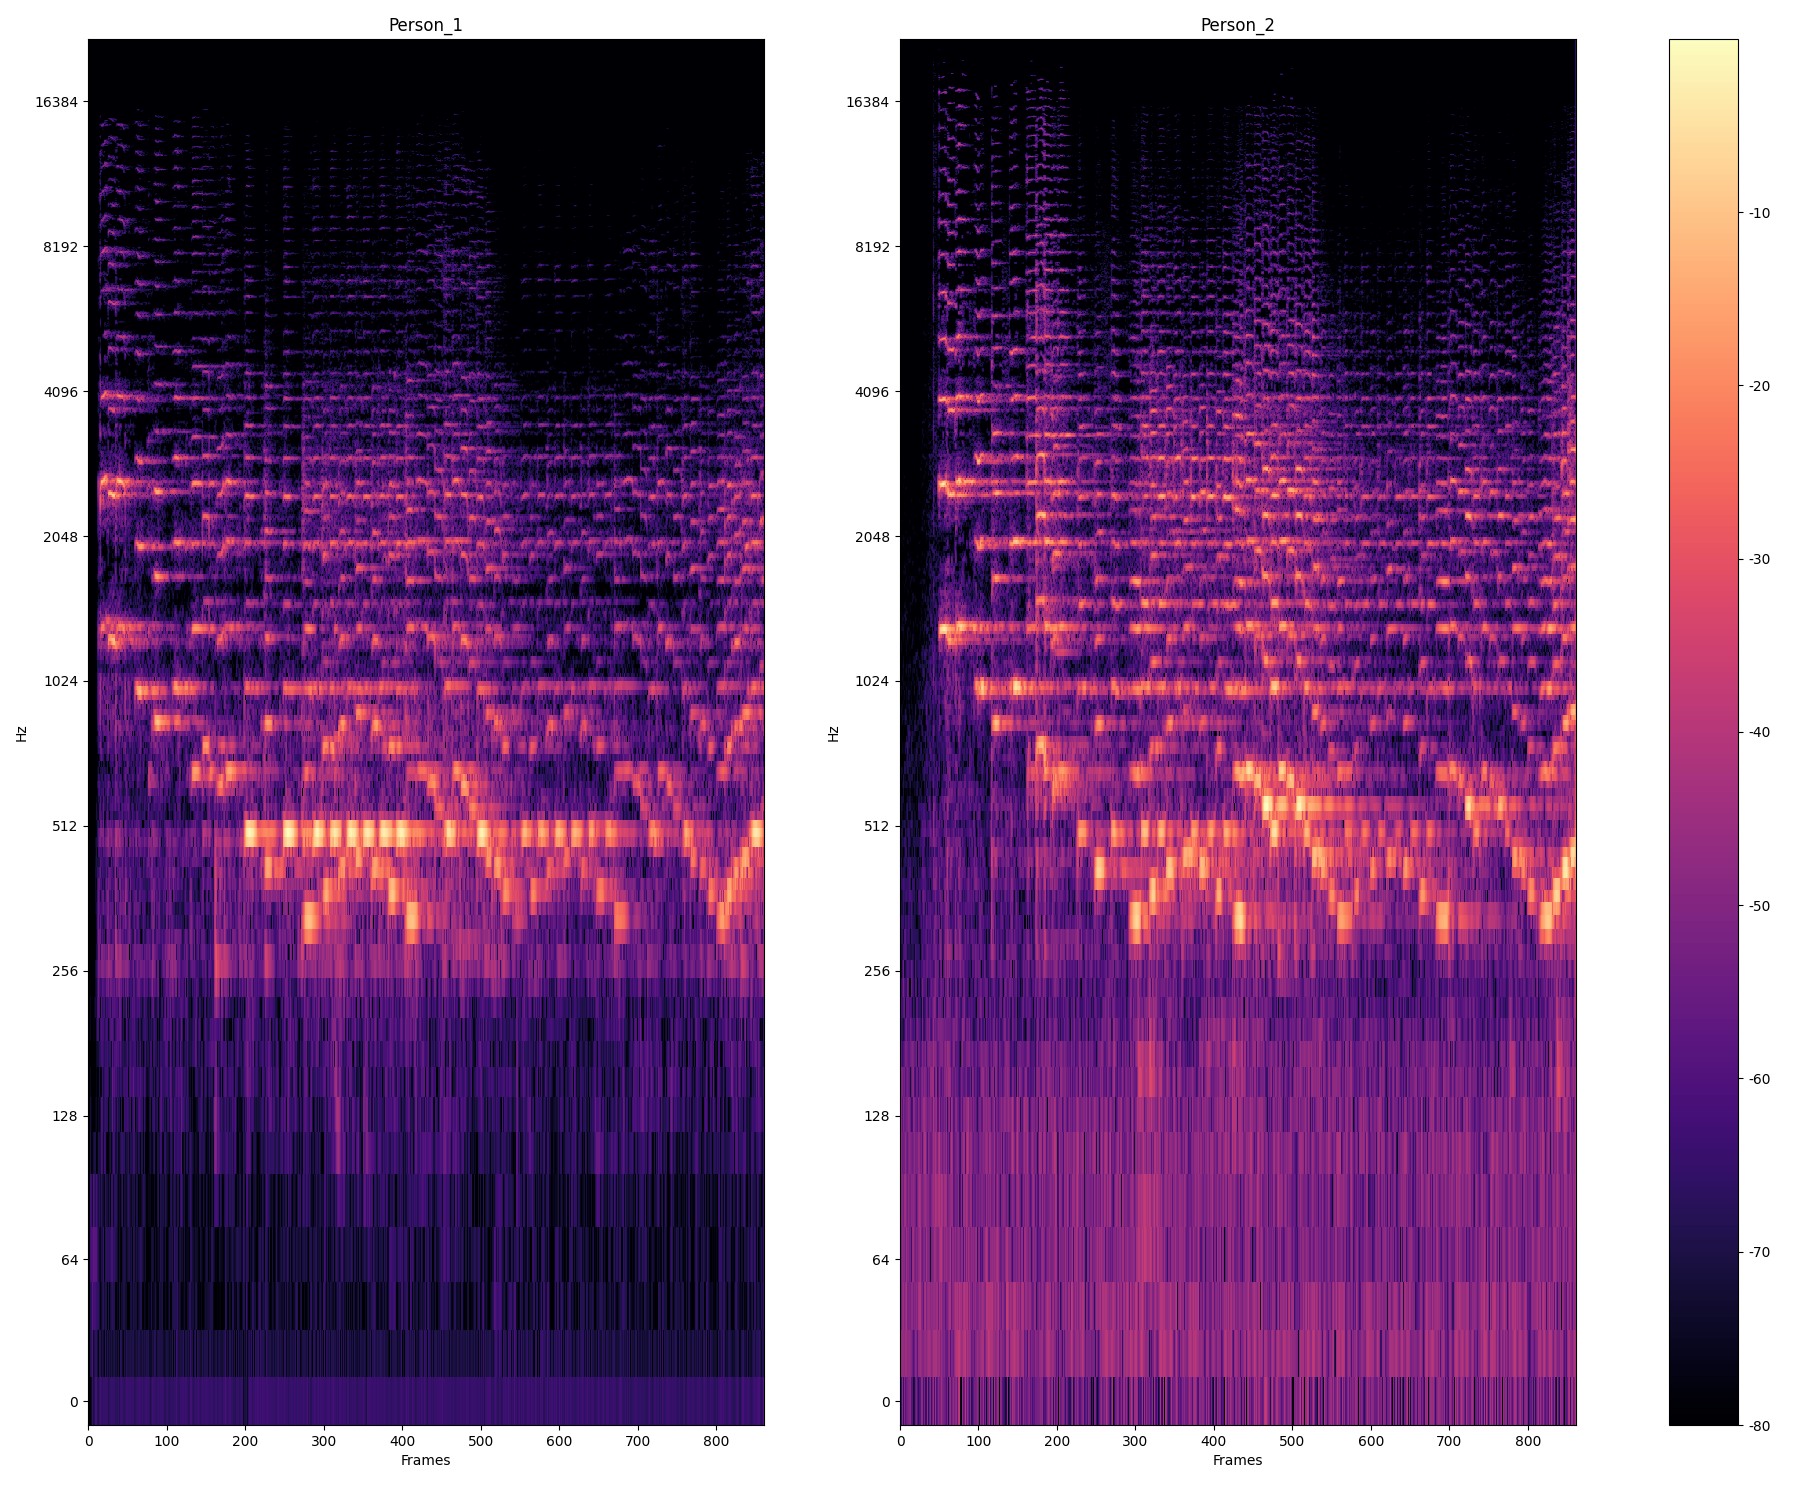
\includegraphics[width=1.0\linewidth, height=0.6\linewidth]{ch2/fig-bwv1006-two-different-violin.png}
    \caption{不同人演奏 Bach BWV1006 之特徵圖}
    \label{fig:fig-ch2-bwv1006-two-different-violin}
\end{figure}

\pagebreak

\section{文獻回顧}
\subsection{音源分離相關研究}
音源分離為MIR中的一個重要領域,日常生活中我們所聽到的音樂大多數是來自多個音源的混合音訊,
許多人可能希望調整混合音訊中的某種樂器的聲音平衡、改變聲音的空間位置,
甚至將混合音訊與每個存在於其中的音樂來源作為其他MIR任務的訓練資料,
因此,若是可以取得每個音樂來源的單獨音訊,上述所說的應用都能夠實現。

音源分離的目標最常見的為分離一首包含人聲、貝斯、鼓與其他(非前三者的所有音訊)的歌曲,
在大型音源分離比賽~\cite{Yuki_Mitsufuji2021MusicDemixing, Fabbro_Giorgio2023TheSoundDemixing}
中也是使用此標準進行。音源分離的方法可分為基於時間頻率表示方法與基於波形表示方法,
第一種通常會預測每個來源的功率頻譜,並結合輸入的混合音訊相位來合成每個音源的波形,
較傳統的方法有獨立成分分析(Independent Components Analysis, ICA)~\cite{comon1994independent},
此方法的目標是找到一個分離矩陣,使混合訊號透過分離矩陣計算出獨立的來源訊號;
非負矩陣分解(Non-negative Matrix Factorization, NMF)~\cite{lee2000algorithms}
為一種非監督式的機器學習技術,此方法是希望找到最好的兩個矩陣,使他們的乘積能接近原始的輸入。
然而這兩種方法對於複雜的混合音訊通常無法完全恢復單個音訊。
近年來隨著深度學習領域的蓬勃發展,越來越多研究使用全連接神經網路、LSTM、RNN等神經網路訓練頻譜圖。
2018年由Stöter等人所提出的Open-Unmix~\cite{FabianRobert_Stöter2019OpenUnmix}
模型在當時在公開資料集MUSDB~\cite{Rafii2017musdb18}上表現最佳,
此模型使用三層雙向LSTM對輸入預測一個遮罩,將混合音訊透過遮罩得到分離音源頻譜圖。
隨後在2022年由Luo Yi等人所提出的Band-Split RNN~\cite{Luo_Yi2022MusicSourceSeparation}
在MUSDB上取得最佳的SDR成績,此模型將輸入的頻譜圖分割為預先定義好頻帶寬度的子帶頻譜圖,
將子帶頻譜圖轉為相同維度的特徵後利用堆疊RNN交錯訓練,
最後經過MLP生成遮罩並與混合輸入結合產生分離音源頻譜圖,
至今仍是基於時間頻率訓練的開源模型中效果最佳的模型。
Open-Unmix與Band-Split RNN皆允許使用者自訂不同的分離目標,
使的這兩個模型擁有很高的靈活性。

第二種基於波形訓練的方法最早提出的模型為Wave-U-Net~\cite{stoller2018wave},
近年來較多人使用的Demucs~\cite{défossez2021music}就是基於Wave-U-Net的架構開發的,
Demucs為Encoder/Decoder架構,內部由卷積Encoder/Decoder與雙向LSTM組成,
Encoder與Decoder使用Skip U-net連接,將混合立體音訊作為輸入,輸出每個來源的估計波型。
2021年MDX競賽~\cite{Yuki_Mitsufuji2021MusicDemixing}
由Meta AI提出的冠軍模型Hybrid Demucs~\cite{defossez2021hybrid}更是將Demucs擴展為多域分析的架構,
模型變為由波型、頻譜和共享層組成。2022年Meta AI結合先前的結果提出了
Hybrid Transformers~\cite{rouard2023hybrid},將Encoder/Decoder內部兩層替換為跨域Transformer,
使的模型可以接受異質資料,變成更靈活的架構,並在MUSDB的SDR表現上為9.20dB,
為目前所有開源模型中最佳的模型。

在古典樂器錄音的音源分離研究中,比起音高樂器(例如:吉他)與非音高樂器(例如:鼓)的音源分離情況更有挑戰性,
且公開資料集的蒐集難度高,訓練資料驅動模型的難度也更大。
因此針對這些資料通常會使用資料增強的方法來增加訓練資料,
由Miron等人提出的CNN-based低延遲單聲道源分離模型~\cite{miron2017generating},
透過改變速度、音色、動態時間局部變化來增加新的訓練資料,使模型在實際情況下更能應對演奏時的狀況。
由Chiu Ching Yu等人提出針對資料規模小的資料集的資料增強方法~\cite{Chiu_ChingYu2020MixingSpecific},
使用Open-Unmix模型訓練並在針對小提琴與鋼琴的混合音源分離的任務上,
比當時可用的最佳模型Spleeter~\cite{hennequin2020spleeter}的效果要好。

本研究將使用靈活性高且較輕量的Band-Split RNN~\cite{Luo_Yi2022MusicSourceSeparation}模型,
針對小提琴與鋼琴的混合音源資料做訓練,旨在促進古典樂器錄音的音源分離研究進展。

% 引用音源分離的相關論文並進一步討論

\subsection{音樂追蹤相關研究}
音樂追蹤在MIR領域中是一項重要的應用,與節拍追蹤~\cite{heydari2021don, goto2021musical, di2021downbeat}、
樂譜追蹤~\cite{henkel2019score}、自動伴奏~\cite{zhang2023design}等相關技術有密切的關係,
本節專注探討以音訊特徵為主的即時音樂追蹤的方法與應用的相關研究。
音樂追蹤的方法包含隱藏馬爾科夫模型(Hidden Markov Model, HMM)~\cite{cano1999score},
HMM透過樂譜中的狀態迭帶訓練目前追蹤的位置,但也因為需要大量標註過的資料,在即時表現方面較為遜色;
動態時間規整(Dynamic Time Warping, DTW)~\cite{Arzt2012Adaptive, Raffel2016Optimizing}為最多人使用的方法之一,
DTW透過計算兩段相似序列的成本矩陣,回推最佳對齊點,由於音樂的連續性使的DTW計算結果準確率高,
但也因為計算時間複雜度高而無法應用在即時音樂追蹤。
因此許多人對DTW演算法改良了更快速的版本,例如平行化動態時間規整(Parallel Dynamic Time Warping, PDTW)~\cite{Wei2018Online},
PDTW將兩個時間序列分割成多段的序列,每段序列各自計算DTW,計算完畢後再將每段序列連接回整段,
加速DTW的運算時間;線上動態時間規整(Online Dynamic Time Warping, ODTW)~\cite{dixon2005ODTW, Arzt2010Towards, Lin2020AHumanComputerDuetSystem}
將原本DTW向後對齊的模式改為增量對齊,ODTW不需要事先取得兩段序列的資訊,
而是根據每個時間點計算出的路徑決定下一步的方向,因此ODTW在即時音訊的處理的情況會比前面提到的方法還要快速,
更能達到即時音樂追蹤的效果。

音樂追蹤使用的音訊通常越相像越好,例如使用同一人事先演奏的音訊來追蹤同一人的現場演奏,
但通常使用者並不會特意去錄製事先演奏的音訊,尤其是在沒有合奏者的情況下,
因此本研究致力於研究不同特徵的即時音樂追蹤系統。
本研究將基於~\cite{Lin2020AHumanComputerDuetSystem}所提出的架構進行重新實現並改良部分方法,
希望能藉此達到我們所期望的效果並促進即時音樂追蹤研究進展。

% DTW、DTW的各種變形、ODTW、RL、
% 引用音樂追蹤的相關論文並進一步討論

\pagebreak

\end{document}    % 背景知識及文獻回顧
        \documentclass[class=NCU_thesis, crop=false]{standalone}
\begin{document}

\chapter{研究方法}

\section{系統架構} \label{ch3-st-system-structure}
\fig[1][fig:fig-ch3-system-structure-overview][!hbt]{ch3/fig-system-structure-overview.png}
[系統架構圖][系統架構圖]

\cref{fig:fig-ch3-system-structure-overview} (A)
為本系統的整體架構,此系統可分為離線處理與線上處理兩個階段,
離線處理階段會將混合音源分離成參考音訊與伴奏音訊作為線上處理階段的資料,
線上處理階段接收演奏者的即時串流音訊,並結合參考音訊來計算目前演奏者的樂曲位置,
並根據樂曲位置輸出對應的伴奏音訊。
請注意本研究將小提琴與鋼琴之混合音訊作為主要資料,
並專注在當演奏者樂器為小提琴或鋼琴的狀況下來使用本系統。

\cref{fig:fig-ch3-system-structure-overview} (B)
為音源分離模組的細部架構,
採用深度學習模型將混合音訊中的目標音源分離出來。
此模組包含了小提琴(參考音訊)音源分離模型與鋼琴(伴奏音訊)音源分離模型,
另外在訓練階段,本研究設計了一種簡單的頻帶切割估計方法提升模型的分離效果。
關於模型架構、頻帶切割估計方法會在\ref{ch3-st-mss-module}節做討論。

\cref{fig:fig-ch3-system-structure-overview} (C)
為音樂追蹤模組的細部架構,
此模組使用Python 3.9開發,
我們使用multiprocessing package~\cite{python2024multiprocessing}實現平行化處理,
串流音訊使用pyaudio package~\cite{python2024pyaudio}接收處理,
達到即時伴奏的效果。
此模組包含四個元件,
分別為Data Manager、Music Detector、Rough Position Estimator與Decision Maker。
Data Manager管理所有音訊的資料與特徵、
Music Detector即時偵測音樂是否開始、
Rough Position Estimator粗略估計可能的伴奏時間位置,提供Decision Maker更多選擇、
Decision Maker即時計算目前輸出位置並決定最後的輸出位置,
關於元件詳細的設計與改動會在\ref{ch3-st-music-tracking-module}節做討論。

\pagebreak

\section{音源分離模組} \label{ch3-st-mss-module}

\subsection{Band-Split RNN} \label{ch3-subst-band-split-RNN}
Band-Split RNN (BSRNN)~\cite{Luo_Yi2022MusicSourceSeparation}
由Luo Yi等人於2022年提出,是一種專門為高取樣率訊號所設計的時頻域音源分離模型。
BSRNN將輸入的頻譜圖$X\in \mathbb{C} ^{F\times T}$
根據自定義的頻帶切割點$G = (G_1, G_2, \dots G_i), \sum_{i = 1}^{K} G_i = F $
拆分成一個個的子帶頻譜圖$B = (B_1, B_2, \dots B_K), B_K \in \mathbb{C}^{G_K\times T}$,
每個不同大小的子帶頻譜圖經過處理後變為一系列具有相同維度的特徵$Z\in \mathbb{R}^{N\times K\times T}$,
接著利用RNN層將頻帶與序列的資訊交錯建模得到輸出$Q\in \mathbb{R}^{N\times K\times T}$,
最後每個子帶特徵由多層感知器 (MLP)產生對應的複值時頻遮罩$M\in \mathbb{C}^{F\times T}$,
並將遮罩用於輸入的混合頻譜圖來產生估計的目標源頻譜圖$S\in \mathbb{C}^{F\times T}$。
整體架構如\cref{fig:fig-ch3-BSRNN-model-structure}所示。

\fig[1][fig:fig-ch3-BSRNN-model-structure][!hbt]{ch3/fig-BSRNN-model-structure.png}
[BSRNN架構圖,擷取自~\cite{Luo_Yi2022MusicSourceSeparation}][BSRNN架構圖,擷取自~\cite{Luo_Yi2022MusicSourceSeparation}]

其中在\cref{fig:fig-ch3-BSRNN-model-structure} (B) 
的頻帶切割模組是BSRNN模型中最重要的模組,
此模組可根據目標音源的聲音特性來設計不同的頻帶切割範圍,
例如當目標音源的聲音特性都集中在較低頻的地方時,我們可以將低頻切割得更細,
高頻切割的寬一點,使模型在訓練時可以看到更重要的頻域特徵。

\subsection{估計不同樂器的頻帶切割點} \label{ch3-subst-estimate-band-split-point}
為了使頻帶切割模組(\cref{fig:fig-ch3-BSRNN-model-structure} (B))發揮更好的效果,
我們使用簡單的頻帶切割估計方法來估計小提琴與鋼琴的頻帶切割點,
此方法不需要依賴先驗知識或專家知識的幫助,而是透過同一種樂器的音訊資料來估計頻帶切割點。
首先我們對每種樂器選取約15分鐘的的音訊資料,這些資料並不會加入模型的訓練。
接著定義每種樂器的切割比例閥值$r$、
最小頻率切割值$f_{min}=100$Hz、取樣率$sr = 44100$Hz
與初始頻帶陣列$F_{band} \in \frac{sr}{2} $,
本研究之兩種樂器的切割比例閥值為$r_{violin}=0.013$, $r_{piano}=0.0035$,
此數值是根據計算出來的切割頻帶數量去做調整。

對於每筆資料,使用快速傅立葉轉換計算頻率域的每個樣本得到的振幅與對應到的頻率,
由於FFT的對稱性,我們只需要迭帶一半的樣本數,並將振幅值累加到對應的$F_{band}$。
累加振幅值越高代表此頻率的重要程度越高,如\cref{fig:fig-ch3-bandwidth-estimate}所示。
\begin{figure}[H]
    \centering
    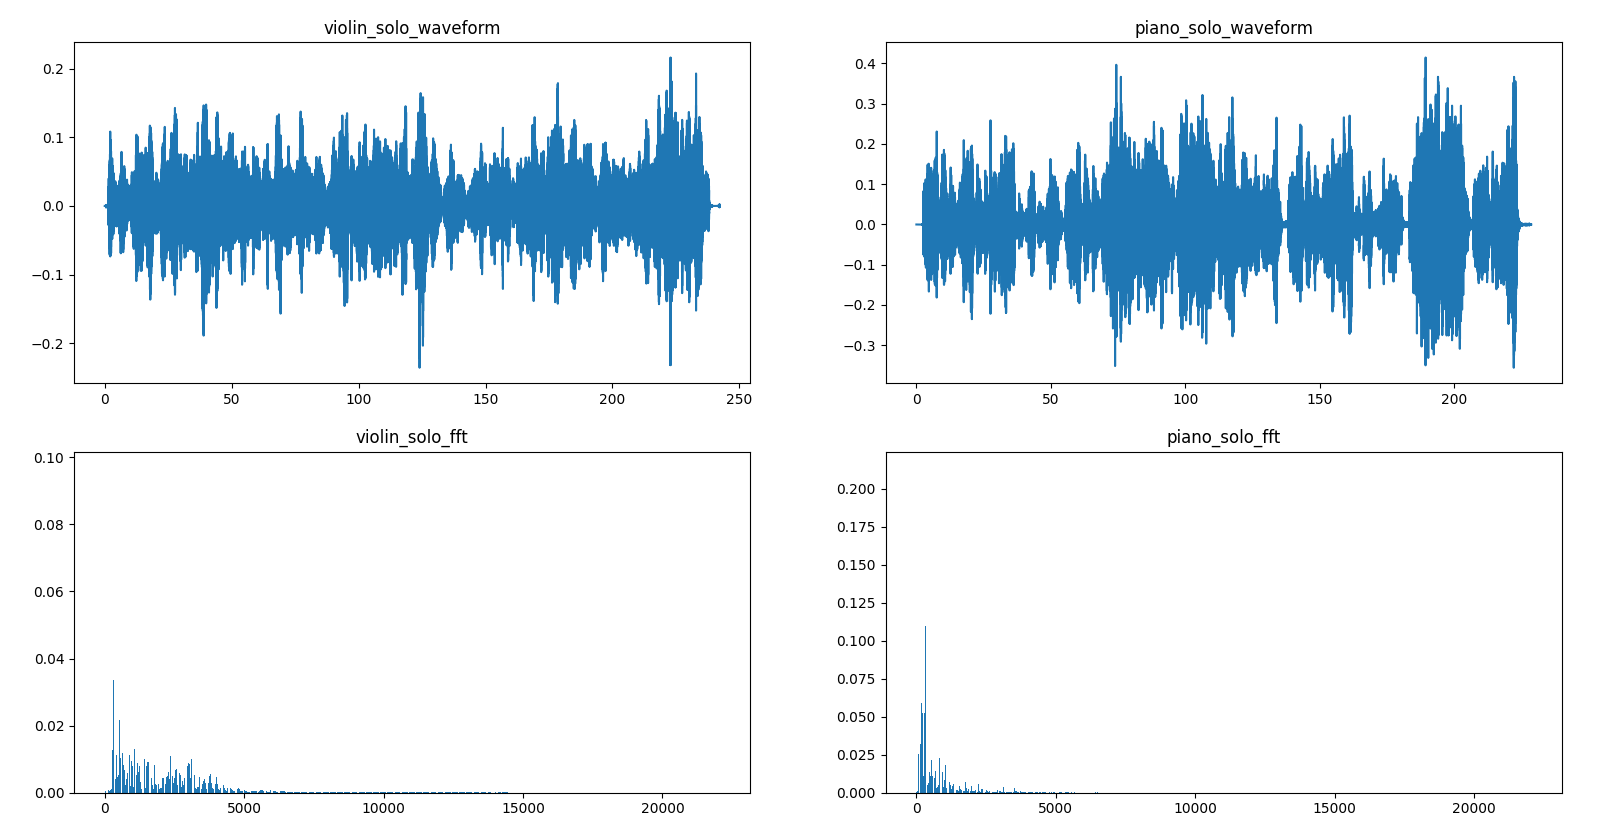
\includegraphics[width=\linewidth]{ch3/fig-bandwidth-estimate.png}
    \caption{兩種資料的波形圖(上)與經過FFT轉換後的$F_{band}$圖(下)}
    \label{fig:fig-ch3-bandwidth-estimate}
\end{figure}

最後我們對$F_{band}$的範圍迭帶計算每個區間的累積振幅值占總和值
的比例$f_{range}/\sum F_{band}$,若超過切割比例閥值$r$,則在此頻率點增加一個切割點。
依照上述的切割比例我們得到兩種樂器的頻帶切割點為 \\
\\
Violin = [400,500,600,700,800,900,1000,1100,1200,1300,1500,1600,1700,1800,\\
1900,2000,2100,2300,2400,2500,2600,2700,2800,2900,3000,3200,3400,3600,3800,\\
4000,4200,4500,4800,5300,5800,6500,7400,8600,10400,13000,18000]\\
\\
Piano = [100,200,300,400,500,600,700,800,900,1000,1100,1200,1300,1400,1500,\\
1600,1700,1800,1900,2000,2100,2200,2300,2400,2500,2600,2700,2800,2900,3000,\\
3200,3400,3600,3900,4100,4400,4800,5300,5900,6900,8700,17300]\\
\\
在訓練Band-Split RNN模型時我們將會套用上面兩個頻帶切割範圍做訓練。

\pagebreak

\section{音樂追蹤模組} \label{ch3-st-music-tracking-module}
此模組是參考~\cite{Lin2020AHumanComputerDuetSystem}的real-time music tracker來重新實現,
本節將分成兩個部分說明,
\ref{ch3-subst-DTW}節至\ref{ch3-subst-GBA}節
會介紹實現音樂追蹤模組所使用到的演算法並詳細說明改進的部分,
\ref{ch3-subst-data-manager}節至\ref{ch3-subst-decision-maker}
會介紹每個元件的設計與改動。

\subsection{動態時間規整演算法} \label{ch3-subst-DTW}
動態時間規整演算法(DTW)~\cite{Sakoe1978Dynamic},
是一種用來計算兩個時間序列資料之間相似度的方法。
給定兩個時間序列
$X = (x_1, x_2, \dots x_N), N \in \mathbb{N}$和
$Y = (y_1, y_2, \dots y_M), M \in \mathbb{M}$,
其中N和M為兩個時間序列的長度,
$x_N$和$y_M$是任兩個具有時間順序且形狀相似的資料,例如音樂、語音等等,
如\cref{fig:fig-ch3-dtw-example}所示。
\begin{figure}[!hbt]
    \centering
    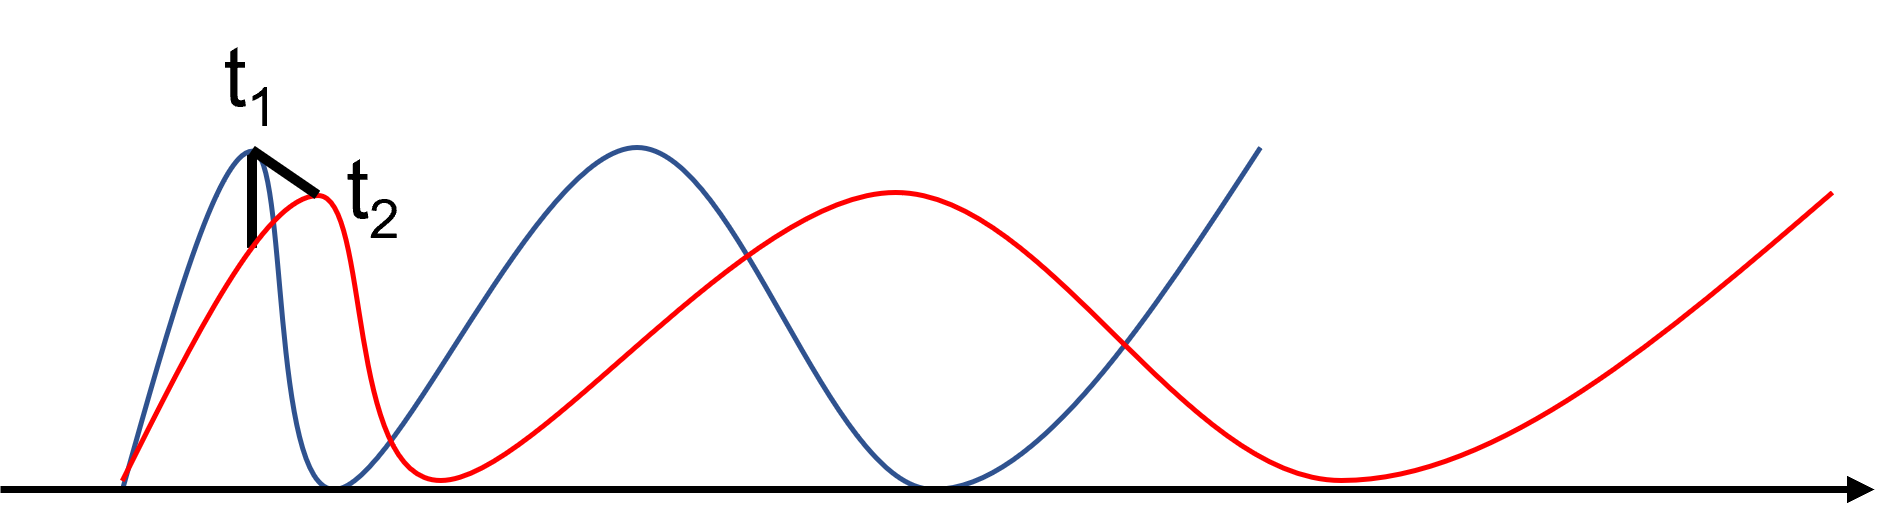
\includegraphics[width=\linewidth]{ch3/fig-dtw-example.png}
    \caption{兩個相似的時間序列:藍色: $X$\ 紅色: $Y$}
    \label{fig:fig-ch3-dtw-example}
\end{figure}

可以看到計算$X[t_1]$與$Y[t_1]$的距離,並不會是相似的資料點,
但若計算$X[t_1]$與$Y[t_2]$的距離,就會被認為是兩個相近的資料點,
因此當兩段相似的資料但在時間軸上並不是對齊的,就適合用DTW演算法動態對齊時間。
考慮到時間序列的長度不一定相等的情況,例如不同人演奏同一個音符可能會有不同的速度差異,
因此DTW通常採用動態規劃的方法來計算相似度。

首先使用歐基里德距離\cref{eq:compute-dtw-cost-function}
計算X與Y所有時間點的距離,
\begin{equation}
    \label{eq:compute-dtw-cost-function}
    d(i, j) = \sqrt{\left\lvert x_i-y_j\right\rvert^{2}}
\end{equation}

並根據\cref{eq:compute-dtw-cost-matrix-function}
使用動態規劃方式建立距離矩陣$D \in \mathbb{R}^{N \times M}$。
\begin{align}
    \label{eq:compute-dtw-cost-matrix-function}
    \left\{
        \begin{array}{l}
            D(0, 0) = d(x_1, y_1)\\
            D(i, 0) = D(i-1, 0)+d(x_i, y_1)\\
            D(0, j) = D(0, j-1)+d(x_1, y_j)\\
            D(i, j) = d(x_i, y_j) + \min \left\{
                \begin{array}{l}
                    D(i, j-1) \\
                    D(i-1, j) \\
                    D(i-1, j-1)
                \end{array}\right\}
        \end{array}
    \right.
\end{align}

在計算最短路徑時,必須遵守三個限制:
\begin{enumerate}
    \item 邊界限制:路徑的開頭與結束必須為$(x_1,y_1)$與$(x_N,y_M)$
    \item 連續性:若路徑的上一個對齊點為$(i, j)$, 
    下一個對齊點只能是$(i+1, j+1), (i+1, j), (i, j+1)$
    \item 單調性:若路徑的上一個對齊點為$(i, j)$,
    下一個對齊點必須為$(i_{next}, j_{next}) \in (i_{next} \geq i, j_{next} \geq j)$
\end{enumerate}
這是為了使回溯的路徑為連續無倒退且整段序列都被包含在輸出裡,確保對齊的一致性。

最後從$D(N, M)$往前回溯至$D(1, 1)$尋找一條最小的累積距離成本路徑,
計算公式如\cref{eq:dtw-backtracking-function}所示,
選擇回溯點時會確認行、列與對角三個方向的距離成本值,並選擇成本最小的點作為回溯點,
\begin{equation} 
    \label{eq:dtw-backtracking-function}
    \begin{cases}
        \text{$(i_{next}, j_{next}) = argmin_{(i-1,j-1),(i-1,j)(i,j-1)}D(i_{next}, j_{next})$} \\
        \text{Stop},\qquad \text{if $(i, j) = (1, 1)$} 
    \end{cases}
\end{equation}

當回溯點走到起始點$(1, 1)$時,將所有回溯點連起來就得到最後對齊路徑$W$,
如示意\cref{fig:fig-ch3-dtw-path-example}所示,右上角為路徑的結束位置$D(N, M)$,
左下角為路徑的開始位置$D(1, 1)$,綠色路徑即為$W$。
\begin{figure}[!hbt]
    \centering
    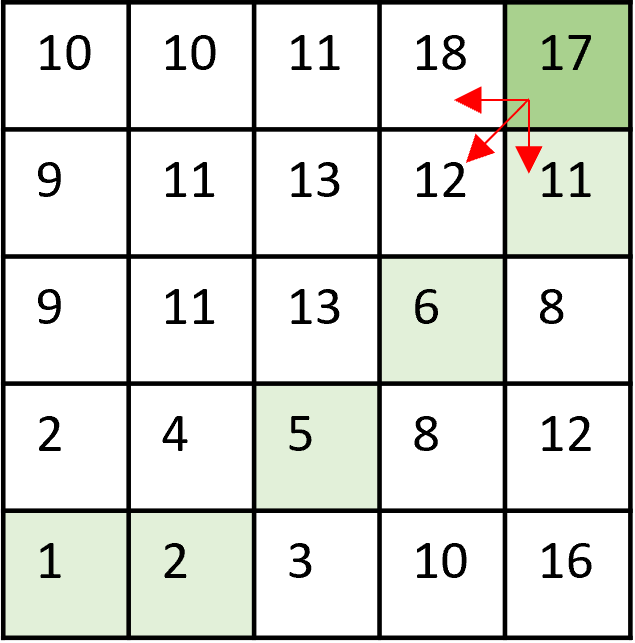
\includegraphics[width=0.4\linewidth, height=0.4\linewidth]{ch3/fig-dtw-path-example.png}
    \caption{DTW 累積距離矩陣回朔路徑示意圖}
    \label{fig:fig-ch3-dtw-path-example}
\end{figure}

本研究所使用的DTW演算法來自python librosa package~\cite{McFee2024librosa}
中的librosa.sequence.dtw函式。

\subsection{線上動態時間規整演算法} \label{ch3-subst-ODTW}
由於DTW演算法在時間複雜度上為$O(NM)$,屬於複雜度高的演算法,
因此當某個序列的時間較長或是不確定序列的時間長度(例如即時串流音訊)時,
DTW演算法在計算就會花費許多時間。

線上動態時間規整演算法(ODTW)~\cite{dixon2005ODTW}由Dixon等人提出,
是基於DTW演算法所做的改良,首先ODTW在計算對齊路徑時並不是回溯計算而是向前增量計算,
並且將計算距離成本的範圍縮小至預先定義的範圍$c$,
因此使ODTW在時間與空間複雜度的表現都是線性$O(N)$,
且因為不需事先知道整個序列的資料,因此適合處理長序列音訊或即時串流音訊。

本研究實現ODTW演算法的步驟如下,
給定兩個時間序列
$X = (x_1, x_2, \dots x_N), N \in \mathbb{N}$和
$Y = (y_1, y_2, \dots y_M), M \in \mathbb{M}$,
其中$X$為現場音訊,因此$N$會隨著串流時間長度而增加,直到串流結束,
$Y$為事先給定的參考音訊,用於對齊現場音訊。
我們想透過距離成本矩陣$D_{total}$找到$X$和$Y$的對齊路徑$W = (W_1, W_2, \dots W_k)$,
其中每個$W_k$為有順序的$(i_k,j_k)$且
$(i,j) \in W$代表兩段序列在$x_i$與$y_j$點上對齊。

距離成本矩陣$D_{total}$透過\ref{ch3-subst-DTW}節所提到的\cref{eq:compute-dtw-cost-function}與
\cref{eq:compute-dtw-cost-matrix-function}計算,另外我們使用$D_{cell}$紀錄單格的距離成本$d$。
我們定義搜尋範圍$c=450$來限制$D_{total}$與$D_{cell}$的大小,
當有新的$i$加入時,我們計算$d(i, j-c), d(i, j-c+1) \dots d(i, j+c)$個點,
此時$j$為目前演算法計算到的參考音訊時間點,而對於$j$點,
則是計算$d(i-c, j), d(i-c+1, j) \dots d(i, j)$,
由於我們無法得知未來的現場音訊,所以只能計算到目前最新的時間點$i$。
上述的計算方式與傳統的ODTW演算法有些微的不同,
在~\cite{dixon2005ODTW}中,每次迭帶時在(i, j)方向計算的格數皆為$c$個,
我們將每次迭帶在j方向計算的cell個數改為$2c-1$,
如範例\cref{fig:fig-ch3-odtw-search-range-compute-comparision}所示。
\begin{figure}[!hbt]
    \centering
    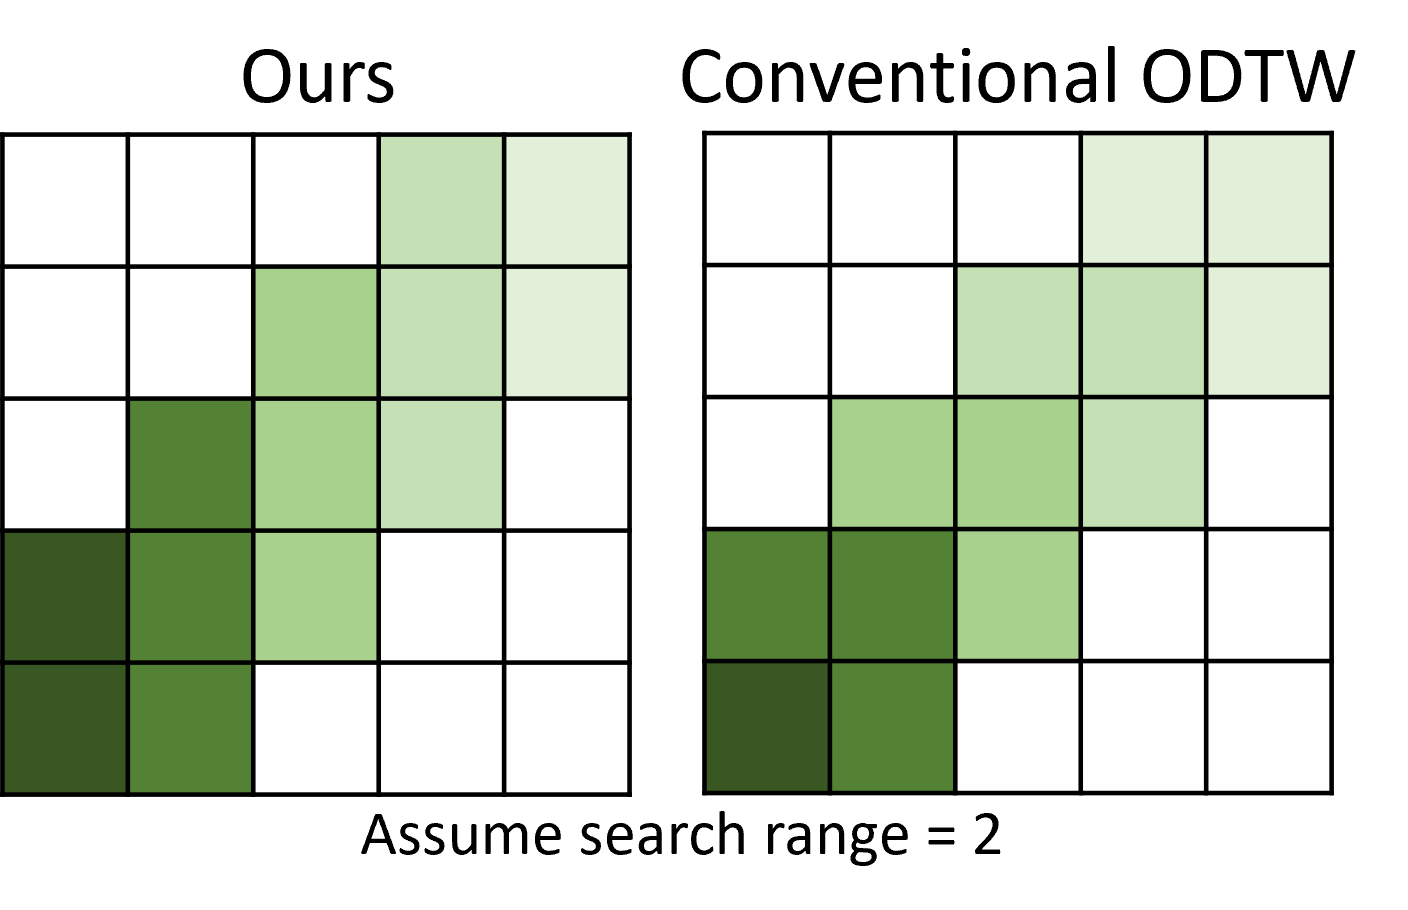
\includegraphics[width=0.8\linewidth]{ch3/fig-odtw-search-range-compute-comparision.png}
    \caption{每個迭帶所計算到的距離成本矩陣格數位置比較}
    \label{fig:fig-ch3-odtw-search-range-compute-comparision}
\end{figure}

會做這樣的更動是因為我們的$i$為現場串流音訊的時間點,
而串流音訊並不會出現相同的時間點(輸出永遠為嚴格單調遞增),
且我們無法得知目前現場音訊的快慢,
因此為了能讓最後輸出對齊位置時有更多的選擇,
我們除了向前計算,也向後計算參考音訊的距離成本。

在計算完目前$(i, j)$的距離成本矩陣後,
我們需要決定下一步的$(i_{next}, j_{next})$走向以增加新的距離成本到兩個矩陣中。
由於我們將$i$設定為嚴格單調遞增,因此在決定增量對齊的方向時,
只會有$(i+1, j+1)$與$(i+1, j)$兩種方向。
除非在同一個方向增加超過事先設置的參數$ODTW_{Max\_Run} = 3$,
否則我們每次都會計算$(i+1, j+1)$方向。
另外當目前的$i < c$時,為了使搜索範圍內的格數有計算到完整的距離成本,
即使$output_j \neq j$,在下一個迭帶我們還是計算點$(i+1, j+1)$,
直到$i >= c$時才會將$j$設為$output_j$。

在每次計算完最新的$D_{total}$與$D_{cell}$後,
我們使用這兩個成本矩陣計算時間點$i$的對齊位置$output_j$,
首先我們設定兩個參數$L_{upper} = (j+ODTW_{Max\_Run}\times 10)$,
$L_{lower} = (j-1)$,分別代表尋找$output_j$的上下限,
迭帶所有介於$L_{upper}$與$L_{lower}$的點$curr_{j}$,
找到一組點$(i, curr_{j})$的$D_{total}(i, curr_{j})+D_{cell}(i, curr_{j})$值為最小值,
$(i, curr_{j})$即為ODTW的輸出對齊點。

\subsection{貪心向後對齊方法} \label{ch3-subst-GBA}
由於ODTW在對齊時為增量對齊,並不像DTW一樣在計算完兩段音訊的成本矩陣後才回溯最佳對齊路徑,
因此通常ODTW的輸出結果會比DTW的輸出結果來的更不穩定。
為了改善上述問題,我們參考~\cite{Arzt2010Towards}中的Greedy Local Search演算法
來設計Greedy Backward Alignment (GBA)方法,
此方法配合多執行續的執行可以快速的計算目前位置的向後對齊成本。

給定一個預計輸出位置$(i, j)$作為向後對齊的結尾點,
此位置代表在現場音訊為$i$時,參考音訊估計的對齊位置為$j$,
我們設定一個向後對齊距離參數$GBA_{t}$,
根據現在$i$的時間點與先前輸出位置紀錄$W_{output}$,
我們可以推算出向後對齊的開頭點$(i_{prev}, j_{prev}) = W_{output}[i-GBA_{t}]$。

接著根據距離成本矩陣$D$,我們可以透過\ref{ch3-subst-DTW}節的\cref{eq:dtw-backtracking-function}
計算$(i_{prev}, j_{prev})$到$(i, j)$的對齊成本$W_{cost}$,
在回溯的過程中,因為$(i_{prev}, j_{prev})$與$(i, j)$並不是真正的起始與結束點,
我們設定了最大步數$GBA_{Max\_Run}=3$來限制回溯路徑的走向,
若過程中在行或列的方向走超過$GBA_{Max\_Run}$,
下一步只計算其他兩種方向的對齊成本決定走向。
另外在計算累積距離成本時,我們紀錄回溯路徑的總步數$step_{total}$,
並針對三種走向設計不同大小的值,當走向為對角時,$step_{total}$增加2步,
當走向為行或列時,$step_{total}$增加1步。
這是為了正規化總累積成本,
使每個預計輸出位置在比較累積距離成本時能公平的比較,
最後對齊成本計算公式如\cref{{eq:compute-backtracking-cost-function}}所示。
\begin{equation}
    \label{eq:compute-backtracking-cost-function}
    W_{cost} = \frac{\sum_{w = (i_{prev}, j_{prev})}^{(i, j)}D(w)}{step_{total}} 
\end{equation}

% 解釋為何需要、
% 從候選位置中挑選最好的path、
% 說明參數的設定

% \subsection{即時追蹤系統設計}
% 在音樂追蹤模組中,若無法即時的處理串流音訊導致系統阻塞,就無法達到即時伴奏的效果。
% 因此

\subsection{Data Manager Block} \label{ch3-subst-data-manager}
在線上處理階段啟動前與啟動後,
我們對非串流音訊(參考音訊、伴奏音訊)與串流音訊(現場音訊)
擷取兩種特徵作為其他元件的輸入資料,
分別為高解析度特徵與低解析度特徵,高解析度特徵為梅爾頻譜特徵,
低解析度特徵為高解析度特徵對時間軸卷積後的重新採樣。
為了管理音訊特徵的處理與傳送,
我們設計了Data Manager來集中管理音樂追蹤模組中所有用到的音訊特徵。

在啟動追蹤系統前,Data Manager會拿到音源分離模組分離出來的參考音訊與伴奏音訊,
對於這兩段完整的音訊,使用44100Hz的取樣率讀取,並計算STFT得到頻譜圖,
STFT的參數設定如\cref{table:table-stft-parameter-setting}所示。

\begin{table}[h]
    \centering
    \caption{STFT 參數設定}
    \label{table:table-stft-parameter-setting}
    \begin{tabular}{|c|c|}
        \hline
        \multicolumn{1}{|c|}{Window size} & \multicolumn{1}{|c|}{46ms ($\sim 2029$ frames)}\\
        \hline
        Hop size & 20ms ($\sim 882$ frames)\\
        \hline
        Number of fft & 46ms ($\sim 2029$ frames)\\
        \hline
        Window function & Hanning \\
        \hline
    \end{tabular}
\end{table}

為了使特徵更接近人類的聽覺系統,
我們對STFT頻譜圖做梅爾頻譜(Mel spectrogram)分析,得到高解析度特徵。
梅爾頻譜是根據人耳對聲音的敏感度所設計的一種時頻分析方式,
而梅爾頻譜就是由梅爾濾波器組(Mel filter bank)與STFT頻譜圖矩陣相乘後得到的結果,
梅爾頻譜圖的參數設定如下\cref{table:table-high-resolution-feature-parameter-setting}所示,
n\_mel為濾波器數量,$f_{min}$與$f_{max}$為使用率波器的頻率範圍,
代表梅爾頻譜特徵在0-8000 Hz使用了84個濾波器將此頻率範圍壓縮成更接近人耳所聽到的樣子。

\begin{table}[h]
    \centering
    \caption{高解析度特徵 參數設定}
    \label{table:table-high-resolution-feature-parameter-setting}
    \begin{tabular}{|c|c|}
        \hline
        \multicolumn{1}{|c|}{n\_mels} & \multicolumn{1}{|c|}{84}\\
        \hline
        Number of fft & 46ms ($\sim 2029$ frames)\\
        \hline
        $f_{min}$ & 0 Hz \\
        \hline
        $f_{max}$ & 8000 Hz \\
        \hline
    \end{tabular}
\end{table}

低解析度特徵由前面所提到的高解析度特徵對時間軸進行卷積,
參數設定如\cref{table:table-low-resolution-feature-parameter-setting}所示,
將每個window size的高解析度特徵窗與window function做卷積
並取平均值代表此低解析度特徵時間點的頻率份量。

\begin{table}[h]
    \centering
    \caption{低解析度特徵 參數設定}
    \label{table:table-low-resolution-feature-parameter-setting}
    \begin{tabular}{|c|c|}
        \hline
        \multicolumn{1}{|c|}{Window size} & \multicolumn{1}{|c|}{600ms ($\sim 30$ frames)}\\
        \hline
        Hop size & 300ms ($\sim 15$ frames)\\
        \hline
        Window function & Hanning \\
        \hline
    \end{tabular}
\end{table}

追蹤系統啟動後,音訊以單聲道、每次傳送樣本數=2048個傳送串流音訊到系統,
對於串流音訊的特徵處理方法與上述相同,但由於在處理特徵時我們有設定特徵的window size,
因此必須確保接收到足夠的樣本數才能擷取特徵,否則可能導致特徵蒐集不完全而失真。
因此當系統啟動後,我們將現場音訊記錄下來,當音訊累積足夠的長度時再擷取高/低解析度特徵。
% 由於我們的高解析度特徵的window size大小為46ms,因此會造成系統可能有約46ms的延遲,
% 但在結果的呈現上,並不會影響太多。

\cref{fig:fig-ch3-feature}為現場音訊與參考音訊之特徵圖,
可以看到現場音訊雖然是以frame為單位處理特徵,但將特徵合併後並沒有任何雜訊,
另外可以看到高解析度特徵的時間軸切片較細,低解析度特徵的時間軸切片較粗。

\begin{figure}[!hbt]
    \centering
    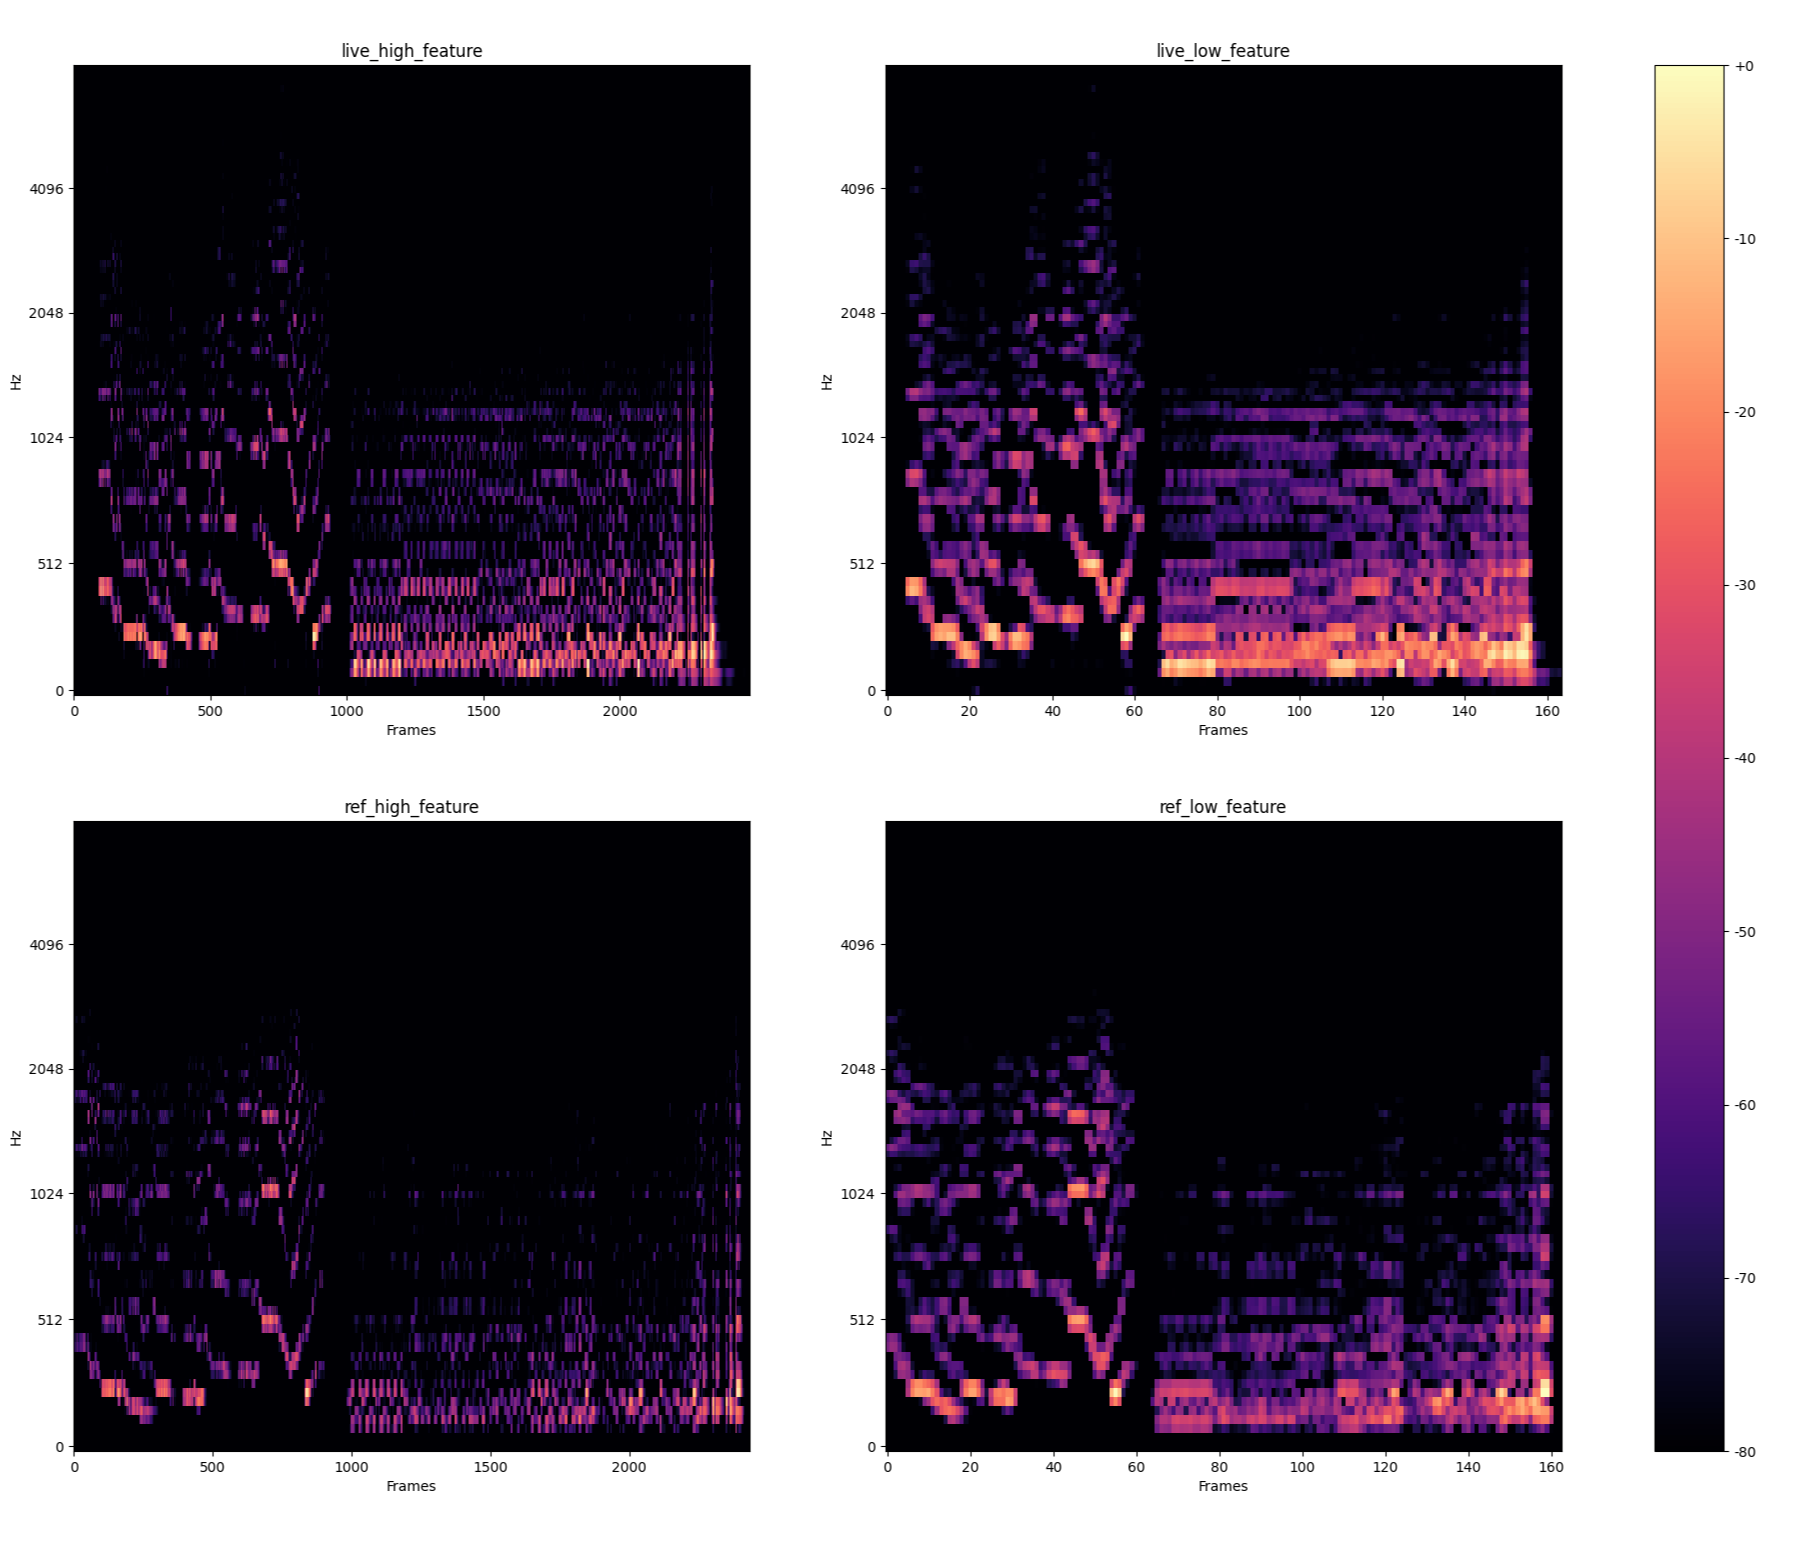
\includegraphics[width=\linewidth]{ch3/fig-feature.png}
    \caption{上:現場音訊的高(左) / 低(右)解析度特徵圖;下:參考音訊的高(左) / 低(右)解析度特徵圖}
    \label{fig:fig-ch3-feature}
\end{figure}

\subsection{Music Detector Block} \label{ch3-subst-music-detector}
Music Detector為負責偵測使用者開始演奏的時間並觸發後面元件啟動的process,
我們實作了平均振幅的閥值判斷並參考~\cite{Lin2020AHumanComputerDuetSystem}
的DTW對齊成本閥值判斷方法來實現。

當Music Detector接收到音訊時,
我們計算平均振幅並根據事先定義的閥值$\theta _{A}$判斷此片段是否為靜音片段,
振幅平均值的計算公式如\cref{eq:avarage-amplitude-function}所示,
$N$為整段音訊的樣本數,$| x[n] \vert$為音訊第n個樣本的絕對值,
A為振幅平均值。
\begin{equation}
    \label{eq:avarage-amplitude-function}
    A = \frac{1}{N} \sum _{n=1}^{N} | x[n] \vert 
\end{equation}
$\theta _{A}$的值是透過統計的方式來決定設定的值,
我們使用已標記音樂開始時間的音訊來一一測試,
已標記的音訊是使用自己錄製的音檔來測試,
我們透過測量每一首的音樂開始時間的振幅值與音樂尚未開始時間的振幅值,
並將音樂開始時間的振幅值加總後取平均獲得,最後我們將$\theta _{A}$設為0.01。

\cref{eq:amplitude-threshold-cases}為平均振幅與閥值的條件判斷公式,
當$A \leq \theta _{A}$時,代表此片段為靜音片段,因此直接回頭計算新的音訊的平均振幅,
當$A > \theta _{A}$時,代表此片段為非靜音片段,可能為音樂開始的地方,
因此將此片段接著使用DTW對齊成本閥值判斷方法。

\begin{equation} 
    \label{eq:amplitude-threshold-cases}
    \begin{cases}
        \text{Compute DTW cost}, & \text{if $A > \theta _{A}$} \\
        \text{Do nothing},  & \text{if $A \leq \theta _{A}$}
    \end{cases}
\end{equation}

DTW對齊成本閥值判斷方法我們參考~\cite{Lin2020AHumanComputerDuetSystem}
,當現場音訊通過平均振幅閥值的判斷後,
我們將音訊擷取為高解析度特徵並與參考音訊開頭0.5秒的高解析度特徵
計算DTW對齊成本${DTW_{cost}}$。
若${DTW_{cost}}$小於設定好的閥值$\theta _{cost}$,
Music Detector就會觸發tracking event。
$\theta _{cost}$的值與上述提到$\theta _{A}$的設定方法一樣為統計的方式,
我們將$\theta _{cost}$設為2000。

\cref{eq:DTW-cost-threshold-cases}為DTW對齊成本與閥值的條件判斷公式,
當$DTW_{cost} \geq \theta _{cost}$時,認定此兩段音訊的相似度不足,
因此不觸發後面的元件並回頭計算新的音訊的平均振幅,
當$DTW_{cost}  < \theta _{cost}$時,認定此兩段音訊具有足夠的相似度被認定為音樂開始的片段,
因此觸發後面的元件並關閉自己的process。
\begin{equation}
    \label{eq:DTW-cost-threshold-cases}
    \begin{cases}
        \text{Trigger tracking event}, & \text{if $DTW_{cost} < \theta _{cost}$} \\
        \text{Do nothing}, & \text{if $DTW_{cost} \geq \theta _{cost}$}
    \end{cases}
\end{equation}

\subsection{Rough Position Estimator Block} \label{ch3-subst-RPE}
在追蹤系統啟動後,為了避免Decision Maker的錯誤對齊,
Rough Position Estimator (RPE) 負責使用低解析度特徵計算
目前最新現場音訊幀與參考音訊每一幀的相似度,
並挑出相似度高的前8個粗略估計位置提供給Decision Maker參考。

當新的音訊幀經過特徵擷取後,
RPE會獲得新的現場低解析度特徵$Live_{low}[t] \in \mathbb{R}^{1 \times F}$,
$t$為最新的低解析度特徵時間點。
此時RPE計算$Live_{low}[t]$與整個參考低解析度特徵$Ref_{low} \in \mathbb{R}^{N \times F}$
的歐基里德距離並紀錄到距離成本矩陣$D_{RPE} \in \mathbb{R}^{t \times N}$,
$N$為$Ref_{low}$的時間長度。
\cref{eq:RPE-Distance-cost-function}
表示在現場與參考的時間點為$[t, n]$時兩個低解析度特徵的距離。
\cref{fig:fig-ch3-RPE-cost-matrix}為實際計算出來的$D_{RPE}$,
越亮的地方代表兩格特徵距離越遠。
\begin{equation}
    \label{eq:RPE-Distance-cost-function}
    D_{RPE}[t, n] = \sum_{f = 0}^{F}\sqrt{
    \left\lvert Ref_{low}[n, f]-Live_{low}[t, f]\right\rvert^{2}} 
\end{equation}

\begin{figure}[H]
    \centering
    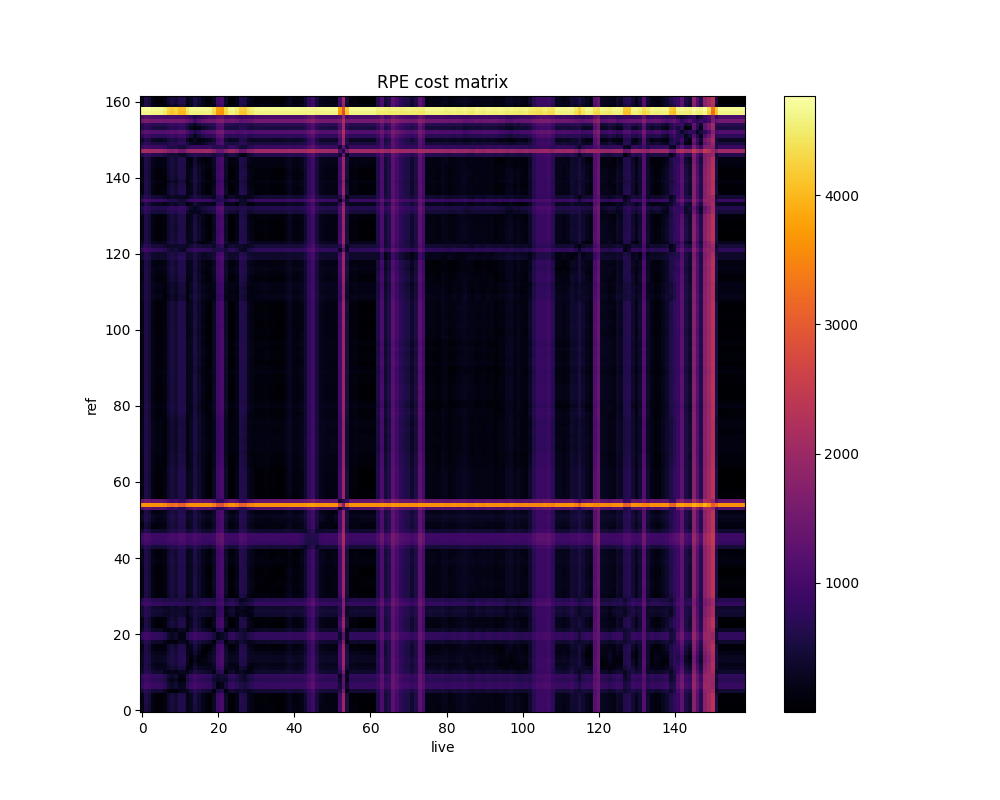
\includegraphics[width=\linewidth]{ch3/fig-RPE-cost-matrix.png}
    \caption{RPE 距離矩陣}
    \label{fig:fig-ch3-RPE-cost-matrix}
\end{figure}

當$D_{RPE}$累積現場9秒($\sim 30$\ low feature frames)的資訊後,
使用GBA方法計算時間點$t$時$Ref_{low}$
所有時間點向後對齊9秒的最小路徑成本矩陣$C_{RPE} \in \mathbb{R}^{1 \times N}$,
我們將RPE的$GBA_{Max\_Run}$設定為3,
當最小路徑成本值越小,代表此參考點與目前現場位置的相似度越高,
因此我們對$C_{RPE}$做Min-Max資料正規化,公式如\cref{eq:RPE-Min-Max-normalization-function}所示,
所有最小成本路徑值都被正規化到$[0,1]$之間,
並且相似度高的值越接近$1$。
\begin{equation}
    \label{eq:RPE-Min-Max-normalization-function}
    S_{RPE} = 1-\frac{C_{RPE}[n]-min(C_{RPE})}{max(C_{RPE})-min(C_{RPE})},
    n = \left\{0, 1 \ldots N\right\} 
\end{equation}

最後我們獲得相似度矩陣$S_{RPE} \in \mathbb{R}^{1 \times N}$,
為了取出前8個相似度最高的估計位置,
我們對$S_{RPE}$進行降冪排序,並且設定了一個相似度閥值$\theta _{S}$,
當$S_{RPE}$中的值超過$\theta _{S}$且排序在前8個順序時,
才可以做為粗略估計位置輸出給Decision Maker,
我們參考~\cite{Arzt2010Towards}的設定,將為$\theta _{S}$設為0.95。
另外累積超過9秒的現場音訊後,
下一次的GBA方法計算會在1.5秒($\sim 5$\ low feature frames)後,
這是為了節省計算資源,使系統能保持在即時的狀態。
RPE的粗略估計位置點如\cref{fig:fig-ch3-RPE-cost-matrix-with-output}的白色點所示。
\begin{figure}[H]
    \centering
    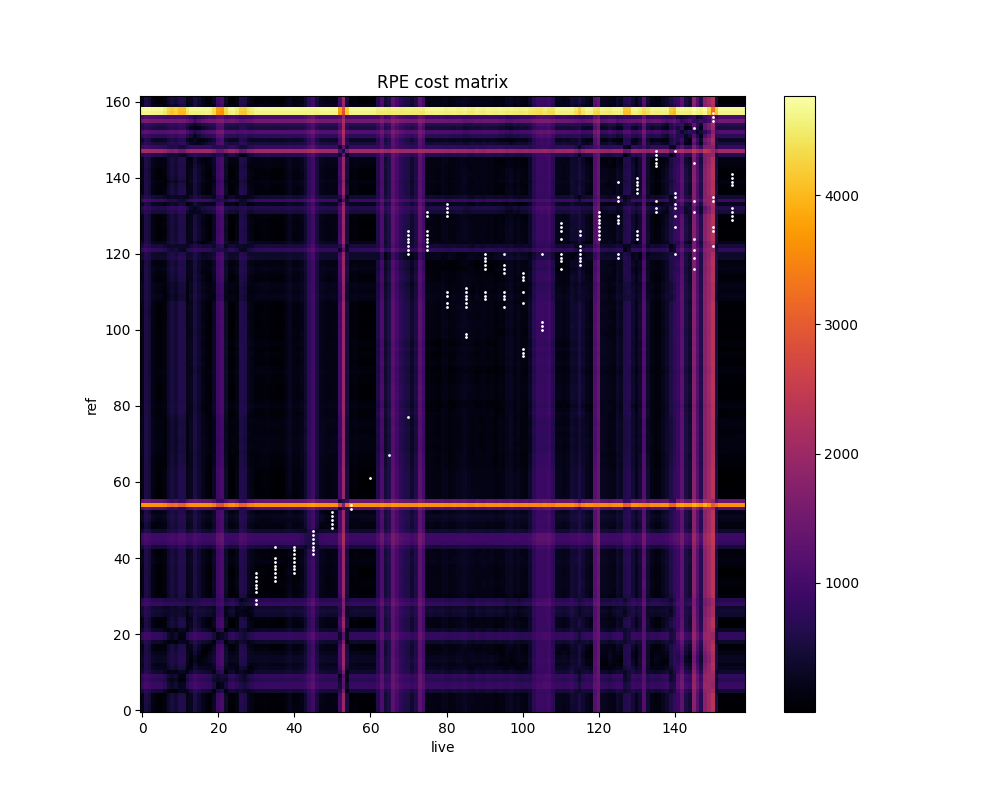
\includegraphics[width=\linewidth]{ch3/fig-RPE-cost-matrix-with-output.png}
    \caption{RPE 粗略估計位置}
    \label{fig:fig-ch3-RPE-cost-matrix-with-output}
\end{figure}

% 使用低解析度特徵、
% 如何計算cost matrix、
% Greedy的設置與做法(在前面解釋)、
% 決定輸出的機制、
% 放圖

\subsection{Decision Maker Block} \label{ch3-subst-decision-maker}
Decision Maker由ODTW thread與GBA threads所組成,
負責即時計算現場高解析度特徵與參考高解析度特徵的即時對齊位置,
並參考RPE的粗略估計位置決定最後輸出,
為此音樂追蹤模組中最重要的區塊。

在ODTW thread中會持續接收現場高解析度特徵$Live_{high}[t] \in \mathbb{R}^{1 \times F}$
,並與參考高解析度特徵$Ref_{high} \in \mathbb{R}^{N \times F}$
計算兩種距離矩陣$D_{cell} \in \mathbb{R}^{t \times N}$與
$D_{total} \in \mathbb{R}^{t \times N}$,
ODTW的計算方式與參數設定如\ref{ch3-subst-ODTW}節所示,
若目前沒有RPE的粗略估計位置加入,則輸出ODTW所計算出來的對齊位置。

GBA threads會接收來自RPE所計算出來的粗略估計位置
並使用ODTW的距離成本矩陣$D_{total}$計算GBA結果,
為了不讓RPE完全控制輸出結果,
我們將目前ODTW計算出來的輸出位置$output_j$
與$(output_j\pm 15, 30, 45)$一併加入GBA threads計算最終輸出位置。
我們將$GBA_{t}$設為15秒($\sim 750$\ high feature frames),
每個預計輸出位置將會向後計算15秒的最小路徑成本並選出成本最小的位置作為最後輸出。

\cref{fig:fig-ch3-desicion-maker-output}為ODTW的累積距離成本圖與Decision Maker的輸出路徑,
我們也將RPE的粗略估計位置(黃色點)結果與ODTW加入預計輸出的位置(桃紅色點)顯示在上面。
為了瞭解Decision Maker輸出的路徑是否有偏差,我們將DTW的輸出路徑(淺藍)呈現在
\cref{fig:fig-ch3-offline-and-online-path},並將Decision Maker輸出路徑(綠色)疊加在上面,
可以看到幾乎是與DTW的路徑重疊,代表此系統在即時對齊的能力與DTW離線對齊的能力相當。
\begin{figure}[H]
    \centering
    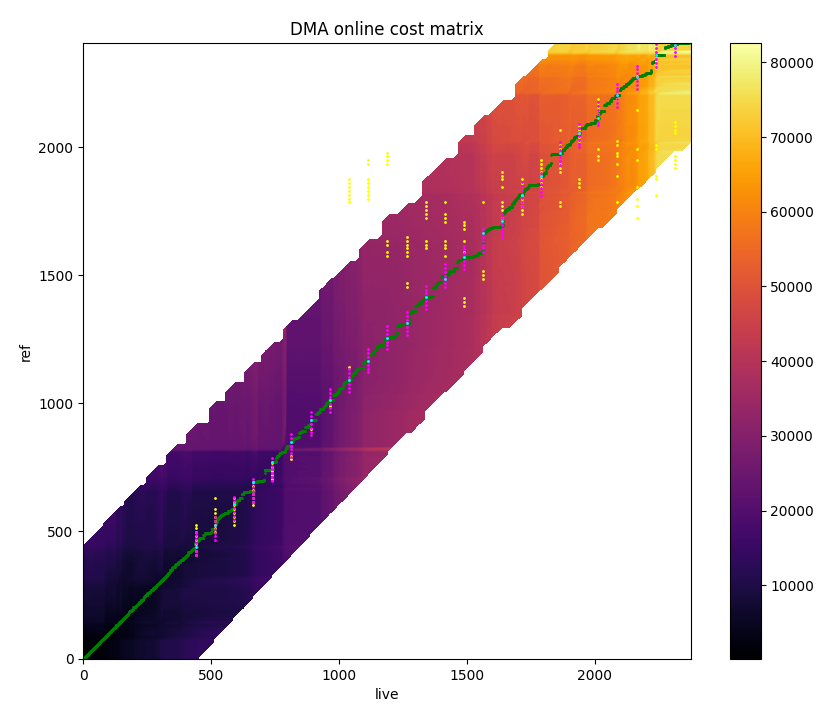
\includegraphics[width=0.8\linewidth]{ch3/fig-desicion-maker-output.png}
    \caption{Decision Maker計算的輸出點:\ 淺藍:GBA計算的最後輸出位置\ 綠色:ODTW計算的最後輸出位置}
    \label{fig:fig-ch3-desicion-maker-output}
\end{figure}
\begin{figure}[H]
    \centering
    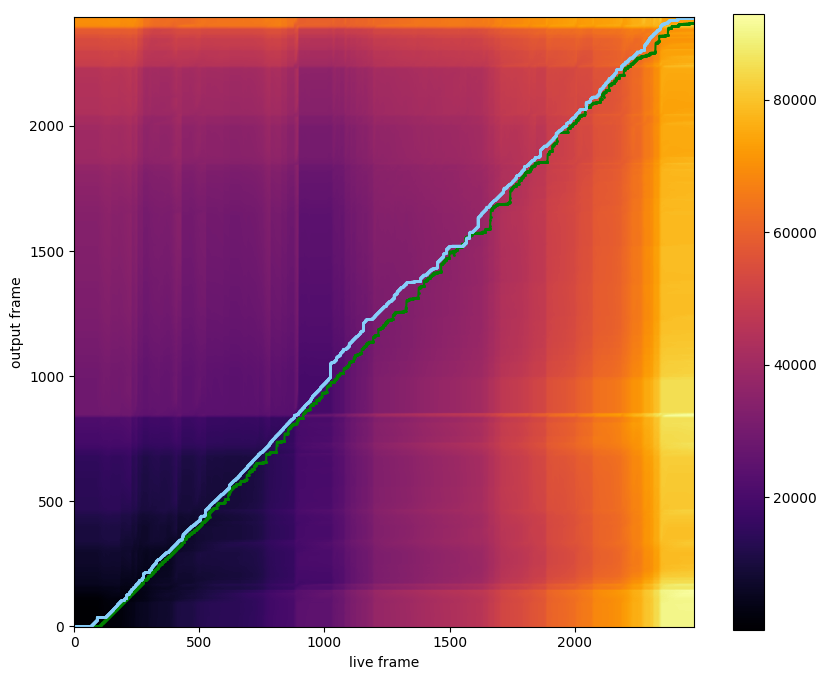
\includegraphics[width=0.8\linewidth]{ch3/fig-offline-and-online-path.png}
    \caption{DTW與音樂追蹤模組的輸出路徑比較圖}
    \label{fig:fig-ch3-offline-and-online-path}
\end{figure}

% 使用高解析度特徵、
% cost matrix的計算
% 清楚解釋ODTW main thread、
% 清楚解釋Greedy threads、
% 清楚解釋輸出的轉換
% 放圖

\pagebreak

\end{document}          % 研究方法
        \documentclass[class=NCU_thesis, crop=false]{standalone}
\begin{document}

\chapter{實驗設計與結果}

\section{音源分離評估}
本節將比較兩個不同的音源分離模型,Aug4mss~\cite{Chiu_ChingYu2020MixingSpecific}
與本研究使用的Band-Split RNN~\cite{Luo_Yi2022MusicSourceSeparation}
在小提琴與鋼琴混合音訊資料上的表現。首先介紹使用的訓練資料集與測試資料集,
接著介紹模型訓練的設定、評估指標與評估結果。

\subsection{音源分離資料集}
在眾多的音訊公開資料集中,能同時包含多音軌錄音資料和乾淨的單音軌錄音資料可說是少之又少,
在古典樂器的音訊資料集更是如此。
Aug4mss從網路上蒐集了
6小時的古典小提琴獨奏錄音與6小時的流行鋼琴獨奏錄音作為他們的訓練與驗證資料集,
但因為版權的關係,他們並沒有提供資料集給外界使用。
因此本研究遵循Aug4mss蒐集資料集的方式,
將小提琴與鋼琴兩種樂器的資料分開蒐集。
我們整合了多個公開資料集作為訓練資料,公開資料集包含由John Thickstun等人提供的
MusicNet~\cite{Thickstun2017Learning, Thickstun2018Invariances}、
Muneratti Ortega等人提供的Expressive Solo Violin~\cite{Muneratti_Ortega2021Expressive}與
Dong, Hao-Wen等人提供的Bach Violin Dataset~\cite{Dong_HaoWen2021Bach}。

MusicNet資料集中有330個古典音樂錄音,
錄音種類包含鋼琴獨奏、小提琴獨奏、大提琴獨奏、長笛獨奏、鋼琴與樂器合奏、管樂合奏與弦樂合奏等組合,
我們從資料集中挑選出鋼琴獨奏與小提琴獨奏的錄音資料作為訓練資料集的一部分。
Expressive Solo Violin資料集是由專業的小提琴家在同一天錄製九個不同曲子片段的錄音,
每一個片段會以不同的音樂表達方式演奏三次,並使用多個電容式麥克風同時錄音。
我們採用了資料集中所有的錄音資料(81個片段)作為訓練資料集的一部分。
Bach Violin Dataset為整合了高品質公開錄音的巴赫小提琴獨奏奏鳴曲(BWV 1001-1006)資料集,
其中包含17位小提琴家在不同的演奏場所下錄製的資料,
我們採用有提供錄音檔案的資料作為訓練資料集的一部分。

整合完畢的訓練資料集格式如\cref{table:table-ours-training-dataset}所示,
小提琴獨奏音檔的總時長為5小時24分47秒,
鋼琴獨奏音檔的總時長為5小時06分37秒,
所有資料皆為單聲道WAVE音訊格式。
\begin{table}[h]
    \centering
    \caption{整合的訓練資料集格式}
    \label{table:table-ours-training-dataset}
    \begin{tabular}{|c|c|c|}
        \hline
        \multicolumn{1}{|c|}{} & \multicolumn{1}{|c|}{小提琴音源} & \multicolumn{1}{|c|}{鋼琴音源} \\
        \hline
        總時長 & 5hr 24min 47sec & 5hr 6min 37sec \\
        \hline
        Channel & Mono & Mono \\
        \hline
        音訊格式 & WAV & WAV \\
        \hline
    \end{tabular}
\end{table}

我們根據~\cite{Chiu_ChingYu2020MixingSpecific}中切割資料集的方式,
將每種樂器的訓練資料集切成訓練集與驗證集,如\cref{table:table-ours-splited-dataset}所示。
\begin{table}[h]
    \centering
    \caption{每種樂器的訓練集與驗證集大小}
    \label{table:table-ours-splited-dataset}
    \begin{tabular}{|c|c|c|}
        \hline
        \multicolumn{1}{|c|}{} & \multicolumn{1}{|c|}{小提琴} & \multicolumn{1}{|c|}{鋼琴} \\
        \hline
        訓練集 & 4hr & 4hr \\
        \hline
        驗證集 & 1hr 6min 37sec & 1hr 24min 47sec\\
        \hline
    \end{tabular}
\end{table}

測試資料集我們採用Aug4mss
提供的公開整合測試資料集進行評估,
此資料集是從公開資料集MedleyDB~\cite{Bittner2014MedleyDB}中特別
挑選出小提琴與鋼琴的錄音所製作的測試資料集。

% \colorbox{yellow}{放資料集的連結?}

\subsection{模型訓練細節} \label{training-dataset-processing}
為了公平起見,我們使用自己的公開資料集重新訓練Aug4mss模型來評估效能,
在Aug4mss的論文~\cite{Chiu_ChingYu2020MixingSpecific}中
透過控制每次迭帶的訓練樣本數設計了Data-limit與Data-rich兩種情境,
測試模型在資料缺乏與資料足夠時的表現。
因此在訓練兩種模型時,
我們參考~\cite{Chiu_ChingYu2020MixingSpecific}設定的資料筆數$N$,
$N$為在模型訓練過程中,每次迭帶從每種樂器的資料集隨機選取$N$對所混合的資料筆數,
每對資料皆為10秒鐘的混合音訊。
我們將針對上述兩種情況做測試。
訓練與驗證的資料筆數$N$如\cref{table:table-training-dataset-split}所示,
random seed皆設定為42,確保兩個模型訓練時所拿到的資料為一致的。
\begin{table}[h]
    \centering
    \caption{每次迭帶的訓練與驗證資料筆數}
    \label{table:table-training-dataset-split}
    \begin{tabular}{|c|c|c|}
        \hline
        \multicolumn{1}{|c|}{} & \multicolumn{1}{|c|}{Data-limit} & \multicolumn{1}{|c|}{Data-rich} \\
        \hline
        \textbf{訓練}資料混合筆數 & 250 pairs & 2000 pairs \\
        \hline
        \textbf{驗證}資料混合筆數 & \multicolumn{2}{|c|}{100 pairs} \\
        \hline
    \end{tabular}
\end{table}

所有訓練與測試的資料皆為44100Hz取樣率的單聲道音訊,
特徵採樣參數STFT Window size為2048,Hop size為512,並保留原始模型的設定參數。
模型訓練所使用的顯示卡為GeForce RTX™ 3080 Ti,
CPU為11th Gen Intel(R) Core(TM) i7-11700K @ 3.60GHz。

\subsection{音源分離評估指標}
我們使用~\cite{Luo_Yi2022MusicSourceSeparation}中的兩種評估指標來評估模型,
這兩種評估指標皆是基於\cref{eq:SDR-function}計算訊號失真比(Signal-to-Noise Ratio, SDR)。
\begin{equation}
    \label{eq:SDR-function}
    SDR = 10\log _{10}
    \frac{\sum _{n}\left\lVert s(n)\right\rVert^{2} + \epsilon }
    {\sum _{n}\left\lVert s(n)-\hat{s}(n) \right\rVert^{2} + \epsilon}, s(n)\in \mathbb{R}^{2}
\end{equation}
上述公式計算同一筆資料中在離散時間$n$的訊號失真比,
$s(n)$為正確的波型,$\hat{s}(n)$為估計的波型,
另外為了避免除數為零,我們使用一個很小的常數$\epsilon = 10^{-7}$來避免這個情況。
當SDR的值越高,代表估計的波型與正確的波型越相近,分離效果越好。

下面介紹兩種評估指標的來源與計算方法:
\begin{enumerate}
    \item uSDR:Utterance-level SDR為~\cite{Yuki_Mitsufuji2021MusicDemixing}
    提出的評估方法,我們使用官方的版本針對整個訊號來計算SDR,並計算所有曲子的平均SDR數值。
    \item cSDR:Chunk-level SDR為bss\_eval指標~\cite{Vincent2006Performance}
    中計算的SDR方法,我們使用官方的版本,計算每首曲子中所有1秒區塊的SDR中位數,
    獲得每首曲子的SDR數值後再取中位數。
\end{enumerate}

% 最後將小提琴與鋼琴的SDR加總取平均

% \begin{equation}
%     \label{eq:SDR-song-function}
%     SDR_{Songs} = \frac{1}{2} (SDR_{Violin} + SDR_{Piano})
% \end{equation}

\subsection{音源分離結果比較}

根據 \ref{training-dataset-processing} 節所提到的兩種情況,
\cref{table:table-data-limit-music-source-separation}
與\cref{table:table-data-rich-music-source-separation}
為模型在Data-limit與Data-rich情況下訓練的結果。

另外,Aug4mss\cite{Chiu_ChingYu2020MixingSpecific}加入了多種
Data Augmentation方法測試模型效能,
由於本研究在訓練模型時皆採用相同的隨機混合方式,
因此本研究只比較~\cite{Chiu_ChingYu2020MixingSpecific}中Random mixing的結果。

\begin{table}[h]
    \centering
    \caption{Data-limit 結果數值比較}
    \label{table:table-data-limit-music-source-separation}
    \begin{tabular}{|c|c|c|c|}
        \hline
        \multicolumn{1}{|c|}{分離目標樂器} & \multicolumn{1}{|c|}{模型} & \multicolumn{1}{|c|}{cSDR} & \multicolumn{1}{|c|}{uSDR}\\
        \hline
        \multirow{3}*{Violin} & Aug4mss(paper) & 1.08 & N/A \\
        \cline{2-4}
        ~ & Aug4mss(retrain) & 2.05 & 1.72 \\
        \cline{2-4}
        % ~ & \textbf{Band-Split RNN} & \textbf{8.910} & \textbf{3.264} \\
        ~ & \textbf{Band-Split RNN} & \textbf{8.085} & \textbf{5.580} \\
        \hline
        \multirow{3}*{Piano} & Aug4mss(paper) & 7.43 & N/A \\
        \cline{2-4}
        ~ & Aug4mss(retrain) & 11.906 & 10.974 \\
        \cline{2-4}
        % ~ & \textbf{Band-Split RNN} & \textbf{14.659} & \textbf{13.460} \\
        ~ & \textbf{Band-Split RNN} & \textbf{15.975} & \textbf{14.854} \\
        \hline
    \end{tabular}
\end{table}

\begin{table}[h]
    \centering
    \caption{Data-rich 結果數值比較}
    \label{table:table-data-rich-music-source-separation}
    \begin{tabular}{|c|c|c|c|}
        \hline
        \multicolumn{1}{|c|}{分離目標樂器} & \multicolumn{1}{|c|}{模型} & \multicolumn{1}{|c|}{cSDR} & \multicolumn{1}{|c|}{uSDR}\\
        \hline
        \multirow{3}*{Violin} & Aug4mss(paper) & 3.84 & N/A \\
        \cline{2-4}
        ~ & Aug4mss(retrain) & 5.811 & 5.666 \\
        \cline{2-4}
        ~ & \textbf{Band-Split RNN} & \textbf{11.872} & \textbf{8.297} \\
        \hline
        \multirow{3}*{Piano} & Aug4mss(paper) & 13.46 & N/A \\
        \cline{2-4}
        ~ & Aug4mss(retrain) & 13.514 & 14.124 \\
        \cline{2-4}
        ~ & \textbf{Band-Split RNN} & \textbf{16.526} & \textbf{15.467} \\
        \hline
    \end{tabular}
\end{table}

在 Data-limit 的情況下,Band-Split RNN 在小提琴和鋼琴的分離效果上都是表現最為出色。
Band-Split RNN 在小提琴分離上的 cSDR 和 uSDR 分別為 8.085 和 5.580,
而在鋼琴分離上的 cSDR 和 uSDR 分別為 15.975 和 14.854。
相比之下,Aug4mss (retrain) 的結果分別為 2.05 和 1.72(小提琴),
以及 11.906 和 10.974(鋼琴)。

在 Data-rich 的情況下,Band-Split RNN 在小提琴和鋼琴的分離效果上也是表現最為出色。
Band-Split RNN 在小提琴分離上的 cSDR 和 uSDR 分別為 11.872 和 8.297,
而在鋼琴分離上的 cSDR 和 uSDR 分別為 16.526 和 15.467。
相比之下,Aug4mss (retrain) 的結果分別為 5.811 和 5.666(小提琴),
以及 13.514 和 14.124(鋼琴)。

可以注意到Aug4mss (retrain)的結果皆比Aug4mss (paper)要來的好,
可能是因為我們將原本的STFT參數改為與Band-Split RNN所設定的數值相同,
原本的Window Size從4096變為2048,Hop Size從1024改為512,因此使模型能訓練到更細部的特徵。

從\cref{table:table-data-limit-music-source-separation}與
\cref{table:table-data-rich-music-source-separation}可以看出,
不管是在資料缺少或是資料足夠的情況,Band-Split RNN皆在兩種分離目標中取得最好的數值,
我認為是因為Band-Split RNN有特別針對重要的頻帶做細部的切割,
使模型能學習到更重要的特徵。

\subsection{頻帶切割對於分離結果的影響}

在BSRNN~\cite{Luo_Yi2022MusicSourceSeparation}的論文中,
有針對頻帶分割模組對模型結果的影響做一系列的測試,
我們可以知道根據樂器不同的頻率範圍、音色特徵等等因素來調整頻帶分割的寬度,
可能會提升模型的結果。

在\ref{ch3-subst-estimate-band-split-point}節我們提出了頻帶切割估計方法並
針對不同的樂器設計不同的頻帶切割範圍,
為了驗證此方法效果,我們針對自己設計的頻帶切割範圍,實作以下三個實驗與音源分離結果比較,
\begin{enumerate}
    \item 使用~\cite{Luo_Yi2022MusicSourceSeparation}
    中效果最好的頻帶切割範圍V7訓練小提琴與鋼琴的音源分離模型
    \item 使用小提琴的頻帶切割範圍訓練鋼琴音源分離模型
    \item 使用鋼琴的頻帶切割範圍訓練小提琴音源分離模型
\end{enumerate}
V7、小提琴、鋼琴的子頻帶數皆為40個,
為了節省訓練時間,上述實驗皆使用Data-limit的情況訓練,
我們將這些模型的結果一一列出比較,
如\cref{table:table-data-limit-mss-band-split-range-comparision}所示。

\begin{table}[h]
    \centering
    \caption{Data-limit 不同的Band-Split Bandwidth結果比較}
    \label{table:table-data-limit-mss-band-split-range-comparision}
    \begin{tabular}{|c|c|c|c|}
        \hline
        \multicolumn{1}{|c|}{分離目標樂器} & \multicolumn{1}{|c|}{Bandwidth} & \multicolumn{1}{|c|}{cSDR} & \multicolumn{1}{|c|}{uSDR}\\
        \hline
        % \multirow{3}*{Violin} & \textbf{Violin bandwidth version} & \textbf{8.910} & \textbf{3.264} \\
        \multirow{3}*{Violin} & Violin bandwidth version & 8.085 & \textbf{5.580} \\
        \cline{2-4}
        % ~ & Piano bandwidth version & 8.796 & 3.077 \\
        ~ & Piano bandwidth version & \textbf{9.908} & 5.532 \\
        \cline{2-4}
        ~ & V7 bandwidth version & 8.842 & 3.157 \\
        \hline
        % \multirow{3}*{Piano} & Violin bandwidth version & 14.209 & 13.141 \\
        \multirow{3}*{Piano} & Violin bandwidth version & 15.653 & 14.851 \\
        \cline{2-4}
        % ~ & \textbf{Piano bandwidth version} & \textbf{14.659} & \textbf{13.460} \\
        ~ & Piano bandwidth version & \textbf{15.975} & \textbf{14.854} \\
        \cline{2-4}
        ~ & V7 bandwidth version & 14.556 & 13.370 \\
        \hline
    \end{tabular}
\end{table}

當目標樂器為小提琴時,我們使用小提琴的頻帶切割範圍的訓練結果雖然在cSDR指標並不是最高,
但在uSDR的表現上為最佳,優於使用鋼琴範圍與V7範圍的結果,
我認為可能是我們使用的估計頻帶資料多樣性太少,未來可以篩選不同曲風的小提琴音訊作為估計資料。
當目標樂器為鋼琴時,我們使用鋼琴的頻帶切割範圍的訓練結果優於使用小提琴範圍與V7範圍的結果,
由此可見,我們所提出的頻帶分割估計方法在uSDR的結果上皆優於BSRNN提出的V7頻帶範圍,
有助於提升音源分離的效果。

\pagebreak

\section{音樂追蹤評估}

\subsection{系統在不同速度下的追蹤結果} \label{ch4-subst-midi-tracking-results}
我們參考~\cite{Lin2020AHumanComputerDuetSystem}中的評估方法來檢測小提琴演奏追蹤系統的表現,
在~\cite{Lin2020AHumanComputerDuetSystem}中,現場演奏樂器為鋼琴,電腦輸出合奏為小提琴(MIDI),
參考音訊為MIDI檔案,
演奏曲子為貝多芬的Violin Sonata No.5, Op.24(Spring), movement I. Allegro 前25小節。
為了評估系統在不同演奏速度下的反應,他們使用四種不同速度範圍來測試系統,分別為演奏正常速度(115-145bpm)、
慢速(90-120bpm)、快速(135-175bpm)、漸快(由80bpm加速至160bpm),參考音訊的速度設定為120bpm。
他們使用錄音設備錄製現場鋼琴與小提琴的演奏,
並使用節拍追蹤工具得到現場與參考鋼琴之間的節拍位置,進一步生成正確小提琴輸出位置(Ground truth),
最後計算現場小提琴輸出位置與正確小提琴輸出位置的DTW對齊路徑,
使用\cref{eq:latency-function}與\cref{eq:avarage-latency-function}計算瞬間延遲與平均延遲來評估。

本研究使用的現場演奏樂器為小提琴,電腦輸出合奏為鋼琴,在演奏曲子與參考音訊速度的設定上我們跟隨
~\cite{Lin2020AHumanComputerDuetSystem}的設定,
然而在~\cite{Lin2020AHumanComputerDuetSystem}中並沒有提到他們是如何控制現場演奏速度的變化,
本研究為了能客觀地控制速度變化並計算評估結果,
我們將現場演奏的部分改為使用隨機生成速度的MIDI檔案來評估,
由於MIDI檔案擁有音符開始時間、節拍等等資訊,因此能精準地計算延遲,此外,
我們可以透過現場MIDI檔案生成正確的鋼琴輸出音訊,因此不需要額外的節拍追蹤工具輔助。
雖然現場演奏為預先設定好的檔案,但這並不影響即時的效果,現場音訊還是會以串流的方式進行處理。

\cref{fig:different-speed-midi-score-5bars}為在四種不同速度範圍下隨機生成的MIDI檔案,
我們透過讀取MIDI檔案中每個MIDI事件,將每個MIDI事件設定為有50\%的機率可以在速度範圍下隨機設定速度。
\cref{fig:slow-midi-5bars}為在慢速(90-120bpm)範圍的MIDI檔案、
\cref{fig:normal-midi-5bars}為在正常速度(115-145bpm)範圍的MIDI檔案、
\cref{fig:fast-midi-5bars}為在快速(135-175bpm)範圍的MIDI檔案,
可以看到每個有設定速度的MIDI事件,其速度設定都在對應的範圍中。
另外\cref{fig:accelerate-midi-5bars}為漸快(由80bpm加速至160bpm)範圍的MIDI檔案,
我們平均的將速度範圍分配到每個MIDI事件上,模擬漸快的情況。

\begin{figure}[H]
    %\captionsetup[subfigure]{labelformat=empty} % 完全隱藏圖號
    \centering
    \subcaptionbox
    {慢(90-120bpm)
    \label{fig:slow-midi-5bars}}
    {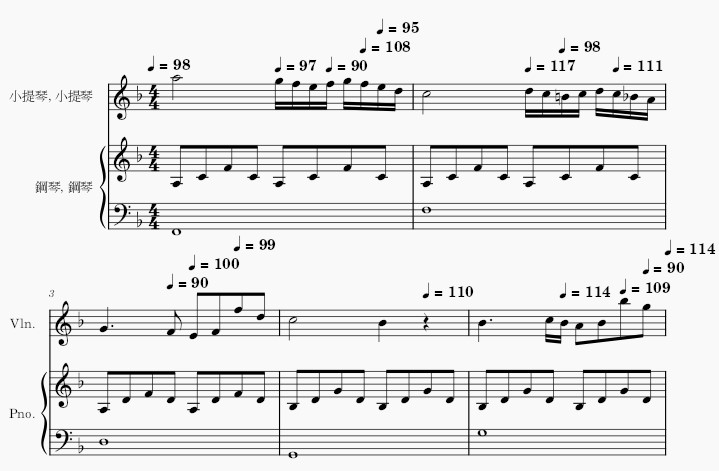
\includegraphics[width=0.4\linewidth, height=0.4\linewidth]{ch4/fig-midi-slow-score.jpg}}
    ~
    \subcaptionbox
    {一般(115-145bpm)
    \label{fig:normal-midi-5bars}}
    {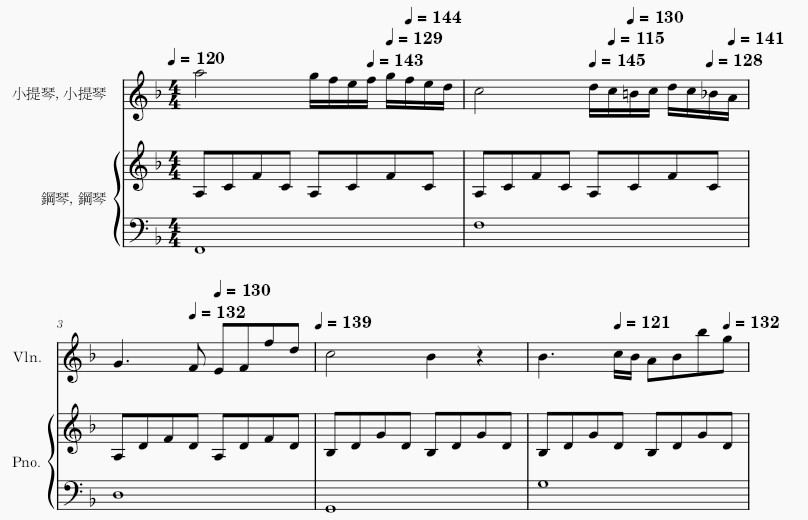
\includegraphics[width=0.4\linewidth, height=0.4\linewidth]{ch4/fig-midi-normal-score.jpg}}
    ~
    \subcaptionbox
    {快(135-175bpm)
    \label{fig:fast-midi-5bars}}
    {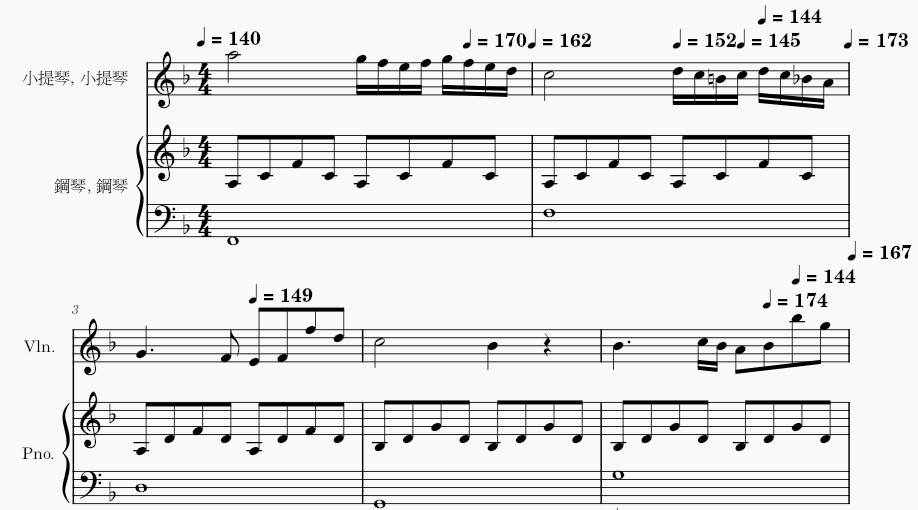
\includegraphics[width=0.4\linewidth, height=0.4\linewidth]{ch4/fig-midi-fast-score.jpg}}
    ~
    \subcaptionbox
    {加速(80$ \rightarrow $160bpm)
    \label{fig:accelerate-midi-5bars}}
    {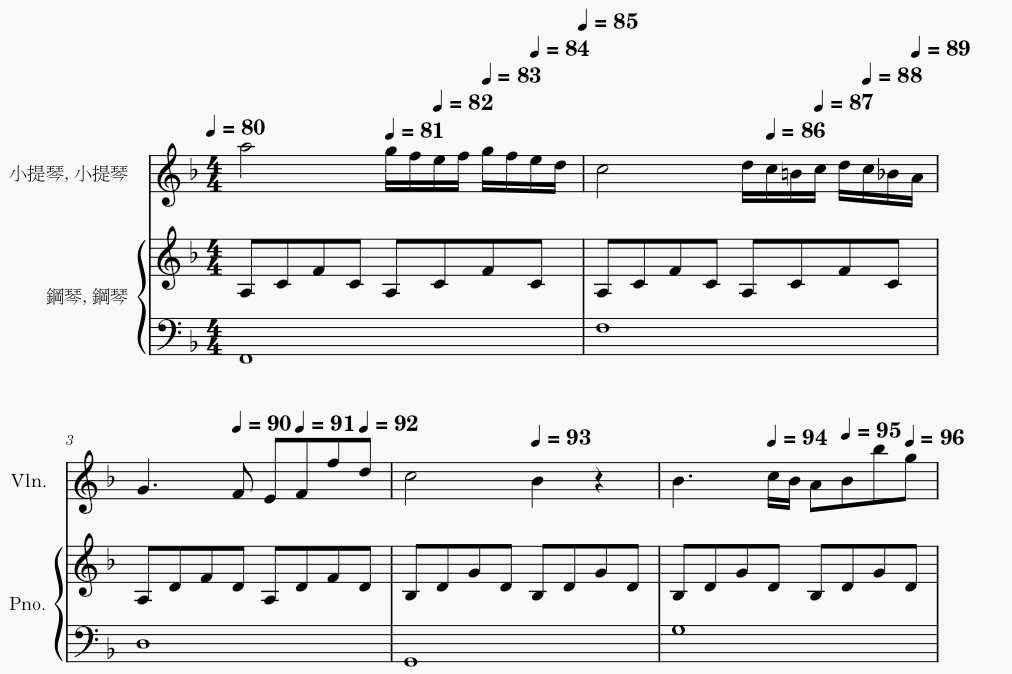
\includegraphics[width=0.4\linewidth, height=0.4\linewidth]{ch4/fig-midi-accelerate-score.jpg}}
    \caption{四種不同速度範圍的MIDI樂譜前五小節}
    \label{fig:different-speed-midi-score-5bars}
\end{figure}

由於正確的鋼琴輸出音訊已經透過MIDI檔案生成,
% 因此我們只需要使用追蹤結果與正確的鋼琴輸出音訊計算DTW對齊路徑,
我們只需要用正確伴奏音訊$Acc_{gt}$與追蹤系統估計的伴奏音訊$Acc_{out}$計算DTW對齊路徑,
由於伴奏音訊的時間長度是一致的,
因此可以根據\cref{eq:latency-function}
算出$Acc_{out}$在$Acc_{gt}$上的瞬間延遲(latency)。
\begin{equation}
    \label{eq:latency-function}
    \Delta [t_i] := t_j - t_i
\end{equation}

$t_i$為$Acc_{out}$的時間點,$t_j$為$Acc_{gt}$的時間點,
當$t_i = t_j$時,代表在這個時間點兩段音訊是對齊的,
當$t_i > t_j$時,代表$Acc_{out}$比$Acc_{gt}$還要快,
當$t_i < t_j$時,代表$Acc_{out}$比$Acc_{gt}$還要慢。

我們也用\cref{eq:avarage-latency-function}衡量整首曲子的平均延遲,
計算方式為將每個時間點的瞬間延遲取絕對值後加總,並除以曲子的長度$T$。
$| \Delta t\vert $為現場伴奏音訊的延遲。
\begin{equation}
    \label{eq:avarage-latency-function}
    \frac{1}{T} \sum _{t=0}^{T} | \Delta [t] \vert 
\end{equation}

\cref{fig:fig-ch4-slow-and-normal-latency-results}與\cref{fig:fig-ch4-fast-and-accelerate-latency-results}
顯示系統在四種速度變化下隨時間變化的延遲圖,也就是現場系統伴奏比正確伴奏要提前或落後多少個16分音符。
藍色線為系統延遲的16分音符數量,橘色線為當下的速度(bpm)。
\cref{fig:fig-slow-latency}是慢速時系統隨時間變化的延遲,可以看到系統在一開始雖然動盪較大,
但都保持在不超過2個16分音符的延遲下穩定追蹤,即使節拍動盪很大也不影響到系統的穩定性,
最後的平均延遲為55.04ms。
\cref{fig:fig-fast-latency}是快速時系統隨時間變化的延遲,
與慢速的延遲圖很像,但動盪較大,這可能是因為快速的速度範圍與參考的速度相差較多,
因此導致系統在追蹤時較容易有延遲,最後的平均延遲為62.96ms。
\cref{fig:fig-accelerate-latency}是漸快時系統隨時間變化的延遲,
由於一開始速度較慢,因此導致系統剛開始追蹤時動盪較大,當速度慢慢回升到接近參考音訊的速度時,
可以看到動盪越來越小,最後的平均延遲為58.23ms。
另外可以發現在第五小節(m5)與第七小節(m7)時,四種速度的延遲皆為正延遲,也就是比起正確的時間點還要提前,
可能是因為剛好那個時間點為休止符,也就是沒有音樂,因此造成系統先對齊到了最後面的靜音時間點並等待,
導致延遲。

\begin{figure}[H]
    %\captionsetup[subfigure]{labelformat=empty} % 完全隱藏圖號
    \centering
    \subcaptionbox
    {慢(90-120bpm) 平均延遲:55.04毫秒
    \label{fig:fig-slow-latency}}
    {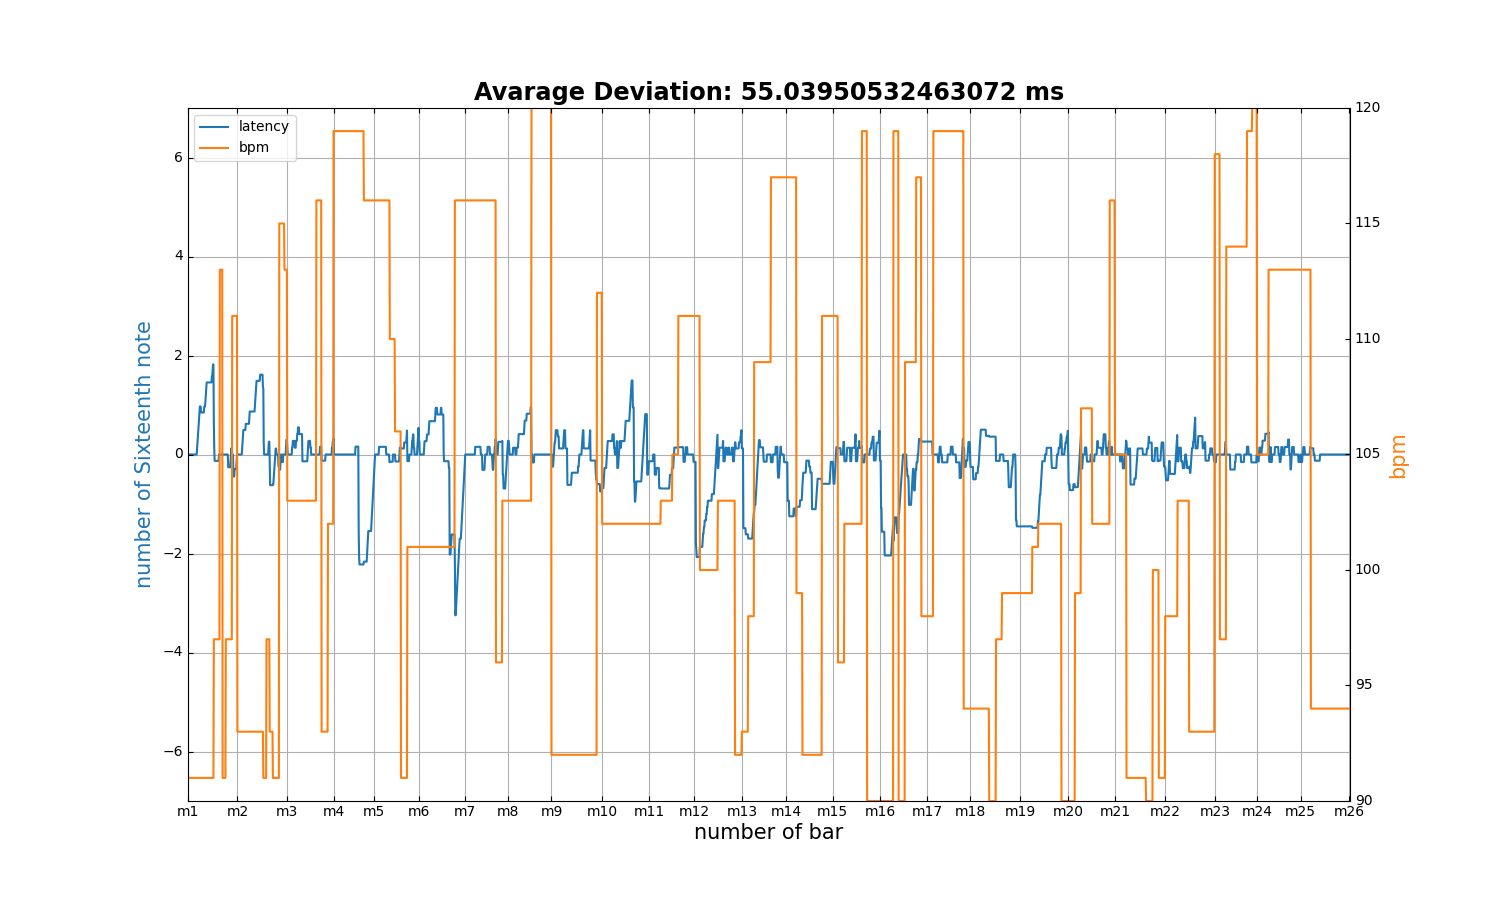
\includegraphics[width=\linewidth]{ch4/fig-slow-latency.png}}
    ~
    \subcaptionbox
    {一般(115-145bpm) 平均延遲:35.81毫秒
    \label{fig:fig-normal-latency}}
    {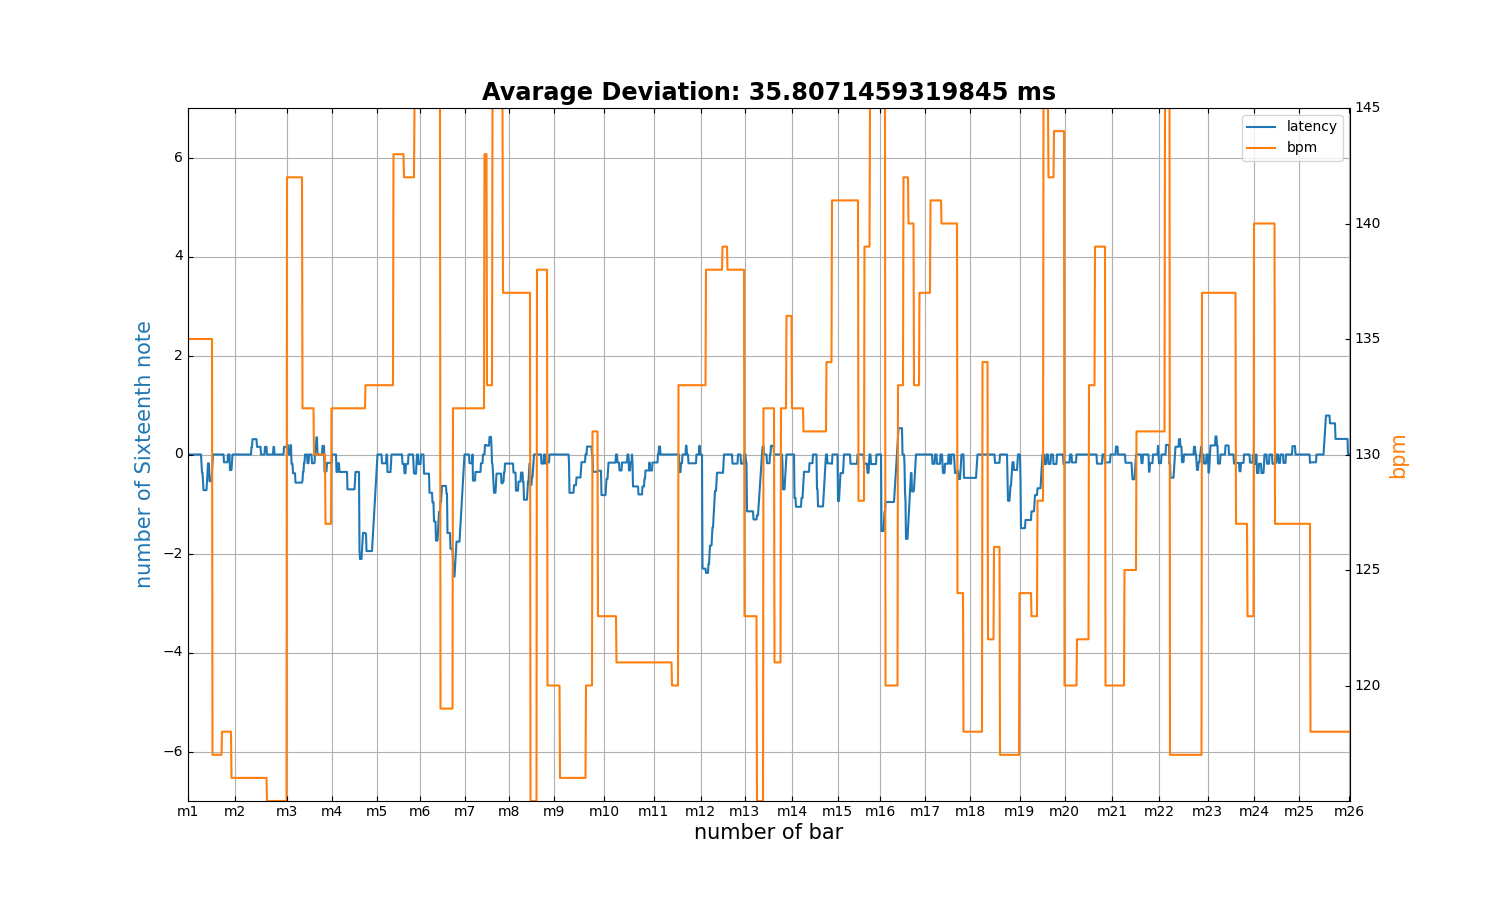
\includegraphics[width=\linewidth]{ch4/fig-normal-latency.png}}
    \caption{系統在慢、一般速度的延遲時間}
    \label{fig:fig-ch4-slow-and-normal-latency-results}
\end{figure}

\begin{figure}[H]
    %\captionsetup[subfigure]{labelformat=empty} % 完全隱藏圖號
    \centering
    \subcaptionbox
    {快(135-175bpm) 平均延遲:62.96毫秒
    \label{fig:fig-fast-latency}}
    {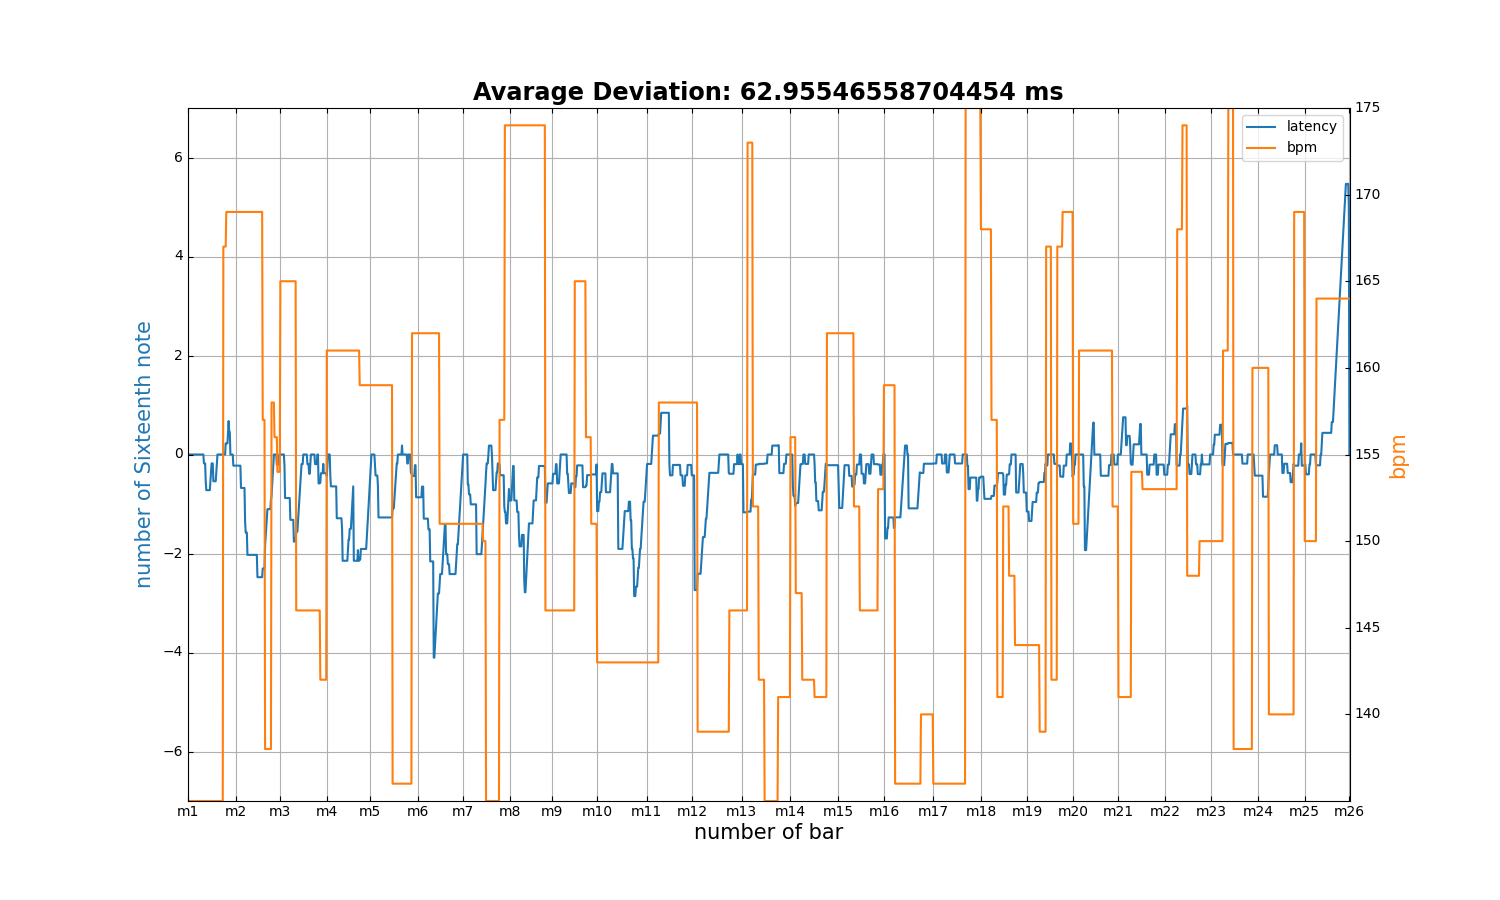
\includegraphics[width=\linewidth]{ch4/fig-fast-latency.png}}
    ~
    \subcaptionbox
    {加速(80$ \rightarrow $160bpm) 平均延遲:58.73毫秒
    \label{fig:fig-accelerate-latency}}
    {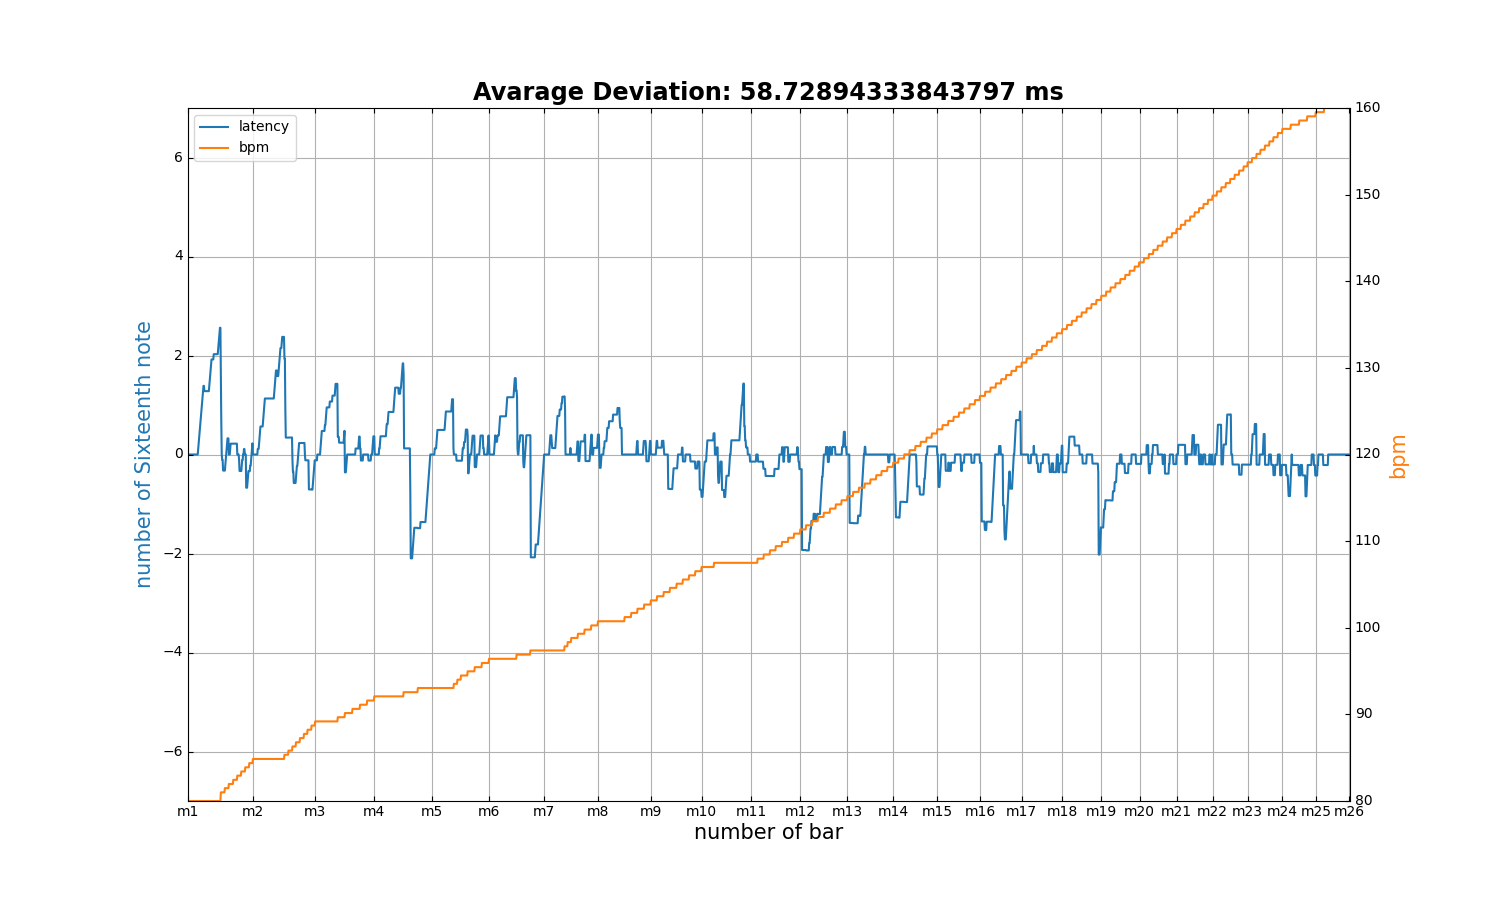
\includegraphics[width=\linewidth]{ch4/fig-accelerate-latency.png}}
    \caption{系統在快、加速速度的延遲時間}
    \label{fig:fig-ch4-fast-and-accelerate-latency-results}
\end{figure}


另外我們也顯示了四種速度的對齊路徑結果圖,橫軸為現場音訊的時間點,縱軸為參考音訊的時間點,
熱點圖的顏色代表在時間點$(i, j)$的累積距離成本值,成本值越高顏色越亮。
(a)圖為追蹤系統在執行時所輸出的結果圖,
(b)圖為離線對齊路徑與線上對齊路徑的比較圖,離線對齊路徑使用DTW計算。

\cref{fig:fig-ch4-slow-tracking-results}在大部分的時間點,速度會比參考音訊的速度要慢,
因此可以看到\cref{fig:slow-tracking-output}在某些區間(例如live約600frames時)
綠色的點所連成的線較為平緩,代表此區間系統輸出較多相同的參考音訊時間點來等待現場音訊。
在\cref{fig:slow-comparision-output}的表現上,幾乎與離線對齊時的最佳路徑是一致的。
% 只是可能系統上一些無法避免的延遲(例如接收串流音訊),造成兩條路徑並不是完整的重合。

\begin{figure}[H]
    %\captionsetup[subfigure]{labelformat=empty} % 完全隱藏圖號
    \centering
    \subcaptionbox
    {
    \label{fig:slow-tracking-output}}
    {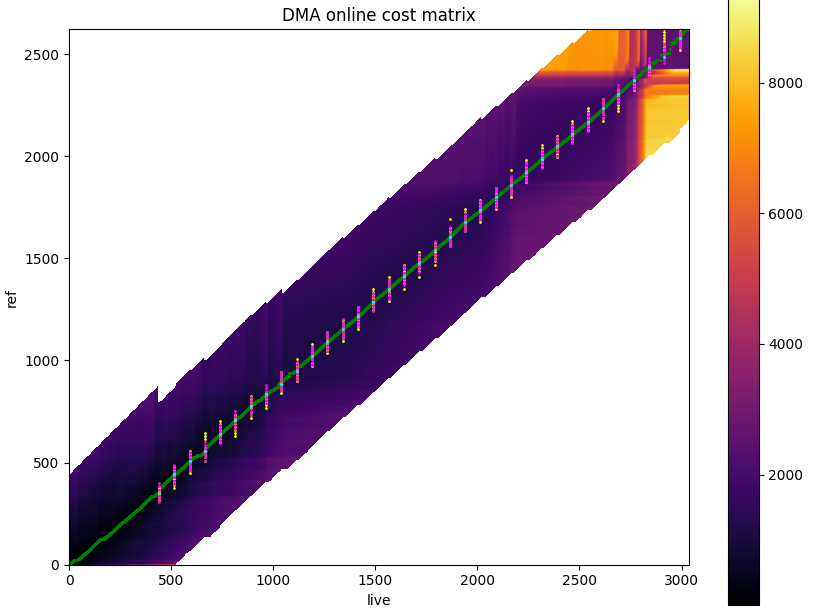
\includegraphics[scale=0.36]{ch4/fig-slow-tracking-system-output.png}}
    ~
    \subcaptionbox
    {
    \label{fig:slow-comparision-output}}
    {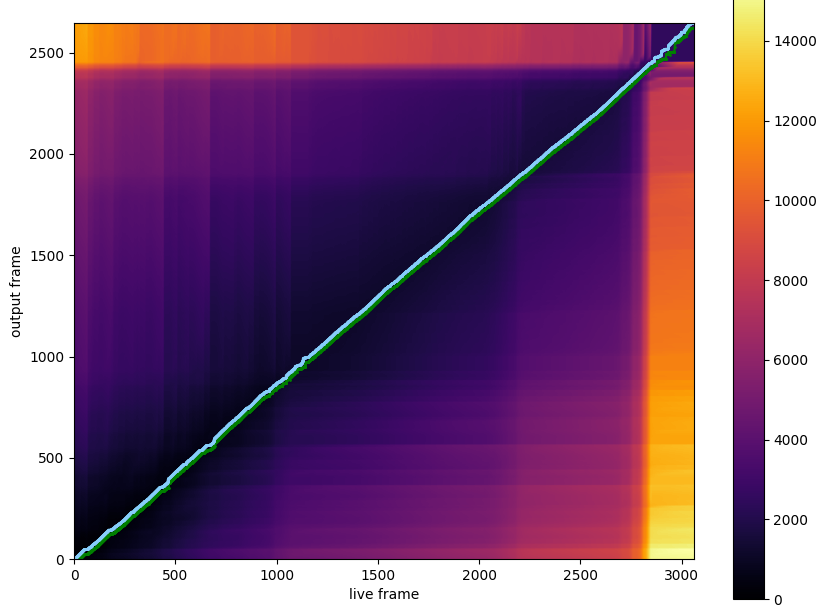
\includegraphics[scale=0.36]{ch4/fig-slow-offline-and-online-output.png}}
    \caption{慢(90-120bpm)}
    \label{fig:fig-ch4-slow-tracking-results}
\end{figure}

\cref{fig:fig-ch4-normal-tracking-results}的速度與參考音訊是最接近的,
因此在\cref{fig:normal-tracking-output}幾乎不會有波動,\cref{{fig:normal-comparision-output}}
也是表現得與離線對齊路徑相當。

\begin{figure}[H]
    %\captionsetup[subfigure]{labelformat=empty} % 完全隱藏圖號
    \centering
    \subcaptionbox
    {
    \label{fig:normal-tracking-output}}
    {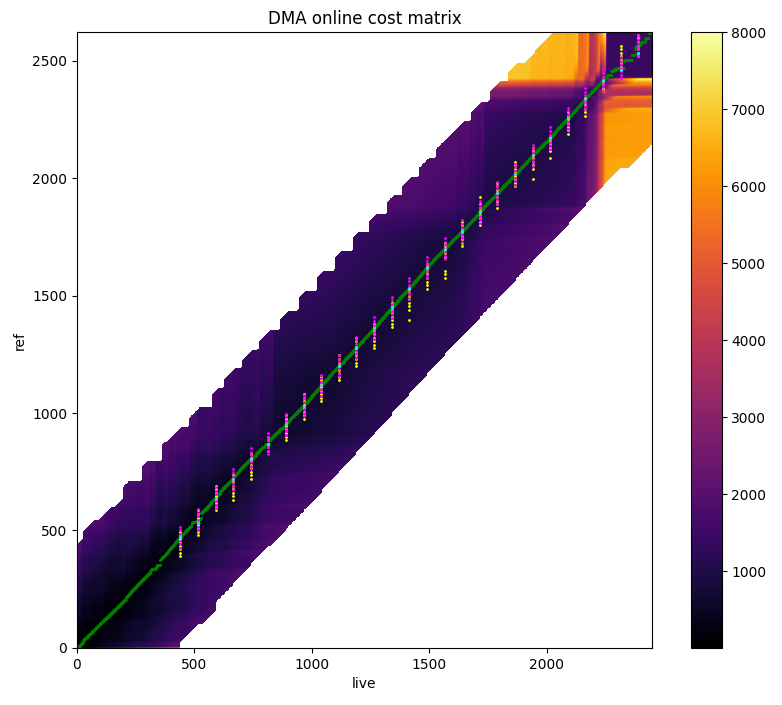
\includegraphics[scale=0.36]{ch4/fig-normal-tracking-system-output.png}}
    ~
    \subcaptionbox
    {
    \label{fig:normal-comparision-output}}
    {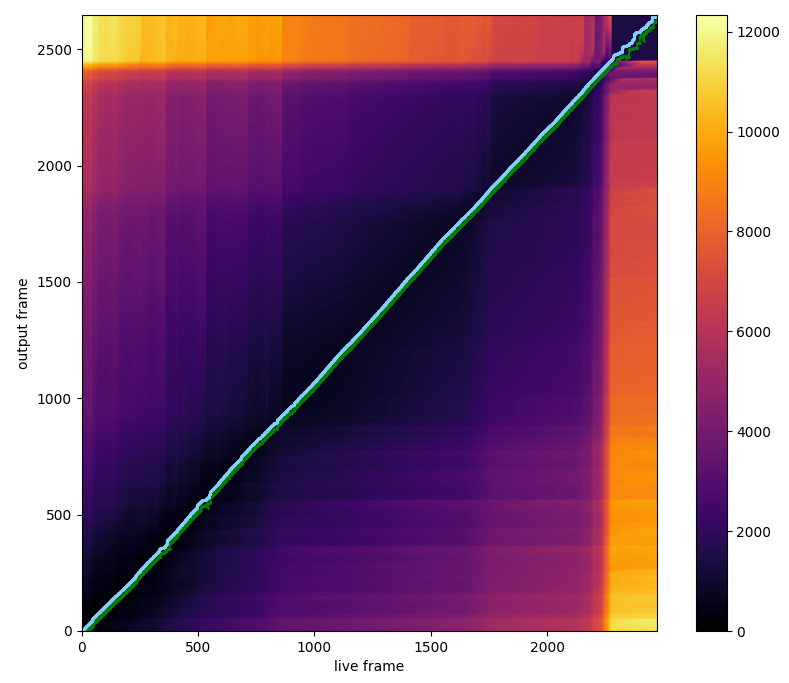
\includegraphics[scale=0.36]{ch4/fig-normal-offline-and-online-output.png}}
    \caption{一般(115-145bpm)}
    \label{fig:fig-ch4-normal-tracking-results}
\end{figure}

\cref{fig:fig-ch4-fast-tracking-results}在大部分的時間點,速度會比參考音訊的速度要快,
因此可以看到\cref{fig:fast-tracking-output}在某些區間(例如live約450frames時)
輸出路徑會呈現斷斷續續的點,代表此區間系統在輸出時認為目前現場音訊的時間點必須對齊到更後面的參考音訊,
在\cref{fig:fast-comparision-output}的表現上,雖然參考音訊的時間點並不是連續的,
但可以看到整體路徑與離線對齊路徑還是一致的。

\begin{figure}[H]
    %\captionsetup[subfigure]{labelformat=empty} % 完全隱藏圖號
    \centering
    \subcaptionbox
    {
    \label{fig:fast-tracking-output}}
    {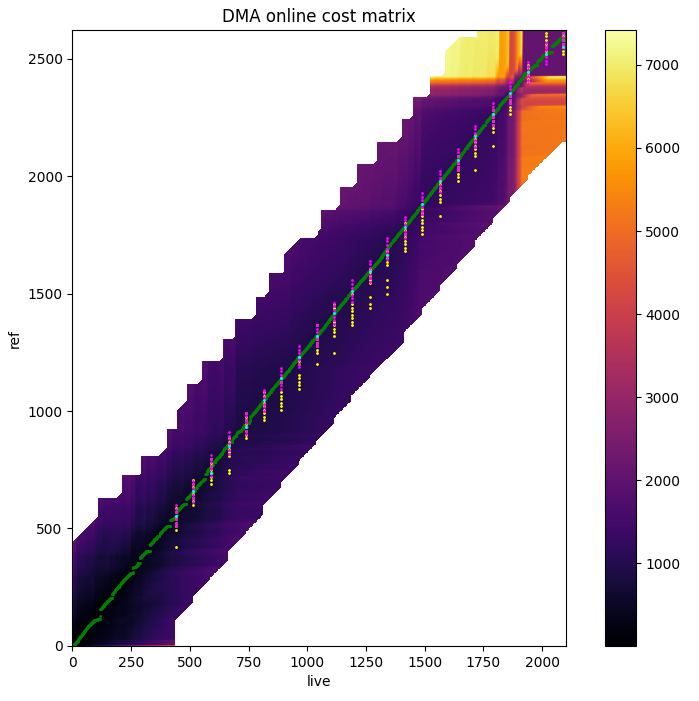
\includegraphics[scale=0.36]{ch4/fig-fast-tracking-system-output.png}}
    ~
    \subcaptionbox
    {
    \label{fig:fast-comparision-output}}
    {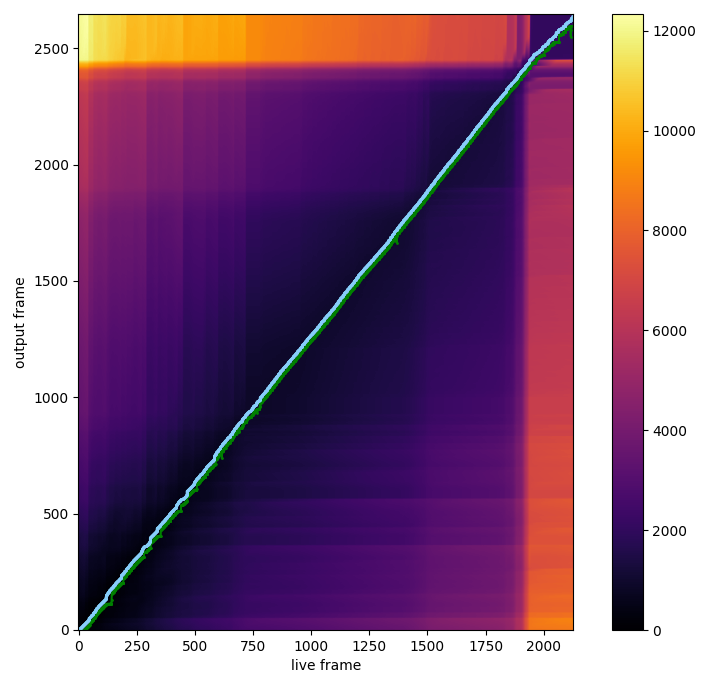
\includegraphics[scale=0.36]{ch4/fig-fast-offline-and-online-output.png}}
    \caption{快(135-175bpm)}
    \label{fig:fig-ch4-fast-tracking-results}
\end{figure}

\cref{fig:fig-ch4-accelerate-tracking-results}涵蓋了整個慢到快的速度區間,
可以看到\cref{fig:accelerate-tracking-output}在前面速度較慢時輸出相同的點的狀況較多,
當現場音訊演奏越來越快,輸出點所連成的線的斜率越來越高。
在\cref{fig:accelerate-comparision-output}的表現上,與離線對齊路徑也是呈現一致。

\begin{figure}[H]
    %\captionsetup[subfigure]{labelformat=empty} % 完全隱藏圖號
    \centering
    \subcaptionbox
    {
    \label{fig:accelerate-tracking-output}}
    {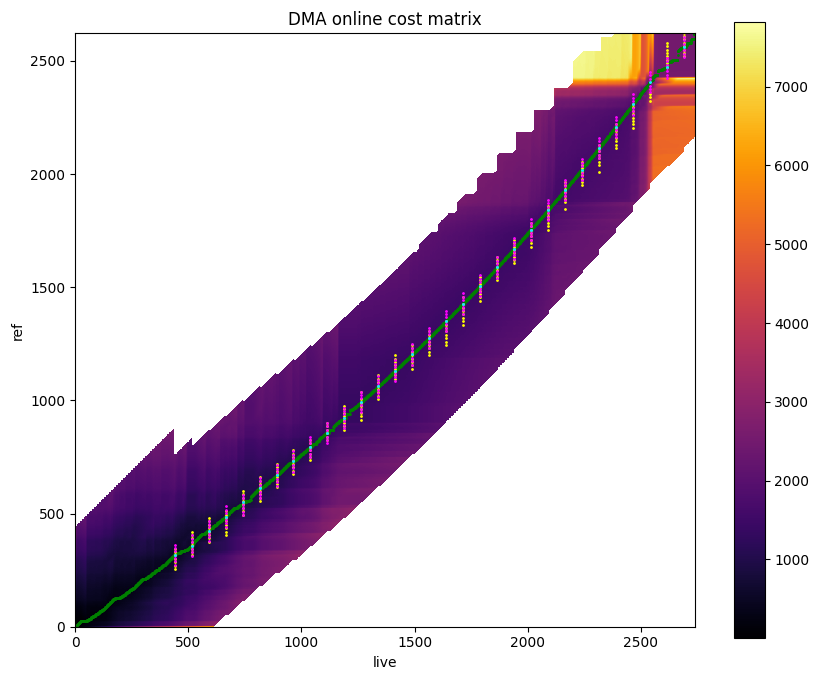
\includegraphics[scale=0.36]{ch4/fig-accelerate-tracking-system-output.png}}
    ~
    \subcaptionbox
    {
    \label{fig:accelerate-comparision-output}}
    {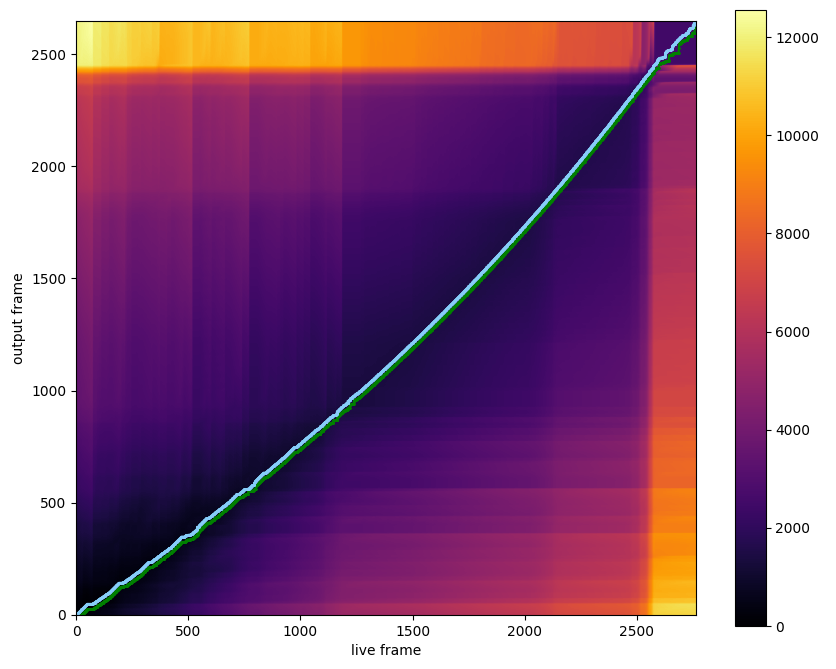
\includegraphics[scale=0.36]{ch4/fig-accelerate-offline-and-online-output.png}}
    \caption{加速(80$ \rightarrow $160bpm)}
    \label{fig:fig-ch4-accelerate-tracking-results}
\end{figure}

上述使用的MIDI檔案與結果音檔可從此連結~\cite{YuJieLin2024MidiTrackingResults}查看聆聽。

% cost matrix對齊圖
% 放MIDI隨機生成速度的那些評估圖

\subsection{系統在使用音源分離音訊做為參考特徵的追蹤結果}
為了評估系統是否在不同特徵下也能有好的追蹤結果,
我們使用與\ref{ch4-subst-midi-tracking-results}節相同的曲子,
在網路上找到由kopikostar演奏的小提琴與鋼琴合奏版本\cite{kopikostar2024Beethoven},
並對此混合音訊做音源分離,將分離結果作為參考音訊與伴奏音訊。
分離結果的音檔可至此連結聆聽~\cite{YuJieLin2024MusicSourceSeparation}。

我們實際演奏現場音訊,並演奏了四種不同速度,分別為110bpm、120bpm、130bpm與140bpm,
此四種速度為這首曲子最常出現的演奏速度。
演奏時,為了保持演奏速度的平穩,我們皆使用節拍器來輔助,
我們也演奏了自由速度版本,也就是不使用節拍器,與鋼琴互相配合演奏。
在演奏時使用AKG C519 M 電容式麥克風收錄音訊,監聽耳機為Sony MDR 7506,
並使用Focusrite Scarlett 2i2錄音介面處理類比與數位訊號。

由於沒有正確的伴奏音訊(Ground truth),因此我們無法使用\ref{ch4-subst-midi-tracking-results}節的方法來評估
與正確伴奏音訊的延遲。
因此我們改由計算系統輸出路徑與DTW離線對齊路徑的平均延遲幀數來評估系統在線上追蹤的表現是否與離線追蹤相當,
這邊的平均延遲幀數代表的是對於線上追蹤表現,是否提前或落後離線追蹤表現。

下圖為五種不同速度的對齊路徑結果圖,橫軸為現場音訊的時間點,縱軸為參考音訊的時間點,
(a)圖為追蹤系統在執行時所輸出的結果圖,
(b)圖為離線對齊路徑與線上對齊路徑的比較圖與平均延遲幀數。

\cref{fig:fig-ch4-mss-110bpm-tracking-results}為速度110bpm下的追蹤結果,
由\cref{fig:mss-110bpm-tracking-output}的xy軸可以看出現場音訊的速度比參考音訊要來的慢,
因此會出現等待的情況,例如live frame=700的時候。
\cref{fig:mss-110bpm-comparision-output}顯示了追蹤結果與離線計算結果的延遲為26.62幀,
約為532ms左右。

\begin{figure}[H]
    %\captionsetup[subfigure]{labelformat=empty} % 完全隱藏圖號
    \centering
    \subcaptionbox
    {
    \label{fig:mss-110bpm-tracking-output}}
    {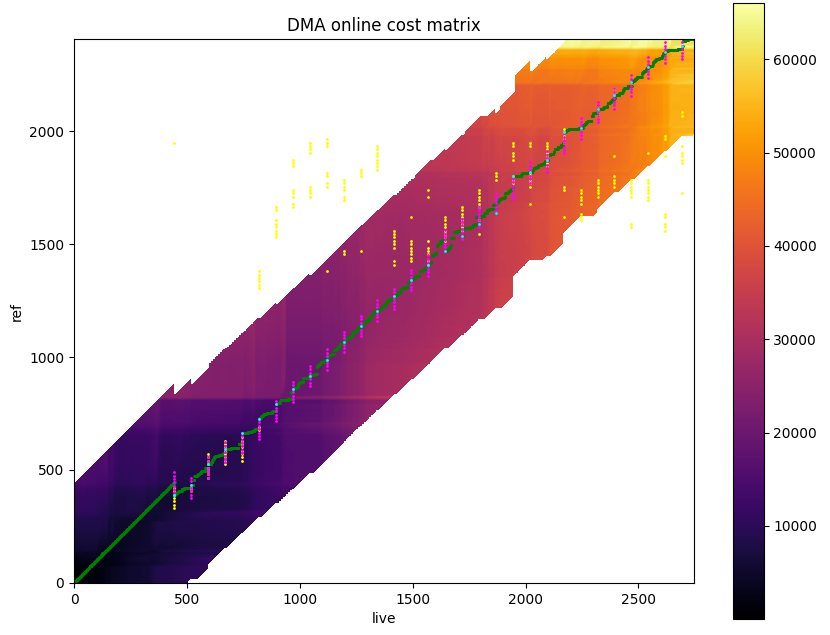
\includegraphics[scale=0.36]{ch4/fig-mss-110bpm-tracking-system-output.png}}
    ~
    \subcaptionbox
    {
    \label{fig:mss-110bpm-comparision-output}}
    {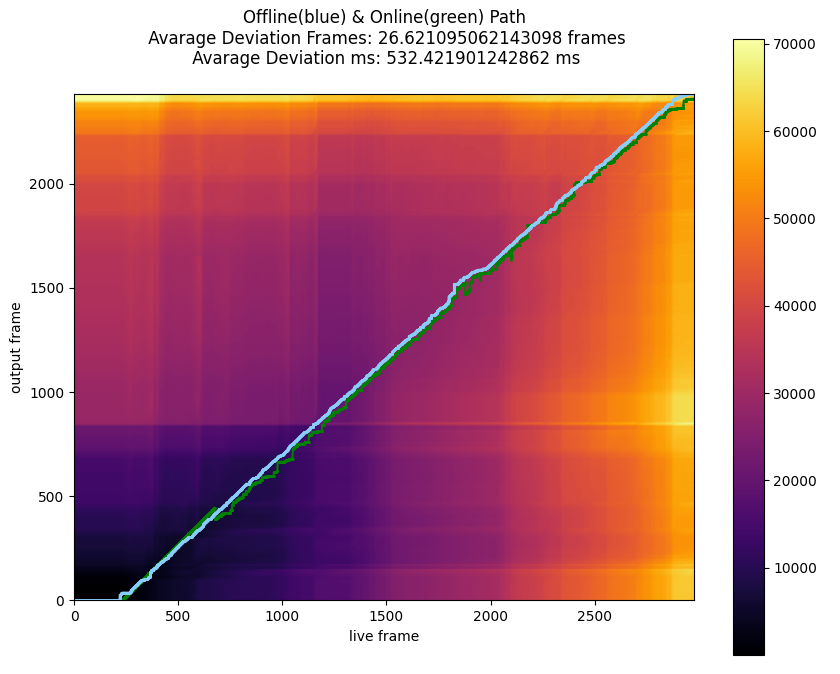
\includegraphics[scale=0.36]{ch4/fig-mss-110bpm-offline-and-online-output.png}}
    \caption{110bpm 平均延遲:26.62 幀}
    \label{fig:fig-ch4-mss-110bpm-tracking-results}
\end{figure}

\cref{fig:fig-ch4-mss-120bpm-tracking-results}為速度120bpm下的追蹤結果,
由\cref{fig:mss-120bpm-tracking-output}的xy軸可以看出現場音訊的速度也是比參考音訊的速度稍慢,
\cref{fig:mss-120bpm-comparision-output}顯示了追蹤結果與離線計算結果的延遲為27.98幀,
約為560ms左右。

\begin{figure}[H]
    %\captionsetup[subfigure]{labelformat=empty} % 完全隱藏圖號
    \centering
    \subcaptionbox
    {
    \label{fig:mss-120bpm-tracking-output}}
    {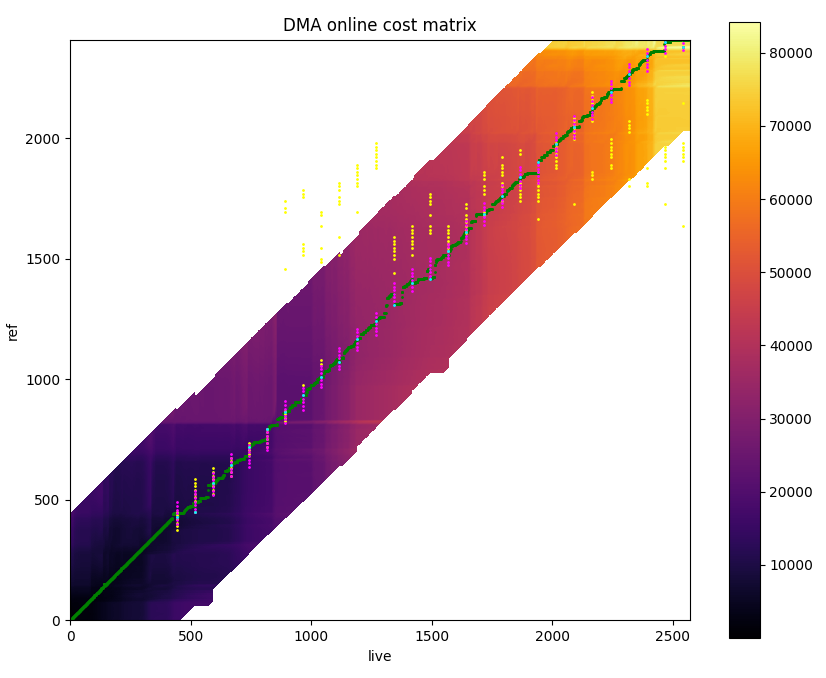
\includegraphics[scale=0.36]{ch4/fig-mss-120bpm-tracking-system-output.png}}
    ~
    \subcaptionbox
    {
    \label{fig:mss-120bpm-comparision-output}}
    {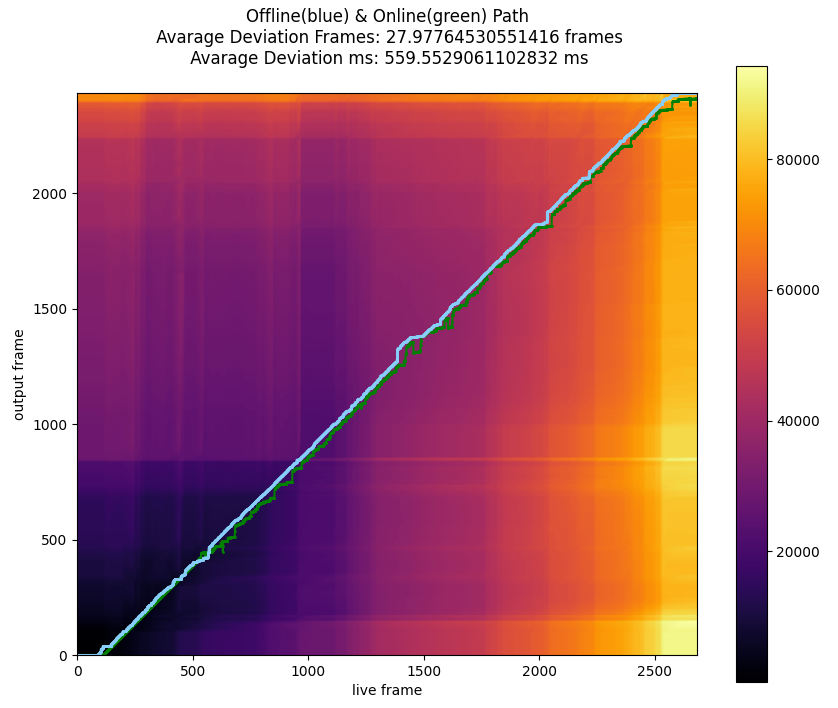
\includegraphics[scale=0.36]{ch4/fig-mss-120bpm-offline-and-online-output.png}}
    \caption{120bpm 平均延遲:27.98 幀}
    \label{fig:fig-ch4-mss-120bpm-tracking-results}
\end{figure}

\cref{fig:fig-ch4-mss-130bpm-tracking-results}為速度130bpm下的追蹤結果,
由\cref{fig:mss-130bpm-tracking-output}的xy軸可以看出現場音訊與參考音訊的速度較為相近,
但可能因為特徵差距的關係使追蹤結果並沒有比起前面的結果要好。
\cref{fig:mss-130bpm-comparision-output}顯示了追蹤結果與離線計算結果的延遲為37.49幀,
約為750ms左右。

\begin{figure}[H]
    %\captionsetup[subfigure]{labelformat=empty} % 完全隱藏圖號
    \centering
    \subcaptionbox
    {
    \label{fig:mss-130bpm-tracking-output}}
    {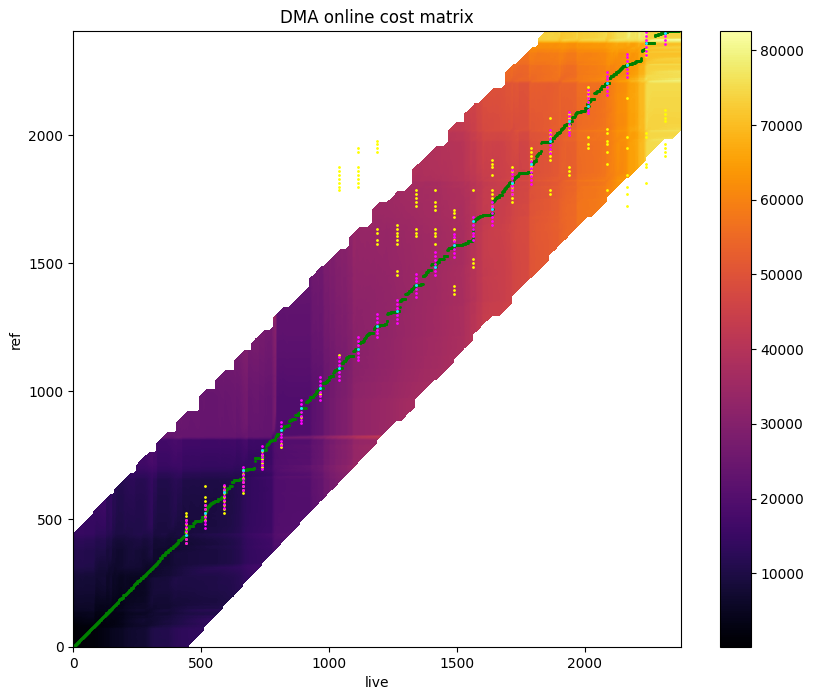
\includegraphics[scale=0.36]{ch4/fig-mss-130bpm-tracking-system-output.png}}
    ~
    \subcaptionbox
    {
    \label{fig:mss-130bpm-comparision-output}}
    {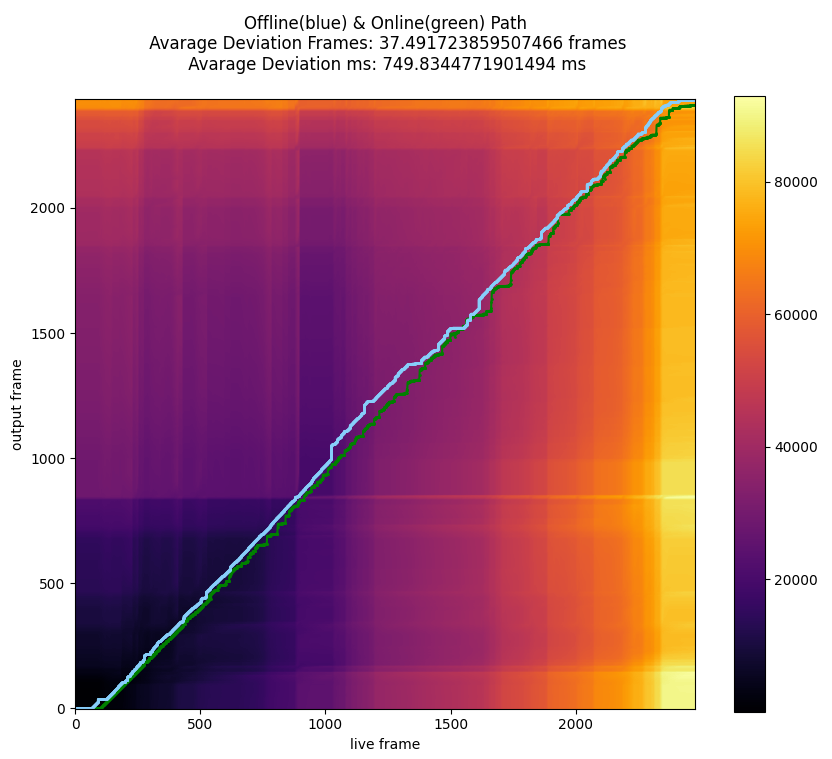
\includegraphics[scale=0.36]{ch4/fig-mss-130bpm-offline-and-online-output.png}}
    \caption{130bpm 平均延遲:37.49 幀}
    \label{fig:fig-ch4-mss-130bpm-tracking-results}
\end{figure}

\cref{fig:fig-ch4-mss-140bpm-tracking-results}為速度140bpm下的追蹤結果,
由\cref{fig:mss-140bpm-tracking-output}的xy軸可以看出現場音訊比參考音訊的速度稍快一些,
在live frame約500的時候,可以看到追蹤的路徑並不穩定,此時靠著RPE的粗略估計位置將ODTW對齊錯誤的地方拉回正軌。
\cref{fig:mss-140bpm-comparision-output}顯示了追蹤結果與離線計算結果的延遲為40.68幀,
約為814ms左右。

\begin{figure}[H]
    %\captionsetup[subfigure]{labelformat=empty} % 完全隱藏圖號
    \centering
    \subcaptionbox
    {
    \label{fig:mss-140bpm-tracking-output}}
    {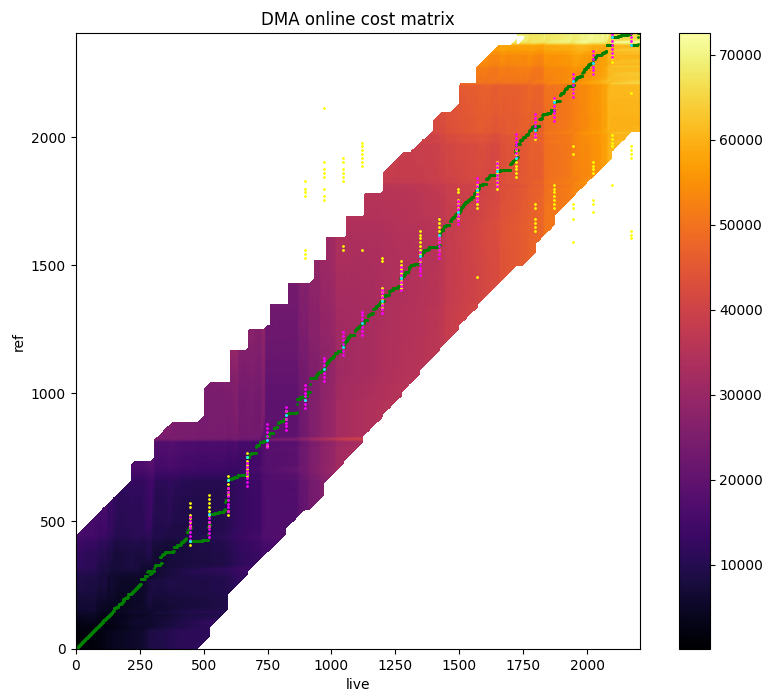
\includegraphics[scale=0.36]{ch4/fig-mss-140bpm-tracking-system-output.png}}
    ~
    \subcaptionbox
    {
    \label{fig:mss-140bpm-comparision-output}}
    {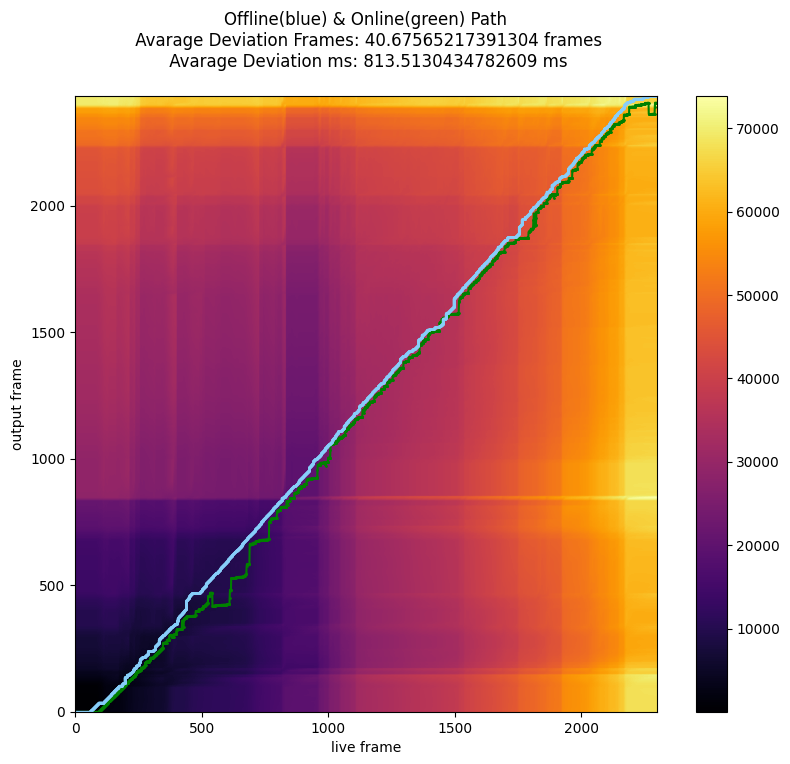
\includegraphics[scale=0.36]{ch4/fig-mss-140bpm-offline-and-online-output.png}}
    \caption{140bpm 平均延遲:40.68 幀}
    \label{fig:fig-ch4-mss-140bpm-tracking-results}
\end{figure}

\cref{fig:fig-ch4-mss-free-tracking-results}為自由速度下的追蹤結果,
由\cref{fig:mss-free-tracking-output}的xy軸可以看出現場音訊比參考音訊的速度稍慢一些,
在live frame約1500之後,可以看到追蹤的路徑並不穩定,我認為可能是這段的旋律是重複的,
因此可能在粗略估計的位置上無法精準的計算目前粗估位置,但最後還是有走回正軌。
\cref{fig:mss-free-comparision-output}顯示了追蹤結果與離線計算結果的延遲為28.43幀,
約為569ms左右。

\begin{figure}[H]
    %\captionsetup[subfigure]{labelformat=empty} % 完全隱藏圖號
    \centering
    \subcaptionbox
    {
    \label{fig:mss-free-tracking-output}}
    {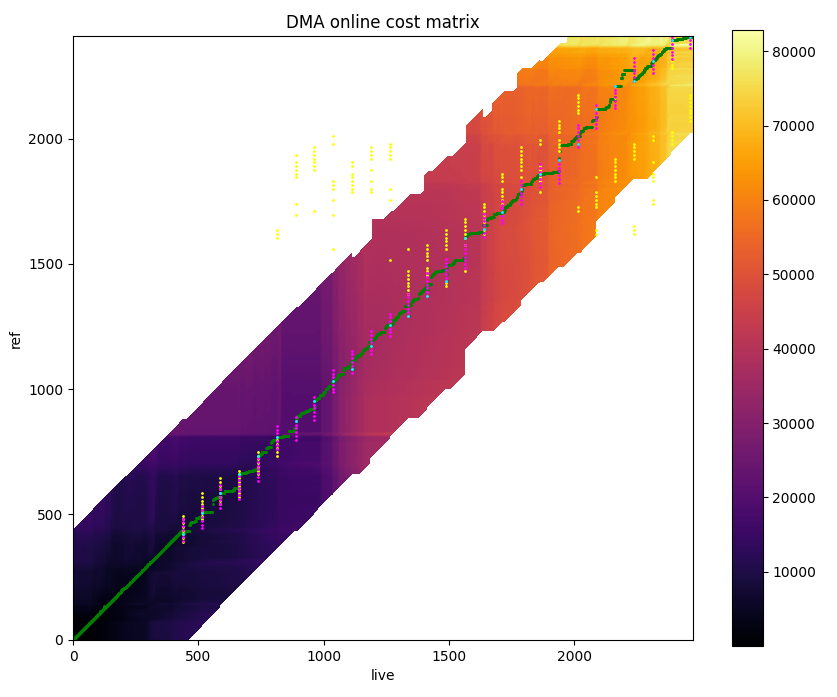
\includegraphics[scale=0.36]{ch4/fig-mss-free-tracking-system-output.png}}
    ~
    \subcaptionbox
    {
    \label{fig:mss-free-comparision-output}}
    {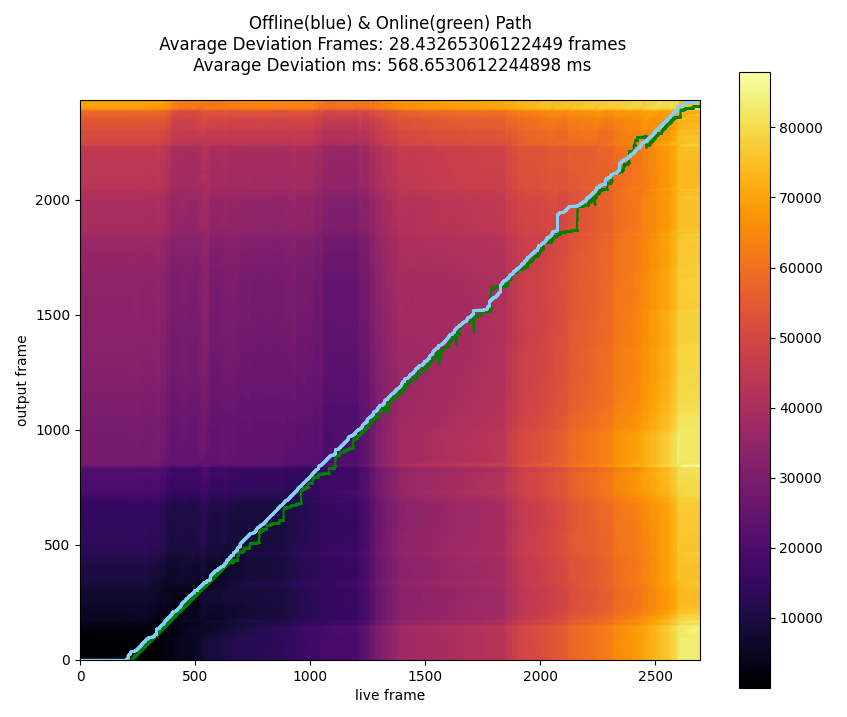
\includegraphics[scale=0.36]{ch4/fig-mss-free-offline-and-online-output.png}}
    \caption{自由速度 平均延遲:28.43 幀}
    \label{fig:fig-ch4-mss-free-tracking-results}
\end{figure}

由於參考音訊與現場音訊的特徵不一致,導致ODTW在計算對齊點時穩定性較為不足,
RPE估計出的位置也因為兩個音訊的特徵不夠相近,使粗略估計的位置偏差較嚴重,
因此追蹤結果圖大多數看起來比\ref{ch4-subst-midi-tracking-results}節的結果要差。
但可以看到在比較離線對齊路徑與線上對齊路徑的結果圖,大致上的路徑都與離線對齊路徑重合,
因此我們可以知道這兩個音訊在線上的最佳對齊路徑已經非常接近離線對齊路徑,
達到了即使使用不同特徵追蹤也能維持離線最佳對齊的效果。
另外可以看到比較圖中從第0幀到兩段路徑開始對齊的時間點是一致的,
代表我們的音樂偵測元件在判斷演奏者的演奏時間是精準的。
此外,我認為平均延遲都高達500ms以上可能是因為DTW在計算對齊路徑時,i與j都有遵守連續性的限制,
因此不會出現一次跳2格以上的路徑,且i是可以重複的;
但我們在計算ODTW時,在j方向是有可能出現一次跳2格以上的路徑,然而i為嚴格遞增,
因此造成兩個路徑在計算時,因為固定了i的位置,在$(t_j-t_i)$的差距可能會更大,
但實際聽起來並沒有延遲500ms那麼多。

我們也測試了使用同一人演奏的參考特徵來追蹤現場演奏的效果,
首先我們先錄製了與伴奏音訊完整對齊的音訊作為混合音訊,並將此混合音訊透過音源分離模型分離成參考音訊與伴奏音訊,
並使用這些音訊進行音樂追蹤。
接著現場演奏我們一樣採自由速度,
聆聽伴奏音訊來演奏,結果如\cref{fig:fig-ch4-free-ours-ref-tracking-results}所示,
可以看到線上對齊路徑與離線對齊路徑重合,代表系統輸出的路徑是最佳對齊位置,
在平均延遲上也比\cref{fig:fig-ch4-mss-free-tracking-results}要來的好。

\begin{figure}[H]
    %\captionsetup[subfigure]{labelformat=empty} % 完全隱藏圖號
    \centering
    \subcaptionbox
    {
    \label{fig:free-ours-ref-tracking-output}}
    {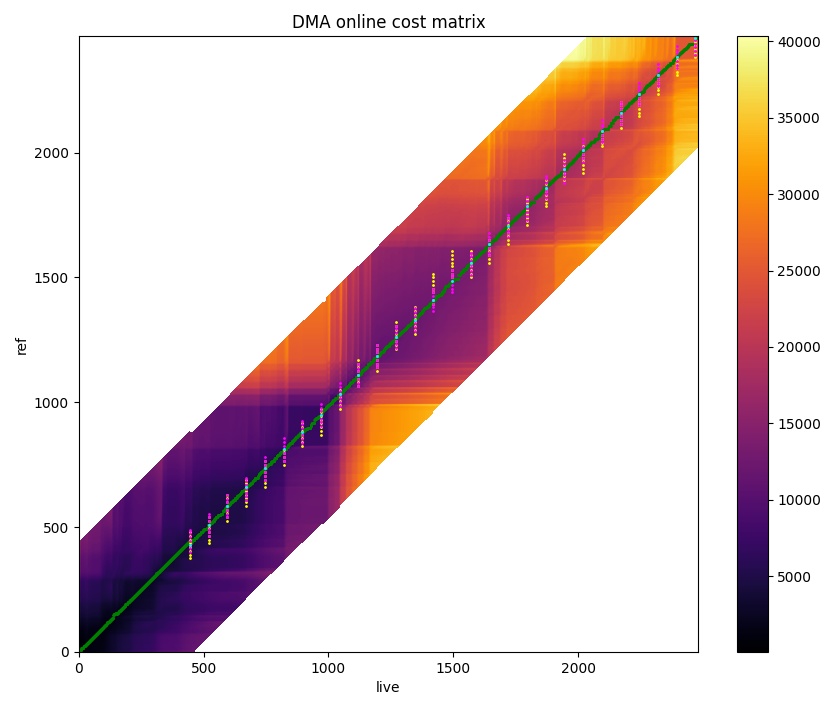
\includegraphics[scale=0.36]{ch4/fig-free-ours-ref-tracking-system-output.png}}
    ~
    \subcaptionbox
    {
    \label{fig:free-ours-ref-comparision-output}}
    {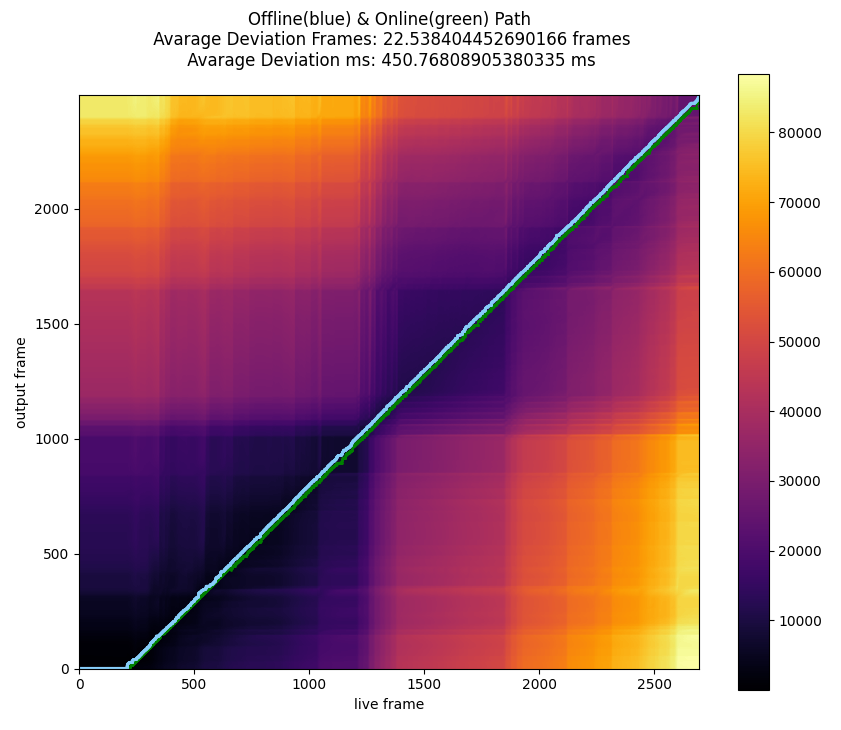
\includegraphics[scale=0.36]{ch4/fig-free-ours-ref-offline-and-online-output.png}}
    \caption{自由速度(參考音訊為同一人所演奏) 平均延遲:22.54 幀}
    \label{fig:fig-ch4-free-ours-ref-tracking-results}
\end{figure}
上述的結果音檔可從此連結~\cite{YuJieLin2024DiffFeatureTrackingResults}查看聆聽。

最後,根據~\cite{lin2021AIMusician}的紀錄,
~\cite{Lin2020AHumanComputerDuetSystem}的系統在偵測到觸發伴奏的平均延遲控制在0.1秒左右,
而本研究實際測試後,我們的系統可將偵測到觸發伴奏的平均延遲控制在0.05秒左右。

% \subsection{不同系統參數設定下的追蹤結果}
% 需測試


\pagebreak

\end{document}          % 實驗設計與結果
        \documentclass[class=NCU_thesis, crop=false]{standalone}
\begin{document}

\chapter{總結}

\section{未來展望}

\end{document}      % 結論
    %     \documentclass[class=NCU_thesis, crop=false]{standalone}
\usepackage{showexpl}

\begin{document}

\chapter{章名(章節示例)}
章內容內容內容內容內容 \\
內容內容內容

\section{節名}
節內容內容內容內容內容 \\
內容內容內容

\subsection{小節名}
內容內容內容 \\
內容內容內容

\subsubsection{小小節}
內容內容內容 \\
內容內容內容

\paragraph{段}
內容內容內容 \\
內容內容內容

\subparagraph{小段}
內容內容內容 \\
內容內容內容


\chapter{文字}
第一行。
仍是第一行。 \\
第二行。


\chapter{圖片}
\section{插入單一圖片}
\fig[0.15][fig:label_test][!hbt]{logo-Linux.png}[caption][short caption]

\section{插入多張圖片}
\begin{figure}[!hbt]
    %\captionsetup[subfigure]{labelformat=empty} % 完全隱藏圖號
    \centering
    \subcaptionbox
        {caption\_1
        \label{fig:subfig_fig1}}
        {\includegraphics[width=0.3\linewidth]{fig1.png}}
    ~
    \subcaptionbox
        {caption\_2
        \label{fig:subfig_fig2}}
        {\includegraphics[width=0.3\linewidth]{fig2.eps}}
    \vspace{\baselineskip} % 分隔上下列
    \subcaptionbox
        {caption\_3
        \label{fig:subfig_fig3}}
        {\includegraphics[width=0.6\linewidth]{fig3.png}}
    \caption{caption, 使用 \subref{fig:subfig_fig2}取得子圖(Debian)編號 }
    \label{fig:label}
\end{figure}


\chapter{表格}
\section{一般表格}
\begin{table}[h]
    \centering
    \caption{Solution}
    \begin{tabular}{| l | l |}
        \hline
        Component & Concentration(mM) \\ \hline
        \ce{NaCl} & 118.0 \\ \hline
    \end{tabular}
\end{table}

\section{自動折行表格}
\begin{table}[h]
    \centering
    \begin{tabularx}{\textwidth}{| l | X |}
        \hline
        short & short short \\ \hline
        long & long long long long long long long long long long  long long long long long long long long long long\\ \hline
    \end{tabularx}
\end{table}

\end{document}
    \backmatter          % book class 預設\backmatter 在\appendix 後面。因此.cls修改過\appendix 定義
        % This file has 3 types bibliography management, 
% \bibManType in config.tex choose it.
% 0. Embedded: write \bibitem in {thebibliography} environment.
% 1. BibTeX: Change bib files in \bibliography{}
% 2. biber / BibLaTeX: Add bibliography by \addbibresource{bibfile.bib} in macros_preamble.tex

\documentclass[class=NCU_thesis, crop=false]{standalone}

\begin{document}

\ifcase \bibManType 
    % 0 == Embedded %%%%%%%%%%%%%%%%%%%%%%%%%%%%%%%%%%%%%%%
    {\bibFontStyle\setstretch{\bibLineStretch}
    \begin{thebibliography}{99}

    \bibitem{cite_key_1}
        bibliography item detail.

    \bibitem{_sppmg/tw_thesis_template_????}
        TW\_Thesis\_Template,
        sppmg,
        \url{https://github.com/sppmg/TW_Thesis_Template},
        Embedded bibliography demo.

    \end{thebibliography}
    }
    
\or
    % 1 == BibTeX %%%%%%%%%%%%%%%%%%%%%%%%%%%%%%%%%%%%%%%%%
    \bibliographystyle{\bibStyle}
    {\bibFontStyle\setstretch{\bibLineStretch}
        \bibliography{demo} % {sample_1,sample_2,...,sample_n}
        % Note the lack of whitespace between the commas and the next bib file.
    }
    % % 1 == BibTeX %%%%%%%%%%%%%%%%%%%%%%%%%%%%%%%%%%%%%%%%%
    % \bibliographystyle{\IEEEtran}
    % {\bibFontStyle\setstretch{\bibLineStretch}
    %     \bibliography{demo, IEEEabrv} % {sample_1,sample_2,...,sample_n}
    %     % Note the lack of whitespace between the commas and the next bib file.
    % }
\or

    % 2 == biber / BibLaTeX %%%%%%%%%%%%%%%%%%%%%%%%%%%%%%%
    \printbibliography[title = {參考文獻}, heading = bibnumbered]
\fi



\end{document}
    % \appendix
    %     \documentclass[class=NCU_thesis, crop=false]{standalone}
\begin{document}

\chapter{裝置列表}

\begin{table}[!h]
    \centering
    \begin{tabularx}{\textwidth}{|l|l|X|}
        \hline
        裝置	     & 型號      & 說明 \\ \hline
        Linux    & Debian 9 & 世界好用的作業系統 \\ \hline
        Windows  & 10       & 防止人腦老化的工具 \\ \hline
    \end{tabularx}
    \caption{裝置列表}
    \label{table:list_device}
\end{table}

\end{document}
    %     \documentclass[class=NCU_thesis, crop=false]{standalone}
\begin{document}

\definecolor{Gray3}{gray}{0.8}

\chapter{Solutions}

\section{The solution}
\begin{table}[!h]
    \centering
    \begin{tabular}{| l | l |}
        \hline
        Component & Concentration(mM) \\ \hline
        \rowcolor{Gray3}
        \ce{NaCl} & 1.0 \\ \hline
        \ce{CaCl_2} & 2.0 \\ \hline
        \rowcolor{Gray3}
        \ce{NaCl} & 1.0 \\ \hline
        \ce{CaCl_2} & 2.0 \\ \hline
    \end{tabular}
    \caption{The solution}
\end{table}
\end{document}
    %     \documentclass[class=NCU_thesis, crop=false]{standalone}
\begin{document}
% Here demo instert whole code file. You can only insert code directly, 
% please read my tutorial or document of listings package.
% code style set in macros_preamble already.
% Supported language please read document of listings package or
% https://www.sharelatex.com/learn/Code_listing#!#Supported_languages

\chapter{程式碼}
\section{C}
\lstinputlisting[language=C]{hello_world_c.c}

\section{Matlab}
\lstinputlisting[language=matlab]{hello_world_matlab.m}

\section{IDL}
\lstinputlisting[language=IDL]{hello_world_idl.pro}
\end{document}

    %     \documentclass[class=NCU_thesis, crop=false]{standalone}

\begin{document}
\chapter{自動填單}
這裡試著幫各位自動填入部份資訊,其餘打勾、日期請手寫。有字體大小不符、位置歪掉等問題的話,請修改 appendix\_letter\_NCU.tex後直接編譯生成文件。

appendix\_letter\_NCU.tex中,每個句子(文字項目)都是獨立的大小與位置。 大小可由\textbackslash{}fs,調整。
\footnote{\textbackslash{}fs 使用 \textbackslash{}fontsize 做無級調整,並固定單行高度。 }
位置可由\textbackslash{}placetextbox 調整。語法如下:
\begin{lstlisting}[style=LatexStyle,caption={}]
\placetextbox{x(mm)}{y(mm)}
\end{lstlisting}
單位使用mm ,(0,0)位於左下角。建議調整時將``colorgrid''加入documentclass選項。(加入子檔的即可)
\begin{lstlisting}[style=LatexStyle,caption={}]
\documentclass[class=NCU_thesis, crop=false, colorgrid]{standalone}
\end{lstlisting}
colorgrid 將顯示格線(一小格是\SI{5}{\milli\metre})。

\begin{center}
{ \noindent\color{red}\bfseries\Large NCU English letters in the NCU\_en}
\end{center}

%%%%%%%%%%%%%%%%%%%%%%%%%%%%%%%%

% define \mprof 
\ExplSyntaxOn
    % Copy prof. list from config.tex
    \clist_gclear_new:N \g_sppmg_profs_cl
    \clist_gset:NV \g_sppmg_profs_cl \profs
    \clist_gpop:NNTF \g_sppmg_profs_cl \l_tmpa_tl {}{ \tl_clear:N \l_tmpa_tl}
    \cs_gset_eq:NN \mprof \l_tmpa_tl
\ExplSyntaxOff

\cleardoublepage
\pagestyle{empty}
\sffamily
% ------------------------------

% % 碩博士論文電子檔授權書
\IfFileExists{\letterAuthEl}{
\cleardoublepage\thispagestyle{empty}
\includepdf[pagecommand={   \placetextbox{100}{120}{\fs{17}\title}%
                            \placetextbox{95}{109}{\fs{17}\mprof}%
                            \placetextbox{69}{98}{\fs{17}\deptshort} }]%
{\letterAuthEl}}{}

% 碩博士紙本論文延後公開/下架申請書。(如需延後公開者,才需要裝訂於論文內頁)
\IfFileExists{\letterPubReq}{
\cleardoublepage\thispagestyle{empty}
\includepdf[pagecommand={   \placetextbox{128}{270}{\fs{17}\author}%
                            \placetextbox{70}{258}{\fs{17}\deptshort}%
                            \placetextbox{100}{233}{\fs{17}\title}%
                            \placetextbox{90}{219.3}{\fs{17}\mprof} }]%
{\letterPubReq}}{}

% 指導教授推薦書
\IfFileExists{\letterRecom}{
\cleardoublepage\thispagestyle{empty}
\includepdf[pagecommand={   \placetextbox{50}{159}{\fs{22}\deptshort}%
                            \placetextbox{118}{159}{\fs{22}\author}%
                            \placetextbox{105}{144}{\fs{22}\title}}%
]{\letterRecom}}{}

% 口試委員審定書
\IfFileExists{\letterVerif}{
\cleardoublepage\thispagestyle{empty}
\includepdf[pagecommand={   \placetextbox{63}{200.5}{\fs{22}\deptshort}%
                            \placetextbox{145}{200.5}{\fs{22}\author}%
                            \placetextbox{100}{170}{\fs{22}\title}}%
]{\letterVerif}}{}

% ------------------------------
\pagestyle{fancy}
\end{document}
\end{document}